\documentclass{beamer}
%\documentclass[handout]{beamer}


%%%%%%%%%%%%%
%% THEMES w/o navigaton
%\usetheme{default}
%\usetheme{Madrid}
%\usetheme{Pittsburgh}
%\usetheme{Boadilla}

%%%%%%%%%%%%%
%% THEMES w/ tree navigation
%\usetheme{Antibes}

%%%%%%%%%%%%%
%% THEMES w/ TOC sidebar
%\usetheme{Berkeley}
%\usetheme{PaloAlto}


%%%%%%%%%%%%%
%% THEMES w/ miniframe navigation
%\usetheme{Berlin}
%\usetheme{Darmstadt}
%\usetheme{Ilmenau}
%\usetheme{Singapore}
%\usetheme{Frankfurt}

%%%%%%%%%%%%%
%% THEMES w/ section/subsection titles
%\usetheme{Copenhagen}
%\usetheme{Warsaw}


%%%%%%%%%%%%%%%%%
%% CUSTOMIZED THEME %%%%
\usetheme{Marburg}

\makeatletter
  \setbeamertemplate{sidebar \beamer@sidebarside}
  {
    \beamer@tempdim=\beamer@sidebarwidth%
    \advance\beamer@tempdim by -6pt%
    \vskip4em%
    \insertverticalnavigation{\beamer@sidebarwidth}%
    \vfill
    \ifx\beamer@sidebarside\beamer@lefttext%
    \else%
      \usebeamercolor{normal text}%
      \llap{\usebeamertemplate***{navigation symbols}\hskip0.1cm}%
      \vskip2pt%
    \fi%
  }%

  \ifx\beamer@sidebarside\beamer@lefttext%
    \defbeamertemplate*{sidebar right}{sidebar theme}
    {%
      \vfill%
      \llap{\usebeamertemplate***{navigation symbols}\hskip0.1cm}%
      \vskip2pt}
  \fi

\setbeamertemplate{section in sidebar}%{sidebar theme}
{%
  \vbox{%
    \vskip1ex%
    \beamer@sidebarformat{3pt}{section in sidebar}{\insertsectionheadnumber
~\insertsectionhead}%
  }%
}
\setbeamertemplate{section in sidebar shaded}%{sidebar theme}
{%
  \vbox{%
    \vskip1ex%
    \beamer@sidebarformat{3pt}{section in sidebar shaded}{\insertsectionheadnumber
~\insertsectionhead}%
  }%
}
\makeatother



%% COLOR THEMES %%
%\usecolortheme{dove}
%\usecolortheme{beaver}


%%%%%%%%%%%%%%%

\usepackage{multirow}

\usepackage{tikz}
\usetikzlibrary{arrows}

\DeclareMathOperator*{\argmax}{arg\,max}
\DeclareMathOperator*{\argmin}{arg\,min}
%\DeclareMathOperator*{\Em}{E_w(x=x^{(m)},h)}
\DeclareMathOperator*{\Em}{E_w(x^{(m)},h)}
\DeclareMathOperator*{\E}{E_w(x,h)}
\DeclareMathOperator*{\Es}{E(x,h)}
%\DeclareMathOperator*{\nw}{\nabla_{w_{ij}}}
\DeclareMathOperator*{\nw}{\partial_{w_{ij}}}
\newcommand{\btheta}{\boldsymbol \theta }
\newcommand{\bi}{\begin{itemize}}
\newcommand{\ei}{\end{itemize}}
\newcommand{\be}{\begin{enumerate}}
\newcommand{\ee}{\end{enumerate}}


%\setbeamertemplate{footline}{\hfill\insertframenumber/\inserttotalframenumber}

\setbeamertemplate{footline}[text line]{%
  \parbox{\linewidth}{\hfill (p.\insertframenumber})}
\setbeamertemplate{navigation symbols}{}


\setbeamertemplate{bibliography item}{}


\makeatletter
\def\blfootnote{\xdef\@thefnmark{}\@footnotetext}
\makeatother

\makeatother


\title{Deep Learning Tutorial}
\author{Kevin Duh}
\institute{Nara Institute of Science \& Technology / Johns Hopkins HLTCOE}
\date{Oct 18, 2015}


\AtBeginSubsection[]
{
  \begin{frame}
    \small{\frametitle{Outline}
    \tableofcontents[currentsection,currentsubsection]
	}
  \end{frame}
}

\begin{document}

\begin{frame}
\titlepage
\end{frame}


%%%%%%%%%%%%%
\begin{frame}
\frametitle{What is Deep Learning?}
A family of methods that uses deep architectures to learn high-level feature representations
\centerline{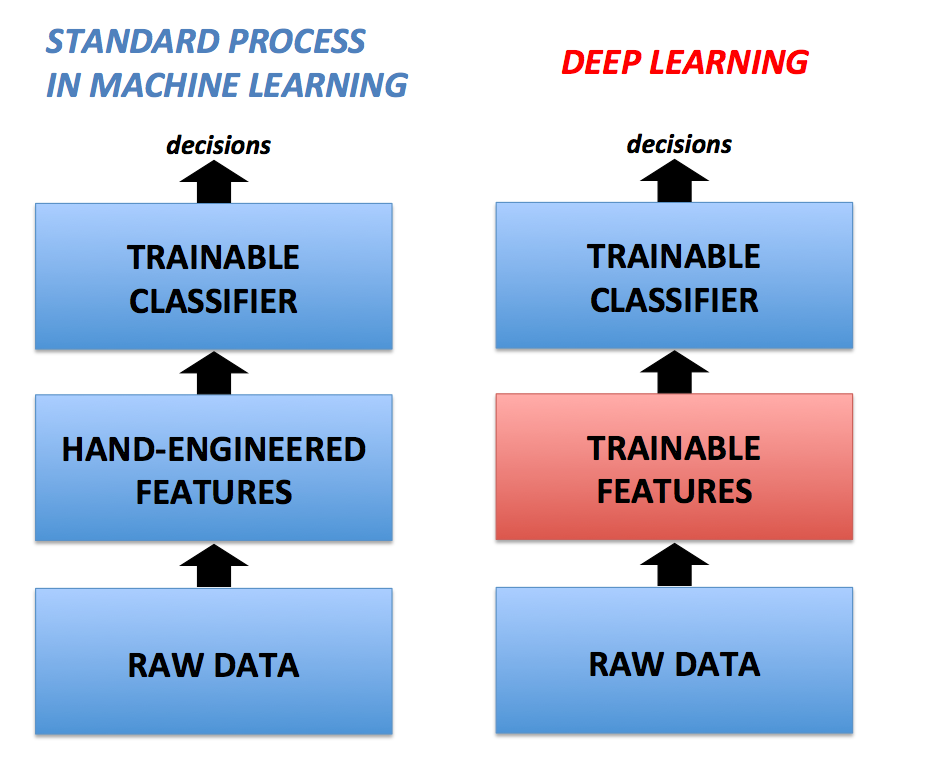
\includegraphics[scale=0.27]{figs/deep_vs_conventional_learning}}
\end{frame}

%%%%%%%%%%%%%
\begin{frame}
\frametitle{What got me excited in Deep Learning}
Automatically trained features make sense! \cite{lee09convolutional}\\[0.2cm]
Input: Images (raw pixels)\\
$\rightarrow$ Output: Features of Edges, Body Parts, Full Faces

\centerline{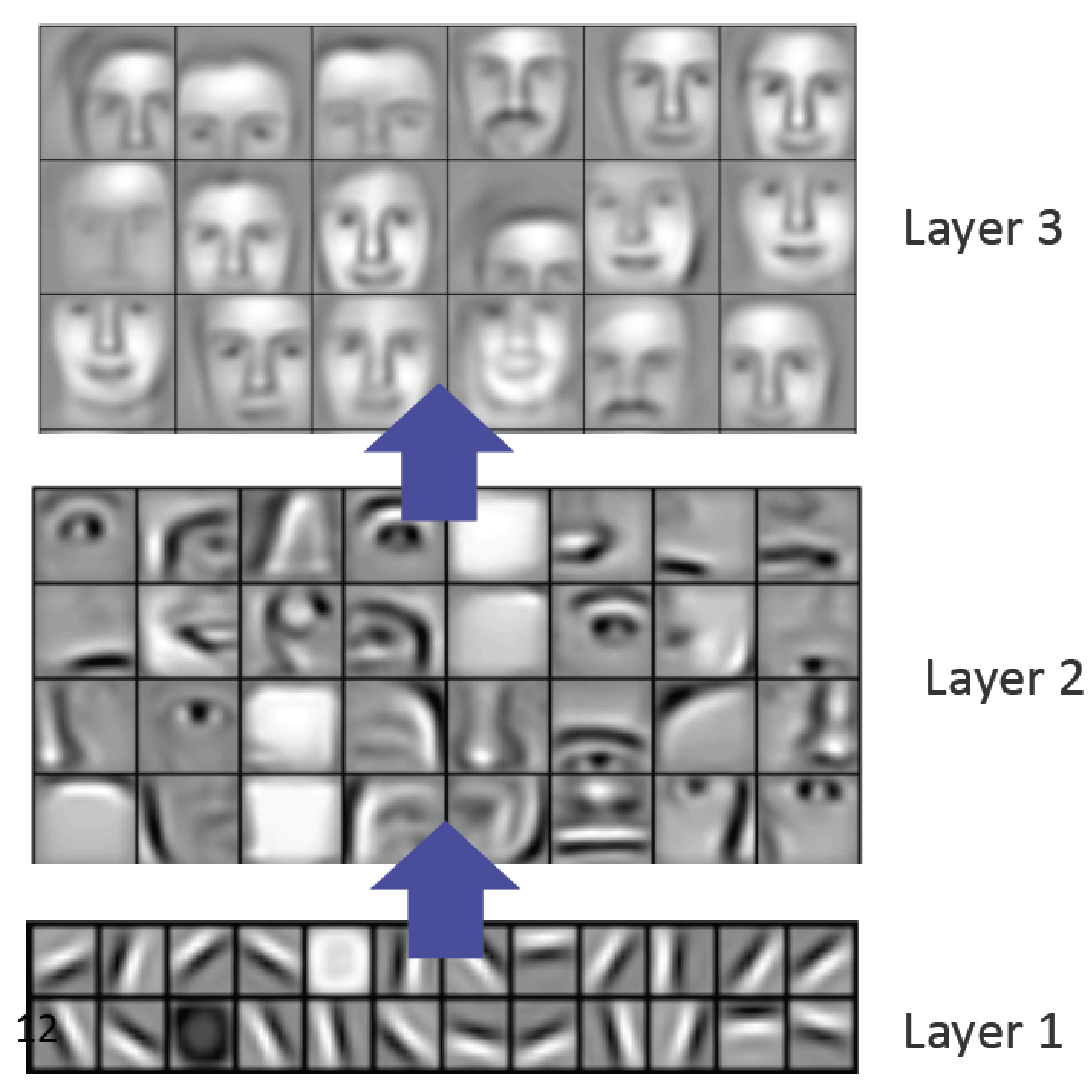
\includegraphics[scale=0.35]{figs/lee09example}}
\end{frame}


%%% 1. BASICS
%SECTION%%%%%%%%%%%%%%%%%%%
\section[Basics]{1. Deep Learning Basics}
\begin{frame}
\small{\frametitle{Outline}
\tableofcontents
}
\end{frame}
%%%%%%%%%%%%%%%%%%%%

%% 
\begin{frame}
\frametitle{This is a long talk, so...}
\bi
\item Please interrupt with questions/comments anytime.
\item Feel free to come and go as desired.
\ei
\end{frame}

%% SUBSECTION%%%%%
\subsection[Neural Network]{Neural Networks (1-layer, 2-layer)}

%%%%%%%%%%%%%
\begin{frame}
\frametitle{Problem Setup}
\bi
\item Training Data: a set of $(x^{(m)},y^{(m)})_{m=\{1,2,..M\}}$ pairs 
	\bi
	\item Input $x^{(m)} \in R^d$
	\item Output $y^{(m)}=\{0,1\}$ 
	\ei
\item Goal: Learn function $f: x \rightarrow y$ to predict correctly on new inputs $x$.
\pause
\bi
\item Step 1: Choose a function model family:
	\bi
	\item e.g. logistic regression, support vector machines, neural networks
	\ei
\pause
\item Step 2: Optimize parameters $w$ on the Training Data
	\bi 
	\item e.g. minimize loss function $\min_{w} \sum_{m=1}^M  ( f_w(x^{(m)}) - y^{(m)} )^2$
	\ei
\ei
\ei
\end{frame}

%%%%%%%%%%%%%
\begin{frame}
\frametitle{Logistic Regression (1-layer net)}
\bi
\item Function model: $f(x)=\sigma(w^T \cdot x)$
	\bi
	\item Parameters: vector $w \in R^d$
	\item $\sigma$ is a non-linearity, e.g. sigmoid: $\sigma(z) = 1/(1+\exp(-z))$
	\ei
\centerline{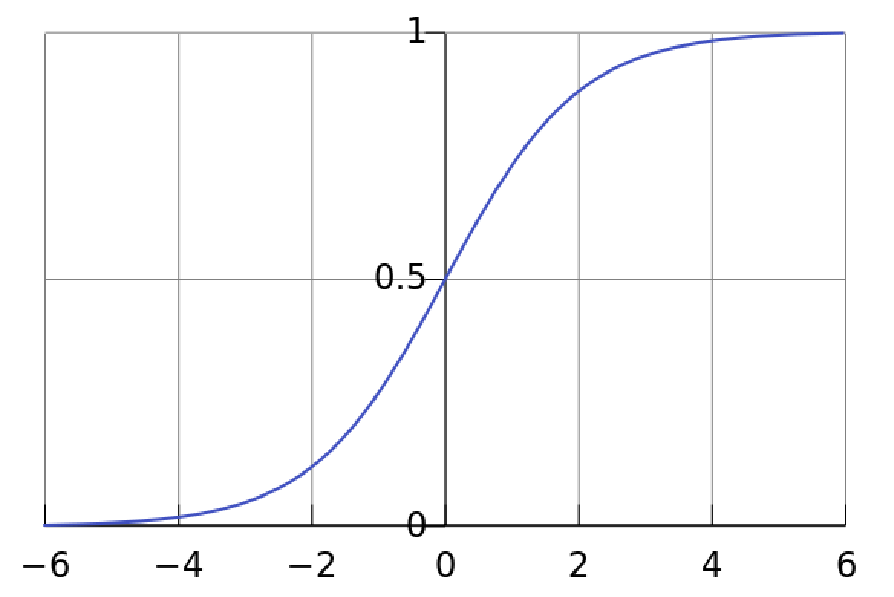
\includegraphics[scale=0.3]{figs/sigmoid}}
\pause
\item Non-linearity will be important in expressiveness multi-layer nets. Other non-linearities, e.g., $tanh(z)=(e^z-e^{-z}) / (e^z+e^{-z})$
\ei
\end{frame}


%%%%%%%%%%%%%
\begin{frame}
\frametitle{Gradient Descent for Logistic Regression }
\bi
\item Assume Squared-Error$^*$ $Loss(w) = \frac{1}{2} \sum_{m}  ( \sigma(w^T x^{(m)}) - y^{(m)} )^2$
\pause
%\item Gradient: $\nabla_w Loss = \sum_m {\color{red} ( \sigma(w^T x^{(m)}) - y^{(m)} )} {\color{blue} (\sigma(w^Tx^{(m)}) (1- \sigma(w^Tx^{(m)}) )} x^{(m)}$
\item Gradient: $\nabla_w Loss = \sum_m {\color{red} \left[ \sigma(w^T x^{(m)}) - y^{(m)} \right]} {\color{blue} \sigma'(w^Tx^{(m)})} x^{(m)}$
	\bi
	\pause
	\item Define input into non-linearity  ${\color{blue} in^{(m)} = w^Tx^{(m)}}$
	\item General form of gradient: $\sum_m{\color{red} Error^{(m)}} * {\color{blue} \sigma'(in^{(m)})} * x^{(m)}$
	\item Derivative of sigmoid $\sigma'(z) = \sigma(z) (1-\sigma(z))$
	\ei
\pause 
\item Gradient Descent Algorithm: 
	\be
	\item Initialize $w$ randomly
	\item Update until convergence: $w \leftarrow w - \gamma( \nabla_w Loss )$
	\ee
\item Stochastic gradient descent (SGD) algorithm:
	\be
	\item Initialize $w$ randomly
	\item Update until convergence: $w \leftarrow w - \gamma({\color{red} Error^{(m)}} * {\color{blue} \sigma'(in^{(m)})} * x^{(m)})$
	\ee
\ei
\vspace{-0.8cm}
\blfootnote{\hspace{-0.4cm}*An alternative is Cross-Entropy loss: $\sum_m~y^{(m)} \log(\sigma(w^Tx^{(m)}))+(1-y^{(m)}) \log(1-\sigma(w^Tx^{(m)}))$ }

\end{frame}

%%%%%%%%%%%%
\begin{frame}
\frametitle{Stochastic Gradient Descent (SGD)}
\bi
\item Gradient Descent Algorithm: 
	\be
	\item Initialize $w$ randomly
	\item Update until convergence: $w \leftarrow w - \gamma( \nabla_w Loss )$
	\ee
\item Stochastic gradient descent (SGD) algorithm:
	\be
	\item Initialize $w$ randomly
	\item Update until convergence: $w \leftarrow w - \gamma(\frac{1}{|B|}\sum_{m \in B}{\color{red} Error^{(m)}} * {\color{blue} \sigma'(in^{(m)})} * x^{(m)})$\\
          where minibatch $B$ ranges from e.g. 1-100 samples
	\ee
\pause
\item Learning rate $\gamma$:
  \bi
  \item For convergence, should decrease with each iteration $t$ through samples
  \item e.g. $\gamma_t = \frac{1}{\lambda * t} $ or $\gamma_t = \frac{\gamma_0}{1 + \gamma_0 * \lambda * t}$
  \ei
\ei

\end{frame}

%%%%%%%%%%%%%
\begin{frame}
\frametitle{SGD Pictorial View}
\bi
\item Loss objective contour plot: \begin{small}$\frac{1}{2} \sum_{m}  ( \sigma(w^T x^{(m)}) - y^{(m)} )^2 + ||w||$\end{small}
\bi
	\item Gradient descent goes in steepest descent direction
	\item SGD is noisy descent (but faster per iteration)
\ei
\ei
\centerline{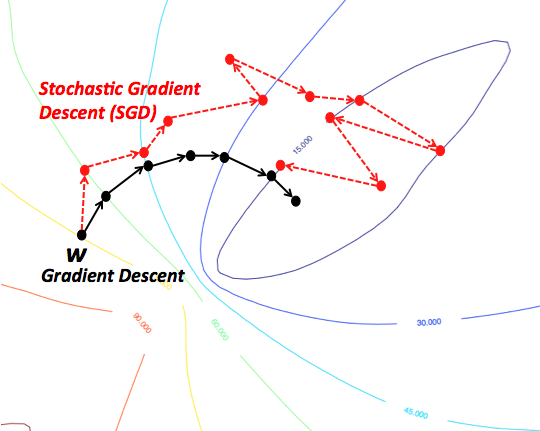
\includegraphics[scale=0.4]{figs/sgd_contour}}
\end{frame}


%%%%%%%%%%%%%
\begin{frame}
\frametitle{2-layer Neural Networks}
\begin{tikzpicture}[->,>=stealth',shorten >=1pt,auto,node distance=3cm,
  thick,main node/.style={circle,fill=blue!20,draw,font=\sffamily\Large\bfseries}]

  \node[main node] (1) at (1,0) {$x_1$};
  \node[main node] (2) at (3,0) {$x_2$};
  \node[main node] (3) at (5,0) {$x_3$};
  \node[main node] (4) at (7,0) {$x_4$};
  \node[main node] (h1) at (2,2) {$h_1$};
  \node[main node] (h2) at (4,2) {$h_2$};
  \node[main node] (h3) at (6,2) {$h_3$};
  \node[main node] (y) at (4,4) {$y$};

   \node(xi) at (0,0) {$x_i$};
   \node(wij) at (0,1) {${\color{red} w_{ij}}$};
   \node(hj) at (0,2) {$h_j$};
   \node(wj) at (0,3) {${\color{blue} w_{j}}$};

	

  \path[every node/.style={font=\sffamily\small}]
    (1) edge node [left] {${\color{red} w_{11}}$} (h1)
    (2) edge node {} (h1)
    (3) edge node {} (h1)
    (4) edge node {} (h1)
    (1) edge node [left] {${\color{red} w_{12}}$} (h2)
    (2) edge node {} (h2)
    (3) edge node {} (h2)
    (4) edge node {} (h2)
    (1) edge node {} (h3)
    (2) edge node {} (h3)
    (3) edge node {} (h3)
    (4) edge node {} (h3)
    (h1) edge node [left] {${\color{blue} w_1}$} (y)
    (h2) edge node [left] {${\color{blue} w_2}$} (y)
    (h3) edge node [left] {${\color{blue} w_3}$} (y)
    ;
\end{tikzpicture}

\vspace{4mm}
\begin{math}
f(x)=\sigma(\sum_j w_j \cdot h_j)
= \sigma(\sum_j {\color{blue} w_j} \cdot \sigma(\sum_i {\color{red} w_{ij}}  x_i))
\end{math}\\
\pause
\vspace{0.3cm}
Hidden units $h_j$'s can be viewed as new "features" from combining $x_i$'s
\blfootnote{\hspace{-0.5cm}Called Multilayer Perceptron (MLP), but more like multilayer logistic regression}
\end{frame}


%%%%%%%%%%%%%%%%
\begin{frame}
\frametitle{Expressive Power of Non-linearity}
\bi
\item A deeper architecture is more expressive than a shallow one given same number of nodes
\cite{bishop95book}
\bi
	\item 1-layer nets only model linear hyperplanes
	\item 2-layer nets can model any continuous function (given sufficient nodes)
	\item $>$3-layer nets can do so with fewer nodes
\ei
\ei
\centerline{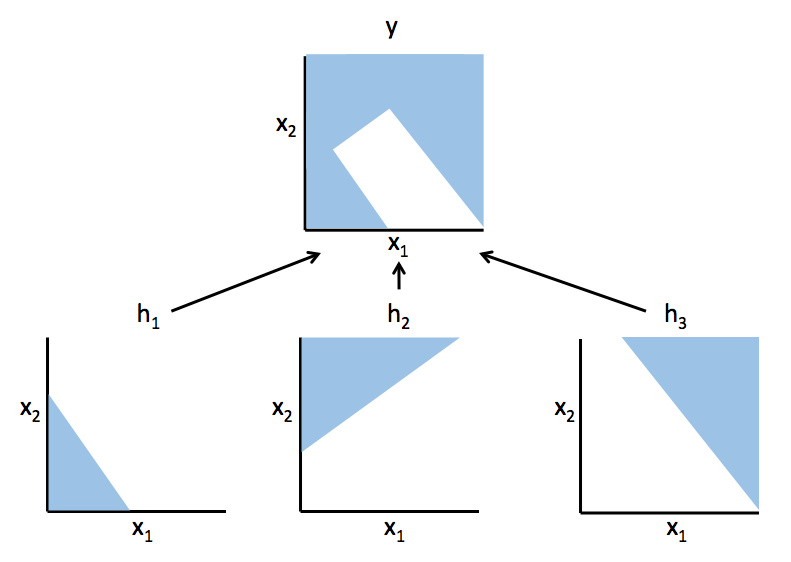
\includegraphics[scale=0.27]{figs/twolayer_nonlinearity}}
\end{frame}



%%%%%%%%%%%%%
\begin{frame}
\frametitle{Training Neural Nets: Back-propagation}
\begin{tikzpicture}[->,>=stealth',shorten >=1pt,auto,node distance=3cm,
  thick,main node/.style={circle,fill=blue!20,draw,font=\sffamily\Large\bfseries}]

  \node[main node] (1) at (1,0) {$x_1$};
  \node[main node] (2) at (3,0) {$x_2$};
  \node[main node] (3) at (5,0) {$x_3$};
  \node[main node] (4) at (7,0) {$x_4$};
  \node[main node] (h1) at (2,2) {$h_1$};
  \node[main node] (h2) at (4,2) {$h_2$};
  \node[main node] (h3) at (6,2) {$h_3$};
  \node[main node] (y) at (4,4) {$y$};

   \node(xi) at (0,0) {$x_i$};
   \node(wij) at (0,1) {$w_{ij}$};
   \node(hj) at (0,2) {$h_j$};
   \node(wj) at (0,3) {$w_{j}$};

	
  \draw[blue,ultra thick,-latex,->] (6.8,0.5) -- node[below right]{Predict $f(x^{(m)})$} (6.8,4);
  \draw[red,ultra thick,-latex,<-] (9.8,0.5) -- node[above left]{Adjust weights} (9.8,4);


  \path[every node/.style={font=\sffamily\small}]
    (1) edge node [left] {$w_{11}$} (h1)
    (2) edge node {} (h1)
    (3) edge node {} (h1)
    (4) edge node {} (h1)
    (1) edge node [left] {$w_{12}$} (h2)
    (2) edge node {} (h2)
    (3) edge node {} (h2)
    (4) edge node {} (h2)
    (1) edge node {} (h3)
    (2) edge node {} (h3)
    (3) edge node {} (h3)
    (4) edge node {} (h3)
    (h1) edge node [left] {$w_1$} (y)
    (h2) edge node [left] {$w_2$} (y)
    (h3) edge node [left] {$w_3$} (y)
    ;
\end{tikzpicture}

1. For each sample, compute $f(x^{(m)}) = \sigma(\sum_j w_j \cdot \sigma(\sum_i w_{ij}  x_i^{(m)}))$\\
2. If $f(x^{(m)})\ne y^{(m)}$, back-propagate error and adjust weights $\{w_{ij}, w_j\}$. 
\end{frame}

%%%%%%%%%%%%%
\begin{frame}
\frametitle{Derivatives of the weights}
Assume two outputs $(y_1, y_2)$ per input $x$,\\ and loss per sample:
$Loss = \sum_k \frac{1}{2} \left[ \sigma(in_k)   - y_k \right]^2 $

\begin{center}
\scalebox{0.7}{
\begin{tikzpicture}[->,>=stealth',shorten >=1pt,auto,node distance=3cm,
  thick,main node/.style={circle,fill=blue!20,draw,font=\sffamily\Large\bfseries}]

  \node[main node] (1) at (1,0) {$x_1$};
  \node[main node] (2) at (3,0) {$x_2$};
  \node[main node] (3) at (5,0) {$x_3$};
  \node[main node] (4) at (7,0) {$x_4$};
  \node[main node] (h1) at (2,2) {$h_1$};
  \node[main node] (h2) at (4,2) {$h_2$};
  \node[main node] (h3) at (6,2) {$h_3$};
  \node[main node] (y1) at (3,4) {$y_1$};
  \node[main node] (y2) at (5,4) {$y_2$};

 \node(xi) at (0,0) {$x_i$};
   \node(wij) at (0,1) {$w_{ij}$};
   \node(hj) at (0,2) {$h_j$};
   \node(wjk) at (0,3) {$w_{jk}$};
   \node(yk) at (0,4) {$y_{k}$};


  \path[every node/.style={font=\sffamily\small}]
    (1) edge node {} (h1)
    (2) edge node {} (h1)
    (3) edge node {} (h1)
    (4) edge node {} (h1)
    (1) edge node {} (h2)
    (2) edge node {} (h2)
    (3) edge node {} (h2)
    (4) edge node {} (h2)
    (1) edge node {} (h3)
    (2) edge node {} (h3)
    (3) edge node {} (h3)
    (4) edge node {} (h3)
    (h1) edge node {} (y1)
    (h2) edge node {}  (y1)
    (h3) edge node {} (y1)
    (h1) edge node {} (y2)
    (h2) edge node {}  (y2)
    (h3) edge node {} (y2)
    ;
\end{tikzpicture}
}
\end{center}

\pause
$ \frac{\partial Loss}{ \partial w_{jk}}
= {\color{red} \frac{\partial Loss}{ \partial in_k}} {\color{blue} \frac{ \partial in_k}{ \partial w_{jk}}}
= {\color{red} \delta_k} {\color{blue} \frac{\partial (\sum_j w_{jk} h_j)}{\partial w_{jk}} }
= {\color{red} \delta_k} {\color{blue} h_j}$

\pause
$ \frac{\partial Loss}{ \partial w_{ij}}
= {\color{red} \frac{\partial Loss}{ \partial in_j}} {\color{blue} \frac{ \partial in_j}{ \partial w_{ij}}}
= {\color{red} \delta_j} {\color{blue} \frac{\partial (\sum_j w_{ij} x_i)}{\partial w_{ij}} }
= {\color{red} \delta_j} {\color{blue} x_i}$

\pause
${\color{red} \delta_k = \frac{\partial}{\partial in_k} \left( \sum_k \frac{1}{2}  \left[ \sigma(in_k)   - y_k \right]^2\right)
= \left[ \sigma(in_k)-y_k \right] \sigma'(in_k) }$

\pause
${\color{red} \delta_j =  \sum_k  \frac{\partial Loss}{\partial in_k} \frac{\partial in_k}{\partial in_j} = \sum_k \delta_k
\cdot \frac{\partial}{\partial in_j}\left( \sum_j w_{jk} \sigma(in_j) \right) = \left[\sum_k \delta_k w_{jk}\right] \sigma'(in_j)}$


\end{frame}


%%%%%%%%%%%%%
\begin{frame}
\frametitle{Training Neural Nets: Back-propagation�}
All updates involve some {\color{red} scaled error from output} $*$ {\color{blue} input feature}:\\
\bi
\item $ \frac{\partial Loss}{ \partial w_{jk}} = {\color{red} \delta_k} {\color{blue} h_j}$
where ${\color{red} \delta_k = \left[ \sigma(in_k)-y_k \right] \sigma'(in_k) }$
\item $ \frac{\partial Loss}{ \partial w_{ij}} = {\color{red} \delta_j} {\color{blue} x_i}$
where ${\color{red} \delta_j = \left[\sum_k \delta_k w_{jk}\right] \sigma'(in_j)}$
\ei
First compute {\color{red} $\delta_k$} from final layer, then {\color{red} $\delta_j$} for previous layer and iterate.

\scalebox{1}{
\begin{tikzpicture}[->,>=stealth',shorten >=1pt,auto,node distance=3cm,
  thick,main node/.style={circle,fill=blue!20,draw,font=\sffamily\Large\bfseries}]

  \node[main node] (1) at (1,0) {$x_1$};
  \node[main node] (2) at (3,0) {$x_2$};
  \node[main node] (3) at (5,0) {$x_3$};
  \node[main node] (4) at (7,0) {$x_4$};
  \node[main node] (h1) at (2,2) {$h_1$};
  \node[main node] (h2) at (4,2) {$h_2$};
  \node[main node] (h3) at (6,2) {$h_3$};
  \node[main node] (y1) at (3,4) {$y_1$};
  \node[main node] (y2) at (5,4) {$y_2$};


   \node(xi) at (0,0) {$x_i$};
   \node(wij) at (0,1) {$w_{ij}$};
   \node(hj) at (0,2) {$h_j$};
   \node(wjk) at (0,3) {$w_{jk}$};
   \node(yk) at (0,4) {$y_{k}$};

   \node(deltah3) at (8.6,2.6) {${\color{red} \delta_{j=h_3} = [\delta_{k=y_1}w_{31} + \delta_{k=y_2}w_{32}]\sigma'(in_{h_3}) }$};
   \node(deltay1) at (4,4) {${\color{red} \delta_{k=y_1}}$};
   \node(deltay2) at (6,4) {${\color{red} \delta_{k=y_2}}$};

  \path[every node/.style={font=\sffamily\small}]
    (1) edge node {} (h1)
    (2) edge node {} (h1)
    (3) edge node {} (h1)
    (4) edge node {} (h1)
    (1) edge node {} (h2)
    (2) edge node {} (h2)
    (3) edge node {} (h2)
    (4) edge node {} (h2)
    (1) edge node {} (h3)
    (2) edge node {} (h3) 
    (3) edge node {} (h3)
    (4) edge node [right] {$ \frac{\partial Loss}{ \partial w_{ij}}$} (h3)
    (h1) edge node {} (y1)
    (h2) edge node {}  (y1)
    (h3) edge node [right] {${\color{red} w_{31}}$} (y1)
    (h1) edge node {} (y2)
    (h2) edge node {}  (y2)
    (h3) edge node [right] {${\color{red} w_{32}}$} (y2)
    ;
\end{tikzpicture}
}

\end{frame}

%% SUBSECTION%%%%%
\subsection[Computation Graph]{Computation Graphs and Deep Learning Toolkits}

%%%%%%%%%%%%%%%%
\begin{frame}
\frametitle{Current models are becoming more complex}
\vspace{0.5cm}
Do you want to take the derivative of this? \\
\vspace{0.5cm}
\centerline{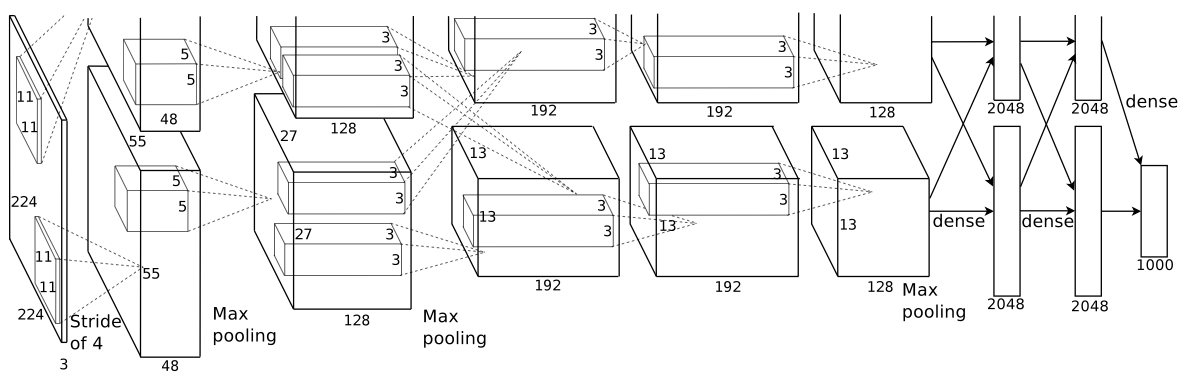
\includegraphics[scale=0.25]{figs/alexnet}}
\bi
\item AlexNet for image classification \cite{krizhevsky12imagenet}
\ei
\end{frame}

%%%%%%%%%%%%%%%%
\begin{frame}
\frametitle{Computation Graphs}
\bi
\item All computations can be viewed on a graph: 
\item e.g. 2-layer MLP: 
\begin{math}
y = softmax(W^{(2)} \cdot \sigma(W^{(1)}\cdot X+B^{(1)}) + B^{(2)}) 
\end{math}\\
\ei
\centerline{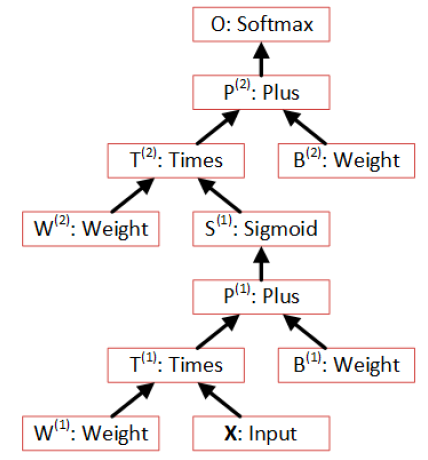
\includegraphics[scale=0.3]{figs/cntk1}}
\blfootnote{Figure from MSR CNTK tech report \cite{yu14cntk}\\\hspace{1cm} *$softmax(a_k)=\exp(a_k)/\sum_j\exp(a_j)$}
\end{frame}

%%%%%%%%%%%%%%%%
\begin{frame}
\frametitle{Computation Graphs}
\bi
\item All computations can be viewed on a graph: 
\item e.g. 2-layer MLP with {\color{red} shared weights}: 
\begin{math}
y = softmax(W^{(1)} \cdot \sigma(W^{(1)}\cdot X+B^{(1)}) + B^{(2)}) 
\end{math}\\
\ei
\centerline{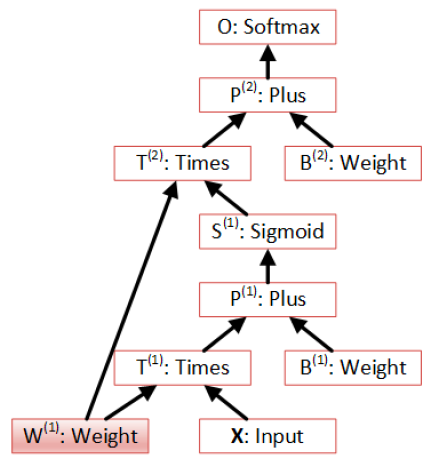
\includegraphics[scale=0.3]{figs/cntk2}}
\blfootnote{Figure from MSR CNTK tech report \cite{yu14cntk}\\\hspace{1cm} *$softmax(a_k)=\exp(a_k)/\sum_j\exp(a_j)$}
\end{frame}

%%%%%%%%%%%%%%%%
\begin{frame}
\frametitle{Computation Graphs}
\bi
\item All computations can be viewed on a graph: 
\item e.g. Computing the {\color{red} loss term} of the MLP
\ei
\centerline{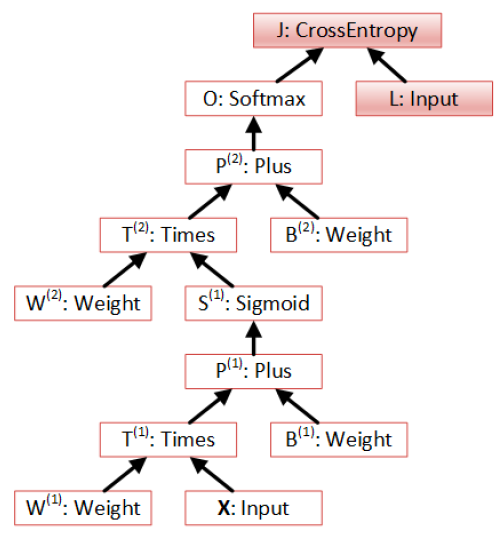
\includegraphics[scale=0.3]{figs/cntk3}}
\blfootnote{Figure from MSR CNTK tech report \cite{yu14cntk}\\\hspace{1cm} *$softmax(a_k)=\exp(a_k)/\sum_j\exp(a_j)$}
\end{frame}


%%%%%%%%%%%%%%%%
\begin{frame}
\frametitle{Toolkits enable rapid experimentation of various architectures}
Popular toolkits: Theano, Torch, pylearn2, Caffe, CNTK, CNN, Kaldi, etc.
\be
\item Compiles mathematical expression to graph
\item Implements basic operation for each node
\item Handles scheduling and batching of foward/backward computation
\item Also, GPU or fast math library support
\ee
\end{frame}


%% SUBSECTION%%%%%
\subsection[Why Deep is Hard]{Why Deep Architectures are Hard}

%%%%%%%%%%%%%%%%
\begin{frame}
\frametitle{Potential of Deep Architecture}
\begin{columns}
\begin{column}{0.5\textwidth}
\centerline{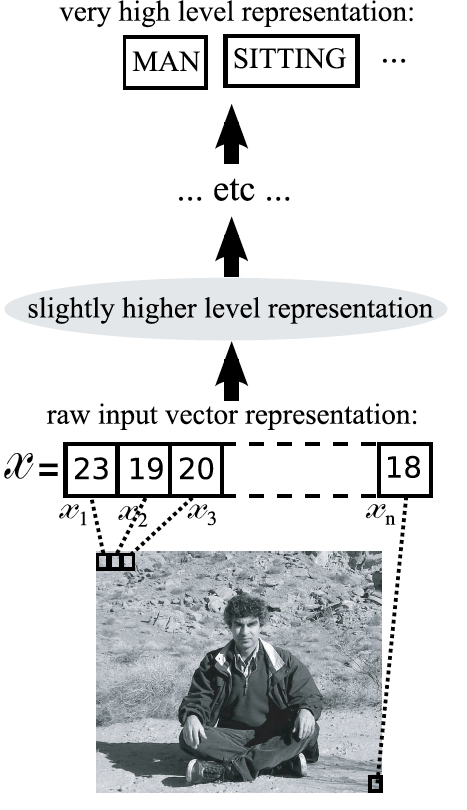
\includegraphics[scale=0.27]{figs/bengio_sitting}}
\textit{*Figure from \cite{bengio09book}}
\end{column}
\begin{column}{0.5\textwidth}
\begin{center}
\begin{tikzpicture}[-,>=stealth',shorten >=1pt,auto,node distance=3cm,
  thick,main node/.style={circle,fill=blue!20,draw,font=\sffamily\Large\bfseries}]

  \node[main node] (x1) at (0,0) {$x_1$};
  \node[main node] (x2) at (2,0) {$x_2$};
  \node[main node] (x3) at (4,0) {$x_3$};
  \node[main node] (h1) at (0,2) {$h_1$};
  \node[main node] (h2) at (2,2) {$h_2$};
  \node[main node] (h3) at (4,2) {$h_3$};
  \node[main node] (h'1) at (0,4) {$h'_1$};
  \node[main node] (h'2) at (2,4) {$h'_2$};
  \node[main node] (h'3) at (4,4) {$h'_3$};
  \node[main node] (y) at (2,6) {$y$};

  \path[every node/.style={font=\sffamily\small}]
    (x1) edge node {} (h1)
    (x1) edge node {} (h2)
    (x1) edge node {} (h3)
    (x2) edge node {} (h1)
    (x2) edge node {} (h2)
    (x2) edge node {} (h3)
    (x3) edge node {} (h1)
    (x3) edge node {} (h2)
    (x3) edge node {} (h3)
    (h1) edge node {} (h'1)
    (h1) edge node {} (h'2)
    (h1) edge node {} (h'3)
    (h2) edge node {} (h'1)
    (h2) edge node {} (h'2)
    (h2) edge node {} (h'3)
    (h3) edge node {} (h'1)
    (h3) edge node {} (h'2)
    (h3) edge node {} (h'3)
    (h'1) edge node {} (y)
    (h'2) edge node {} (y)
    (h'3) edge node {} (y) ;

\end{tikzpicture}
\end{center}
\end{column}
\end{columns}
\end{frame}


%%%%%%%%%%%%%%%%
\begin{frame}
\frametitle{Difficulties of Deep Architecture}
\begin{columns}
\begin{column}{0.5\textwidth}
\textbf{Vanishing gradient problem} in Backpropagation
\bi
\item $ \frac{\partial Loss}{ \partial w_{ij}} = {\color{red} \frac{\partial Loss}{ \partial in_j}} {\color{blue} \frac{ \partial in_j}{ \partial w_{ij}}}  = {\color{red} \delta_j}x_i$
\item ${\color{red} \delta_j =  \left[\sum_{j+1} \delta_{j+1} w_{j(j+1)}\right] \sigma'(in_j)}$
\item ${\color{red} \delta_j}$ may vanish after repeated multiplication
\item Also, exploding gradient problem!
\ei
\end{column}
\begin{column}{0.5\textwidth}
\begin{center}
\begin{tikzpicture}[-,>=stealth',shorten >=1pt,auto,node distance=3cm,
  thick,main node/.style={circle,fill=blue!20,draw,font=\sffamily\Large\bfseries}]

  \node[main node] (x1) at (0,0) {$x_1$};
  \node[main node] (x2) at (2,0) {$x_2$};
  \node[main node] (x3) at (4,0) {$x_3$};
  \node[main node] (h1) at (0,2) {$h_1$};
  \node[main node] (h2) at (2,2) {$h_2$};
  \node[main node] (h3) at (4,2) {$h_3$};
  \node[main node] (h'1) at (0,4) {$h'_1$};
  \node[main node] (h'2) at (2,4) {$h'_2$};
  \node[main node] (h'3) at (4,4) {$h'_3$};
  \node[main node] (y) at (2,6) {$y$};

   \node(wij) at (4.3,1) {${\color{red}w_{ij}}$};
   \node(wjj1) at (4.6,3) {${\color{red}w_{j(j+1)}}$};
   
  \path[every node/.style={font=\sffamily\small}]
    (x1) edge node {} (h1)
    (x1) edge node {} (h2)
    (x1) edge node {} (h3)
    (x2) edge node {} (h1)
    (x2) edge node {} (h2)
    (x2) edge node {} (h3)
    (x3) edge node {} (h1)
    (x3) edge node {} (h2)
    (x3) edge node {} (h3)
    (h1) edge node {} (h'1)
    (h1) edge node {} (h'2)
    (h1) edge node {} (h'3)
    (h2) edge node {} (h'1)
    (h2) edge node {} (h'2)
    (h2) edge node {} (h'3)
    (h3) edge node {} (h'1)
    (h3) edge node {} (h'2)
    (h3) edge node {} (h'3)
    (h'1) edge node {} (y)
    (h'2) edge node {} (y)
    (h'3) edge node {} (y) ;

\end{tikzpicture}
\end{center}
\end{column}
\end{columns}
\end{frame}



%%%%%%%%%%%%%%%%
\begin{frame}
\frametitle{Training Difficulties \cite{erhan09difficulty}}
\bi
\item MNIST digit classification task
\item Train neural net by Backpropagation (random initialization of $w_{ij}$) 
\ei 
\centerline{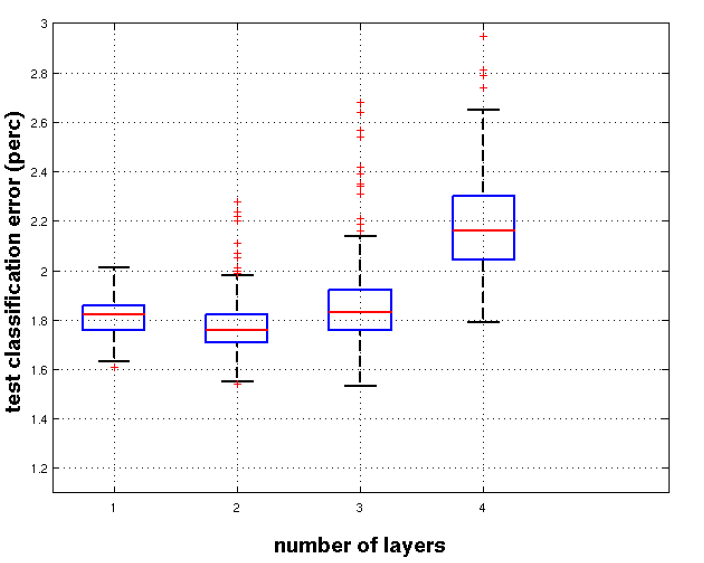
\includegraphics[scale=0.36]{figs/difficulty_backprop}}
\end{frame}



%% SUBSECTION%%%%%
\subsection[2006 Breakthrough]{The Breakthrough in 2006}

%%%%%%%%%%%%%%%%
\begin{frame}
\frametitle{Layer-wise Pre-training \cite{hinton06dbn}}
First, train one layer at a time, optimizing data-likelihood objective $P(x)$
\begin{center}
\begin{tikzpicture}[-,>=stealth',shorten >=1pt,auto,node distance=3cm,
  thick,main node/.style={circle,fill=blue!20,draw,font=\sffamily\Large\bfseries}]

  \node[main node] (x1) at (0,0) {$x_1$};
  \node[main node] (x2) at (2,0) {$x_2$};
  \node[main node] (x3) at (4,0) {$x_3$};
  \node[main node] (h1) at (0,2) {$h_1$};
  \node[main node] (h2) at (2,2) {$h_2$};
  \node[main node] (h3) at (4,2) {$h_3$};
  \node[main node] (h'1) at (0,4) {$h'_1$};
  \node[main node] (h'2) at (2,4) {$h'_2$};
  \node[main node] (h'3) at (4,4) {$h'_3$};
  \node[main node] (y) at (2,6) {$y$};

  \draw[blue,ultra thick,-latex,<->] (5,0) -- node[right]{Train Layer1} (5,2);


  \path[every node/.style={font=\sffamily\small}]
    (x1) edge node {} (h1)
    (x1) edge node {} (h2)
    (x1) edge node {} (h3)
    (x2) edge node {} (h1)
    (x2) edge node {} (h2)
    (x2) edge node {} (h3)
    (x3) edge node {} (h1)
    (x3) edge node {} (h2)
    (x3) edge node {} (h3)
    (h1) edge node {} (h'1)
    (h1) edge node {} (h'2)
    (h1) edge node {} (h'3)
    (h2) edge node {} (h'1)
    (h2) edge node {} (h'2)
    (h2) edge node {} (h'3)
    (h3) edge node {} (h'1)
    (h3) edge node {} (h'2)
    (h3) edge node {} (h'3)
    (h'1) edge node {} (y)
    (h'2) edge node {} (y)
    (h'3) edge node {} (y) ;

\end{tikzpicture}
\end{center}
\end{frame}



%%%%%%%%%%%%%%%%
\begin{frame}
\frametitle{Layer-wise Pre-training \cite{hinton06dbn}}
First, train one layer at a time, optimizing data-likelihood objective $P(x)$
\begin{center}
\begin{tikzpicture}[-,>=stealth',shorten >=1pt,auto,node distance=3cm,
  thick,main node/.style={circle,fill=blue!20,draw,font=\sffamily\Large\bfseries}]

  \node[main node] (x1) at (0,0) {$x_1$};
  \node[main node] (x2) at (2,0) {$x_2$};
  \node[main node] (x3) at (4,0) {$x_3$};
  \node[main node] (h1) at (0,2) {$h_1$};
  \node[main node] (h2) at (2,2) {$h_2$};
  \node[main node] (h3) at (4,2) {$h_3$};
  \node[main node] (h'1) at (0,4) {$h'_1$};
  \node[main node] (h'2) at (2,4) {$h'_2$};
  \node[main node] (h'3) at (4,4) {$h'_3$};
  \node[main node] (y) at (2,6) {$y$};

  \draw[blue,ultra thick,-latex,<->] (5,2) -- node[right]{Train Layer2} (5,4);
  \draw[blue,ultra thick,-latex,<->] (5,0) -- node[right]{Keep Layer1 fixed} (5,2);

  \path[every node/.style={font=\sffamily\small}]
    (x1) edge node {} (h1)
    (x1) edge node {} (h2)
    (x1) edge node {} (h3)
    (x2) edge node {} (h1)
    (x2) edge node {} (h2)
    (x2) edge node {} (h3)
    (x3) edge node {} (h1)
    (x3) edge node {} (h2)
    (x3) edge node {} (h3)
    (h1) edge node {} (h'1)
    (h1) edge node {} (h'2)
    (h1) edge node {} (h'3)
    (h2) edge node {} (h'1)
    (h2) edge node {} (h'2)
    (h2) edge node {} (h'3)
    (h3) edge node {} (h'1)
    (h3) edge node {} (h'2)
    (h3) edge node {} (h'3)
    (h'1) edge node {} (y)
    (h'2) edge node {} (y)
    (h'3) edge node {} (y) ;

\end{tikzpicture}
\end{center}
\end{frame}

%%%%%%%%%%%%%%%%
\begin{frame}
\frametitle{Layer-wise Pre-training \cite{hinton06dbn}}
Finally, fine-tune labeled objective $P(y|x)$ by Backpropagation
\begin{center}
\begin{tikzpicture}[-,>=stealth',shorten >=1pt,auto,node distance=3cm,
  thick,main node/.style={circle,fill=blue!20,draw,font=\sffamily\Large\bfseries}]

  \node[main node] (x1) at (0,0) {$x_1$};
  \node[main node] (x2) at (2,0) {$x_2$};
  \node[main node] (x3) at (4,0) {$x_3$};
  \node[main node] (h1) at (0,2) {$h_1$};
  \node[main node] (h2) at (2,2) {$h_2$};
  \node[main node] (h3) at (4,2) {$h_3$};
  \node[main node] (h'1) at (0,4) {$h'_1$};
  \node[main node] (h'2) at (2,4) {$h'_2$};
  \node[main node] (h'3) at (4,4) {$h'_3$};
  \node[main node] (y) at (2,6) {$y$};

  \draw[red,ultra thick,-latex,->] (5,0) -- node[below right]{Predict f(x)} (5,6);
  \draw[red,ultra thick,-latex,->] (8,6) -- node[above left]{Adjust weights} (8,0);

  \path[every node/.style={font=\sffamily\small}]
    (x1) edge node {} (h1)
    (x1) edge node {} (h2)
    (x1) edge node {} (h3)
    (x2) edge node {} (h1)
    (x2) edge node {} (h2)
    (x2) edge node {} (h3)
    (x3) edge node {} (h1)
    (x3) edge node {} (h2)
    (x3) edge node {} (h3)
    (h1) edge node {} (h'1)
    (h1) edge node {} (h'2)
    (h1) edge node {} (h'3)
    (h2) edge node {} (h'1)
    (h2) edge node {} (h'2)
    (h2) edge node {} (h'3)
    (h3) edge node {} (h'1)
    (h3) edge node {} (h'2)
    (h3) edge node {} (h'3)
    (h'1) edge node {} (y)
    (h'2) edge node {} (y)
    (h'3) edge node {} (y) ;

\end{tikzpicture}
\end{center}
\end{frame}

%%%%%%%%%%%%%%%%
\begin{frame}
\frametitle{Layer-wise Pre-training \cite{hinton06dbn}}
\textbf{Key Idea:\\
Focus on modeling the input $P(X)$ better with each successive layer.\\
Worry about optimizing the task $P(Y|X)$ later.}
\begin{quote}\color{blue}{"If you want to do computer vision, first learn computer graphics." -- Geoff Hinton} \end{quote}

\begin{columns}
\begin{column}{0.7\textwidth}
\begin{center}
\scalebox{0.7}{
\begin{tikzpicture}[-,>=stealth',shorten >=1pt,auto,node distance=3cm,
  thick,main node/.style={circle,fill=blue!20,draw,font=\sffamily\Large\bfseries}]

  \node[main node] (x1) at (0,0) {$x_1$};
  \node[main node] (x2) at (2,0) {$x_2$};
  \node[main node] (x3) at (4,0) {$x_3$};
  \node[main node] (h1) at (0,2) {$h_1$};
  \node[main node] (h2) at (2,2) {$h_2$};
  \node[main node] (h3) at (4,2) {$h_3$};
  \node[main node] (h'1) at (0,4) {$h'_1$};
  \node[main node] (h'2) at (2,4) {$h'_2$};
  \node[main node] (h'3) at (4,4) {$h'_3$};
  \node[main node] (y) at (2,6) {$y$};

  \draw[blue,ultra thick,-latex,<->] (5,2) -- node[right]{Train Layer2} (5,4);
  \draw[blue,ultra thick,-latex,<->] (5,0) -- node[right]{Train Layer1} (5,2);

  \path[every node/.style={font=\sffamily\small}]
    (x1) edge node {} (h1)
    (x1) edge node {} (h2)
    (x1) edge node {} (h3)
    (x2) edge node {} (h1)
    (x2) edge node {} (h2)
    (x2) edge node {} (h3)
    (x3) edge node {} (h1)
    (x3) edge node {} (h2)
    (x3) edge node {} (h3)
    (h1) edge node {} (h'1)
    (h1) edge node {} (h'2)
    (h1) edge node {} (h'3)
    (h2) edge node {} (h'1)
    (h2) edge node {} (h'2)
    (h2) edge node {} (h'3)
    (h3) edge node {} (h'1)
    (h3) edge node {} (h'2)
    (h3) edge node {} (h'3)
    (h'1) edge node {} (y)
    (h'2) edge node {} (y)
    (h'3) edge node {} (y) ;

\end{tikzpicture}}
\end{center}
\end{column}
\begin{column}{0.3\textwidth}
\pause
\textit{Extra advantage:\\Can exploit large amounts of unlabeled data!}
\end{column}
\end{columns}
\end{frame}


\begin{frame}
\frametitle{Why does Pre-Training work?}
\begin{columns}
\begin{column}{0.4\textwidth}
\begin{center}
\scalebox{0.7}{
\begin{tikzpicture}[-,>=stealth',shorten >=1pt,auto,node distance=3cm,
  thick,main node/.style={circle,fill=blue!20,draw,font=\sffamily\Large\bfseries}]

  \node[main node] (x1) at (0,0) {$x_1$};
  \node[main node] (x2) at (2,0) {$x_2$};
  \node[main node] (x3) at (4,0) {$x_3$};
  \node[main node] (h1) at (0,2) {$h_1$};
  \node[main node] (h2) at (2,2) {$h_2$};
  \node[main node] (h3) at (4,2) {$h_3$};
  \node[main node] (h'1) at (0,4) {$h'_1$};
  \node[main node] (h'2) at (2,4) {$h'_2$};
  \node[main node] (h'3) at (4,4) {$h'_3$};
  \node[main node] (y) at (2,6) {$y$};

  \path[every node/.style={font=\sffamily\small}]
    (x1) edge node {} (h1)
    (x1) edge node {} (h2)
    (x1) edge node {} (h3)
    (x2) edge node {} (h1)
    (x2) edge node {} (h2)
    (x2) edge node {} (h3)
    (x3) edge node {} (h1)
    (x3) edge node {} (h2)
    (x3) edge node {} (h3)
    (h1) edge node {} (h'1)
    (h1) edge node {} (h'2)
    (h1) edge node {} (h'3)
    (h2) edge node {} (h'1)
    (h2) edge node {} (h'2)
    (h2) edge node {} (h'3)
    (h3) edge node {} (h'1)
    (h3) edge node {} (h'2)
    (h3) edge node {} (h'3)
    (h'1) edge node {} (y)
    (h'2) edge node {} (y)
    (h'3) edge node {} (y) ;

\end{tikzpicture}
}
\end{center}

\end{column}
\begin{column}{0.6\textwidth}
\bi
\item \cite{erhan10pretrain} - A deep net can fit the training data in many ways (non-convex):
	\be
	\item By optimizing upper-layers 
	\item By optimizing lower-layers 
	\ee
\pause
\item Top-down vs. Bottom-up information
	\be
	\item Even if lower-layers are random weights, upper-layer may still fit well. But may not generalize to new data
	\item Pre-training with objective on $P(x)$ learns more generalizable features
	\ee
\pause
\item Pre-training maybe put weights at a better local optimum
\ei
\end{column}
\end{columns}
\end{frame}



%%%%%%%%%%%%%%%%
\begin{frame}
\frametitle{Is Pre-Training really necessary?}
\pause
Answer in 2006: Yes!

\pause
Answer now: No!
\bi
\item On large data, back-prop seems to work. 
\item Clever architectures avoid vanishing/exploding gradient
\item While pre-training may not be needed for training deep architectures, they may help anyway (e.g. word embeddings for neural net parsers \cite{chen14depparse}).
\ei
\pause
\vspace{1cm}
{\color{red} Lesson: What we believe true today may not be true tomorrow. Don't follow dogma.} 
\end{frame}

%%%%%%%%%%%%%
\begin{frame}
\frametitle{Section Summary}
\bi
\item Neural Networks (1-layer, 2-layer) 
\item Computation Graphs and Deep Learning Toolkits
\item Why Deep Architectures are Hard
\item The Breakthrough in 2006
\ei
\end{frame}


%%% 2. BUILDING BLOCKS
%%%%%%%%%%%%%%%%%%%
\section[Building Blocks]{2. Building Blocks of Deep Architectures}
\begin{frame}
\small{\frametitle{Outline}
\tableofcontents
}
\end{frame}
%%%%%%%%%%%%%%%%%%%%


%% SUBSECTION%%%%%
\subsection[RBM]{Restricted Boltzmann Machines (RBM)}

%%%%%%%%%%%%%%%%
\begin{frame}
\frametitle{Deep Learning Paradigm}
\bi
\item Recall problem setup: Learn function {\color{red} $f: x \rightarrow y$ }
\pause
\item First learn hidden features $h$ that model input, i.e.  {\color{red} $x \rightarrow h \rightarrow y$}
\pause
\item How to discover useful latent features $h$ from data $x$? 
\bi 
	\item We'll focus on unsupervised techniques, e.g. use Restricted Boltzmann Machines (RBMs)
\ei
\ei
\end{frame}




%%%%%%%
\begin{frame}
\frametitle{Restricted Boltzmann Machine (RBM)}
\bi
\item RBM is a probabilistic model on binary variables $h_j$, $x_i$:\\
\begin{eqnarray*} 
p(x,h) &=& \frac{1}{Z_\theta} \exp{( - E_\theta(x,h))}\\
         &=& \frac{1}{Z_\theta} \exp{( x^T W h + b^T x + d^T h )}
\end{eqnarray*}
	\bi
	\item $W$ is a matrix; elements $W_{ij}$ models correlation between $x_i$ and $h_j$
	\item $b$ and $d$ are bias terms; we'll assume $b=d=0$ here.
	\item normalizer (partition function): $Z_\theta = \sum_{(x,h)} \exp(-E_\theta(x,h))$ 
	\ei
	\begin{center}
\begin{tikzpicture}[-,>=stealth',shorten >=1pt,auto,node distance=3cm,
  thick,main node/.style={circle,fill=blue!20,draw,font=\sffamily\Large\bfseries}]

  \node[main node] (x1) at (0,0) {$x_1$};
  \node[main node] (x2) at (2,0) {$x_2$};
  \node[main node] (x3) at (4,0) {$x_3$};
  \node[main node] (h1) at (0,2) {$h_1$};
  \node[main node] (h2) at (2,2) {$h_2$};
  \node[main node] (h3) at (4,2) {$h_3$};

  \path[every node/.style={font=\sffamily\small}]
    (x1) edge node [left] {$W_{ij}$} (h1)
    (x1) edge node {} (h2)
    (x1) edge node {} (h3)
    (x2) edge node {} (h1)
    (x2) edge node {} (h2)
    (x2) edge node {} (h3)
    (x3) edge node {} (h1)
    (x3) edge node {} (h2)
    (x3) edge node {} (h3);
\end{tikzpicture}
\end{center}
\ei
\end{frame}


%%%%%%%
\begin{frame}
\frametitle{Restricted Boltzmann Machine (RBM): Example}
\begin{center}
\begin{tikzpicture}[-,>=stealth',shorten >=1pt,auto,node distance=3cm,
  thick,main node/.style={circle,fill=blue!20,draw,font=\sffamily\Large\bfseries}]

  \node[main node] (x1) at (0,0) {$x_1$};
  \node[main node] (x2) at (2,0) {$x_2$};
  \node[main node] (x3) at (4,0) {$x_3$};
  \node[main node] (h1) at (0,2) {$h_1$};
  \node[main node] (h2) at (2,2) {$h_2$};
  \node[main node] (h3) at (4,2) {$h_3$};

  \path[every node/.style={font=\sffamily\small}]
    (x1) edge node {} (h2)
    (x2) edge node {} (h1)
    (x2) edge node {} (h2)
    (x2) edge node {} (h3)
    (x3) edge node {} (h1)
    (x3) edge node {} (h2)
    (x3) edge node {} (h3);

  \path[red, very thick, every node/.style={font=\sffamily\small}]
    (x1) edge node {} (h1)
    (x1) edge node {} (h3);
\end{tikzpicture}

Let $W_{ij}$ on edges $(h_1,x_1), (h_3,x_1)$ be big positive, others be small negative. 

\begin{tabular}{|c|c|c|c|c|c||c|}
\hline
$x_1$ & $x_2$ & $x_3$  & $h_1$ & $h_2$ & $h_3$ & $p(x,h)= \frac{1}{Z_\theta} \exp{( x^T W h  )}$ \\\hline\hline
   1      &	  0    &    0       &    1     &     0     &     1     & highest \\ \hline
   1      &	  0    &    0       &    0     &     0     &     1     & high \\ \hline
   1      &	  0    &    0       &    1     &     0     &     0     & high \\ \hline
   0      &	  0    &    0       &    1     &     0     &     1     & low \\ \hline
   0      &	  1    &    0       &    0     &     0     &     0     & low \\ \hline
   0      &	  0    &    1       &    0     &     0     &     0     & low \\ \hline
\end{tabular}

etc
\end{center}
\end{frame}


\begin{frame}[plain]
\frametitle{RBM Posterior Distribution (Easy!)}
\bi
\item Computing $p(h|x)$ is easy due to factorization:
\begin{eqnarray*} 
\hspace{-1cm}{\color{red} p(h|x)} & = &  \frac{p(x,h)}{\sum_h p(x,h)} = \frac{1/Z_\theta \exp(-\Es)}{\sum_h 1/Z_\theta \exp(-\Es)}\\
	 & = & \frac{\exp(x^T W h + b^T x + d^T h)}{\sum_h \exp(x^T W h + b^T x + d^T h)}\\
	& = &  \frac{\prod_j \exp(x^T W_j h_j +  d_j h_j)\cdot \exp(b^Tx)}{\sum_{h_1\in\{0,1\}} \sum_{h_2\in\{0,1\}}\cdots \sum_{h_j} \prod_j\exp(x^T W_j h_j +  d_j h_j)\cdot \exp(b^Tx)}\\
	& = &  \frac{  \prod_j \exp(x^T W_j h_j +  d_j h_j)}{\prod_j \sum_{h_j\in\{0,1\}}   \exp(x^T W_j h_j +  d_j h_j)}\\\
	& = & \prod_j \frac{\exp(x^T W_j h_j +  d_j h_j)}{\sum_{h_j\in\{0,1\}}   \exp(x^T W_j h_j +  d_j h_j)} = {\color{red} \prod_j p(h_j|x)}\\
\end{eqnarray*}
\item ${\color{red} p(h_j=1|x) = \exp(x^T W_j +  d_j)/Z = \sigma(x^T W_j +  d_j)}$ \small{is Logistic Regression!}
\pause
\item Similarly, computing $p(x|h)=\prod_i p(x_i|h)$ is easy
\ei
\end{frame}


%%%%%%%%%%%%%
\begin{frame}[plain]
\frametitle{RBM Max-Likelihood Training (Hard!)}
Derivative of the Log-Likelihood: ${\color{red} \nw \log P_w(x=x^{(m)})}$
\begin{small}
\begin{eqnarray}
&=& \nw \log \sum_{h} P_w(x=x^{(m)},h) \\
&=& \nw \log \sum_h \frac{1}{Z_w} \exp{(-\Em)}\\
&=& -\nw \log Z_w + \nw \log \sum_h \exp{(-\Em)}  \\
& & \hspace{-12mm} =\frac{1}{Z_w} \sum_{h,x} e^{(-\E)} \nw \E - \frac{1}{\sum_h e^{(-\Em)}} \sum_h e^{(-\Em)} \nw \Em  \nonumber \\ 
&=& \sum_{h,x} P_w(x,h) [\nw \E] - \sum_h P_w(x^{(m)},h) [\nw \Em] \\
&=& {\color{red} - \mathbb{E}_{p(x,h)} [ x_i \cdot h_j ] + \mathbb{E}_{p(h|x=x^{(m)})} [ x^{(m)}_i \cdot h_j ]}
\end{eqnarray}
\end{small}
\pause
Second term (positive phase) increases probability of $x^{(m)}$; First term (negative phase) decreases probability of samples generated by the model
\end{frame}

%%%%%%%%%%%%%
\begin{frame}
\frametitle{Contrastive Divergence Algorithm}
\begin{center}
\scalebox{0.7}{
\begin{tikzpicture}[-,>=stealth',shorten >=1pt,auto,node distance=3cm,
  thick,main node/.style={circle,fill=blue!20,draw,font=\sffamily\Large\bfseries}]

  \node[main node] (x1) at (0,0) {$x_1$};
  \node[main node] (x2) at (2,0) {$x_2$};
  \node[main node] (x3) at (4,0) {$x_3$};
  \node[main node] (h1) at (0,2) {$h_1$};
  \node[main node] (h2) at (2,2) {$h_2$};
  \node[main node] (h3) at (4,2) {$h_3$};

  \path[every node/.style={font=\sffamily\small}]
    (x1) edge node {} (h1)
    (x1) edge node {} (h2)
    (x1) edge node {} (h3)
    (x2) edge node {} (h1)
    (x2) edge node {} (h2)
    (x2) edge node {} (h3)
    (x3) edge node {} (h1)
    (x3) edge node {} (h2)
    (x3) edge node {} (h3);
\end{tikzpicture}
}
\end{center}
\bi
\item The negative phase term ($\mathbb{E}_{p(x,h)} [ x_i \cdot h_j ]$) is expensive because it requires sampling (x,h) from the model
\pause
\item Gibbs Sampling works but slow.
\pause
\item Contrastive Divergence (faster but biased):
\pause
	\be
	\item Let $x^{(m)}$ be training point,\\$W=[w_{ij}]$ be current model weights 
	\item Sample $\hat{h}_j \in \{0,1\}$ from $p(h_j|x=x^{(m)})=\sigma(\sum_i w_{ij}x^{(m)}_i + d_j )$
	\item Sample $\tilde{x}_i \in \{0,1\}$ from $p(x_i|h=\hat{h})=\sigma(\sum_j w_{ij}\hat{h}_j + b_i )$
	\item Sample $\tilde{h}_j \in \{0,1\}$ from $p(h_j|x=\tilde{x})=\sigma(\sum_i w_{ij}\tilde{x}_i + d_j )$
	\item $w_{ij} \leftarrow w_{ij} + \gamma( x^{(m)}_i \cdot \hat{h}_j - \tilde{x}_i \cdot \tilde{h}_j) $
	\ee
\ei
\end{frame}

%%%%%%%%%%%%%
\begin{frame}
\frametitle{Contrastive Divergence Pictorial View}
\bi
\item Goal: Make RBM $p(x,h)$ have high probability on training samples
\item To do so, we'll "steal" probability mass from nearby samples that incorrectly preferred by the model
\item Analysis in \cite{carreira05cd}  
\ei
\centerline{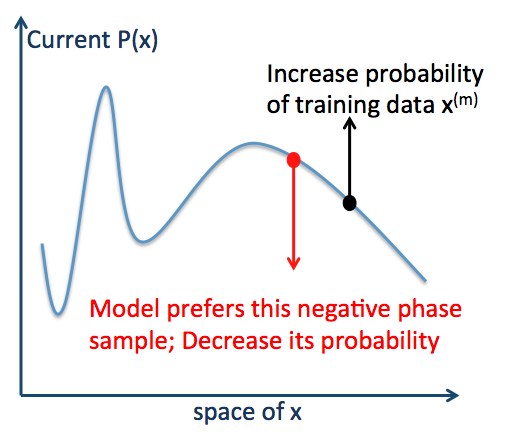
\includegraphics[scale=0.4]{figs/contrastive_divergence}}
\end{frame}


%%%%%%%%
\begin{frame}
\frametitle{Distributed Representations learned by RBM}
\bi
\item Vector $h$ act as \textbf{Distributed Representation} of data 
	\bi
	\item Multiple $h_j$ may be active simultaneously for a given $x$. (Multi-clustering)
	\item $2^{|h|}$ possible representations with $|h|\times|x|$ parameters. 
	\ei
\begin{center}
\scalebox{0.8}{
\begin{tikzpicture}[-,>=stealth',shorten >=1pt,auto,node distance=3cm,
  thick,main node/.style={circle,fill=blue!20,draw,font=\sffamily\Large\bfseries}]

  \node[main node] (x1) at (0,0) {$x_1$};
  \node[main node] (x2) at (2,0) {$x_2$};
  \node[main node] (x3) at (4,0) {$x_3$};
  \node[main node] (h1) at (0,2) {$h_1$};
  \node[main node] (h2) at (2,2) {$h_2$};
  \node[main node] (h3) at (4,2) {$h_3$};

  \path[every node/.style={font=\sffamily\small}]
    (x1) edge node {} (h1)
    (x1) edge node {} (h2)
    (x1) edge node {} (h3)
    (x2) edge node {} (h1)
    (x2) edge node {} (h2)
    (x2) edge node {} (h3)
    (x3) edge node {} (h1)
    (x3) edge node {} (h2)
    (x3) edge node {} (h3);
\end{tikzpicture}
}
\end{center}

\pause
\item A mixture model $p(x)=\sum_h p(c)p(x|c)$ would need $2^{|h|} \times |x|$ parameters:

\begin{center}
\scalebox{0.8}{
\begin{tikzpicture}[<-,>=stealth',shorten >=1pt,auto,node distance=3cm,
  thick,main node/.style={circle,fill=blue!20,draw,font=\sffamily\Large\bfseries}]

  \node[main node] (x1) at (0,0) {$x_1$};
  \node[main node] (x2) at (2,0) {$x_2$};
  \node[main node] (x3) at (4,0) {$x_3$};
  \node[main node] (h1) at (2,2) {$c$};
  

  \path[every node/.style={font=\sffamily\small}]
    (x1) edge node {} (h1)
    (x2) edge node {} (h1)
    (x3) edge node {} (h1);
\end{tikzpicture}
}
\end{center}


\ei
\end{frame}

%%%%%
\begin{frame}
\frametitle{Layer-wise Pre-training of RBMs}
\begin{columns}
\begin{column}{0.5\textwidth}
\begin{center}
\scalebox{0.8}{
\begin{tikzpicture}[-,>=stealth',shorten >=1pt,auto,node distance=3cm,
  thick,main node/.style={circle,fill=blue!20,draw,font=\sffamily\Large\bfseries}]

  \node[main node] (x1) at (0,0) {$x_1$};
  \node[main node] (x2) at (2,0) {$x_2$};
  \node[main node] (x3) at (4,0) {$x_3$};
  \node[main node] (h1) at (0,2) {$h_1$};
  \node[main node] (h2) at (2,2) {$h_2$};
  \node[main node] (h3) at (4,2) {$h_3$};
  \node[main node] (h'1) at (0,4) {$h'_1$};
  \node[main node] (h'2) at (2,4) {$h'_2$};
  \node[main node] (h'3) at (4,4) {$h'_3$};
  \node[main node] (h''1) at (0,6) {$h''_1$};
  \node[main node] (h''2) at (2,6) {$h''_2$};
  \node[main node] (h''3) at (4,6) {$h''_3$};
  \node at (5.1,1) {Layer1 RBM};
  \node at (5.1,3) {Layer2 RBM};
  \node at (5.1,5) {Layer3 RBM};

    \path[every node/.style={font=\sffamily\small}]
    (x1) edge node {} (h1)
    (x1) edge node {} (h2)
    (x1) edge node {} (h3) 
    (x2) edge node {} (h1)
    (x2) edge node {} (h2)
    (x2) edge node {} (h3) 
    (x3) edge node {} (h1)
    (x3) edge node {} (h2)
    (x3) edge node {} (h3)
    (h1) edge node {} (h'1)
    (h1) edge node {} (h'2)
    (h1) edge node {} (h'3)
    (h2) edge node {} (h'1)
    (h2) edge node {} (h'2)
    (h2) edge node {} (h'3)
    (h3) edge node {} (h'1)
    (h3) edge node {} (h'2)
    (h3) edge node {} (h'3)
    (h'1) edge node {} (h''1)
    (h'1) edge node {} (h''2)
    (h'1) edge node {} (h''3)
    (h'2) edge node {} (h''1)
    (h'2) edge node {} (h''2)
    (h'2) edge node {} (h''3)
    (h'3) edge node {} (h''1)
    (h'3) edge node {} (h''2)
    (h'3) edge node {} (h''3)
    ;

\end{tikzpicture}
}
\end{center}
\end{column}
\begin{column}{0.4\textwidth}
\be
\item Train Layer 1 RBM\\max $\log P(x,h)$
\item Train Layer 2 RBM\\max $\log P(h,h')$
\item Train Layer 3 RBM\\max $\log P(h',h'')$
\ee
\end{column}
\end{columns}
\end{frame}

%%%%%
\begin{frame}
\frametitle{Deep Belief Nets (DBN) =  Stacked RBM \cite{hinton06dbn}}
\begin{columns}
\begin{column}{0.4\textwidth}
\begin{center}
\scalebox{0.8}{
\begin{tikzpicture}[-,>=stealth',shorten >=1pt,auto,node distance=3cm,
  thick,main node/.style={circle,fill=blue!20,draw,font=\sffamily\Large\bfseries}]

  \node[main node] (x1) at (0,0) {$x_1$};
  \node[main node] (x2) at (2,0) {$x_2$};
  \node[main node] (x3) at (4,0) {$x_3$};
  \node[main node] (h1) at (0,2) {$h_1$};
  \node[main node] (h2) at (2,2) {$h_2$};
  \node[main node] (h3) at (4,2) {$h_3$};
  \node[main node] (h'1) at (0,4) {$h'_1$};
  \node[main node] (h'2) at (2,4) {$h'_2$};
  \node[main node] (h'3) at (4,4) {$h'_3$};
  \node[main node] (h''1) at (0,6) {$h''_1$};
  \node[main node] (h''2) at (2,6) {$h''_2$};
  \node[main node] (h''3) at (4,6) {$h''_3$};
  \node at (4.6,1) {Layer1};
  \node at (4.6,3) {Layer2};
  \node at (4.6,5) {Layer3};


  \path[<-,every node/.style={font=\sffamily\small}]
    (x1) edge node {} (h1)
    (x1) edge node {} (h2)
    (x1) edge node {} (h3) 
    (x2) edge node {} (h1)
    (x2) edge node {} (h2)
    (x2) edge node {} (h3) 
    (x3) edge node {} (h1)
    (x3) edge node {} (h2)
    (x3) edge node {} (h3)
    (h1) edge node {} (h'1)
    (h1) edge node {} (h'2)
    (h1) edge node {} (h'3)
    (h2) edge node {} (h'1)
    (h2) edge node {} (h'2)
    (h2) edge node {} (h'3)
    (h3) edge node {} (h'1)
    (h3) edge node {} (h'2)
    (h3) edge node {} (h'3);
    
    \path[every node/.style={font=\sffamily\small}]
    (h'1) edge node {} (h''1)
    (h'1) edge node {} (h''2)
    (h'1) edge node {} (h''3)
    (h'2) edge node {} (h''1)
    (h'2) edge node {} (h''2)
    (h'2) edge node {} (h''3)
    (h'3) edge node {} (h''1)
    (h'3) edge node {} (h''2)
    (h'3) edge node {} (h''3)
    ;

\end{tikzpicture}
}
\end{center}
\end{column}
\begin{column}{0.6\textwidth}
\bi
\item After pre-training, stacked RBM can be converted to DBN, defined as: $p(x)=\sum_{h,h',h''}p(x|h)p(h|h')p(h',h'')$\pause
\item This is a probabilistic generative model: Can sample from RBM at Layer3, then generate data $x$ via directed sigmoids \pause
\item Upper layers can be viewed as prior; More layers = better prior
\ei
\end{column}
\end{columns}
\end{frame}


%%%%%
\begin{frame}
\frametitle{Popular alternative: Initialize MLP with RBMs}
\begin{columns}
\begin{column}{0.4\textwidth}
\begin{center}
\scalebox{0.8}{
\begin{tikzpicture}[-,>=stealth',shorten >=1pt,auto,node distance=3cm,
  thick,main node/.style={circle,fill=blue!20,draw,font=\sffamily\Large\bfseries}]

  \node[main node] (x1) at (0,0) {$x_1$};
  \node[main node] (x2) at (2,0) {$x_2$};
  \node[main node] (x3) at (4,0) {$x_3$};
  \node[main node] (h1) at (0,2) {$h_1$};
  \node[main node] (h2) at (2,2) {$h_2$};
  \node[main node] (h3) at (4,2) {$h_3$};
  \node[main node] (h'1) at (0,4) {$h'_1$};
  \node[main node] (h'2) at (2,4) {$h'_2$};
  \node[main node] (h'3) at (4,4) {$h'_3$};
  \node[main node] (h''1) at (0,6) {$h''_1$};
  \node[main node] (h''2) at (2,6) {$h''_2$};
  \node[main node] (h''3) at (4,6) {$h''_3$};
  \node at (4.6,1) {Layer1};
  \node at (4.6,3) {Layer2};
  \node at (4.6,5) {Layer3};
  \node[main node] (y) at (2,8) {$y$};

  \path[->,every node/.style={font=\sffamily\small}]
    (x1) edge node {} (h1)
    (x1) edge node {} (h2)
    (x1) edge node {} (h3) 
    (x2) edge node {} (h1)
    (x2) edge node {} (h2)
    (x2) edge node {} (h3) 
    (x3) edge node {} (h1)
    (x3) edge node {} (h2)
    (x3) edge node {} (h3)
    (h1) edge node {} (h'1)
    (h1) edge node {} (h'2)
    (h1) edge node {} (h'3)
    (h2) edge node {} (h'1)
    (h2) edge node {} (h'2)
    (h2) edge node {} (h'3)
    (h3) edge node {} (h'1)
    (h3) edge node {} (h'2)
    (h3) edge node {} (h'3);
    
    \path[->,every node/.style={font=\sffamily\small}]
    (h'1) edge node {} (h''1)
    (h'1) edge node {} (h''2)
    (h'1) edge node {} (h''3)
    (h'2) edge node {} (h''1)
    (h'2) edge node {} (h''2)
    (h'2) edge node {} (h''3)
    (h'3) edge node {} (h''1)
    (h'3) edge node {} (h''2)
    (h'3) edge node {} (h''3)
    ;

    \path[->,every node/.style={font=\sffamily\small}]
    (h''1) edge node {} (y)
    (h''2) edge node {} (y)
    (h''3) edge node {} (y)
    ;

\end{tikzpicture}
}
\end{center}
\end{column}
\begin{column}{0.6\textwidth}
\bi
\item {Stacked RBMs can be used to initialize a Deep Neural Network (DNN), i.e. MLP}
\item {Then, fine-tuned by back-propagation}
\ei
\end{column}
\end{columns}
\end{frame}



%%%%%%%%%%%%%
\begin{frame}
\frametitle{What a Deep Generative Model can do}
After training on 20k images, the generative model of \cite{salakhutdinov09dbm}* can generate random images (dimension=8976) that are amazingly realistic!
\vspace{1cm} 
\centerline{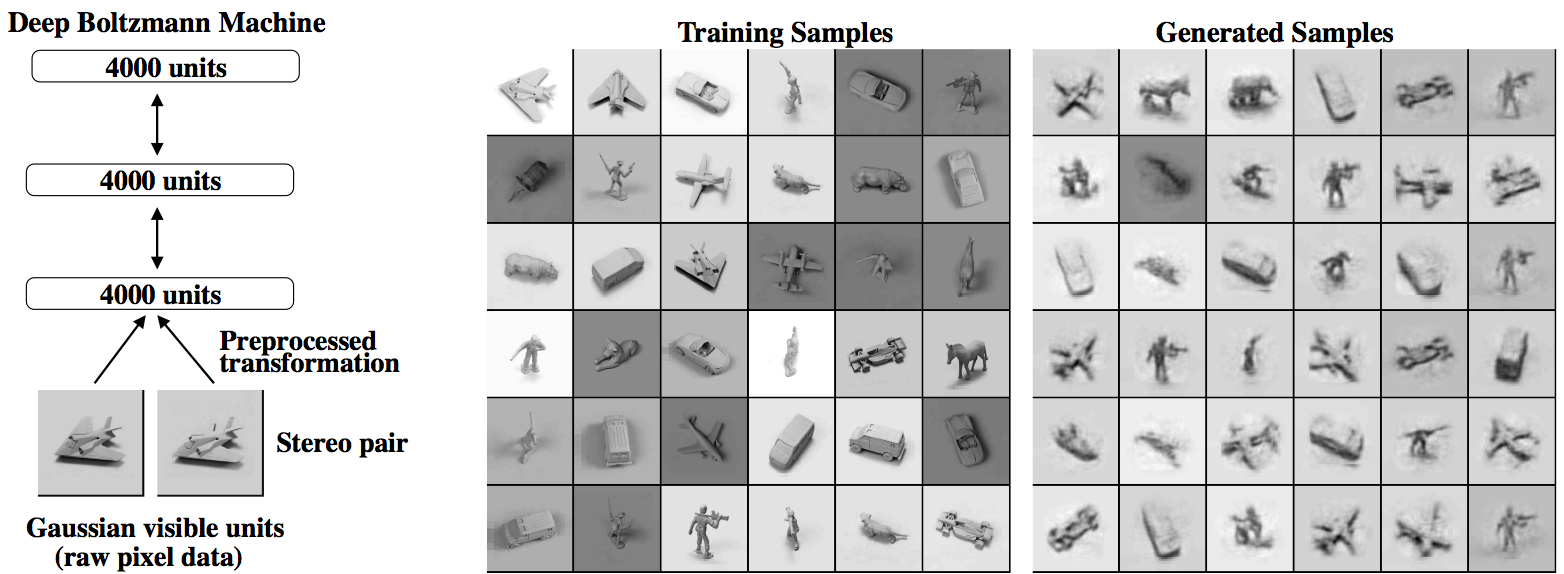
\includegraphics[scale=0.17]{figs/dbm_generation}}
\blfootnote{This model is a Deep Boltzmann Machine (DBM), different from Deep Belief Nets (DBN) but also built by stacking RBMs.}
\end{frame}

%%%%%%%%%%%%%
\begin{frame}
\frametitle{RBM and DBN Summary}
\be
\item Layer-wise pre-training is the innovation that rekindled interest in deep architectures. \pause
\item Pre-training focuses on optimizing likelihood on the data, not label. First model $p(x)$ to do better $p(y|x)$. \pause
\item Why RBM? $p(h|x)$ is tractable, so it's easy to stack.\pause
\item RBM training can be expensive. Solution: contrastive divergence\pause
\item We can stack RBMs to form a deep probabilistic generative model (DBN), or to initialize deep neural network (DNN) 
\ee
\end{frame}


%%%%%%%%%
\subsection[Auto-Encoders]{Auto-Encoders}

\begin{frame}
\frametitle{Auto-Encoders: Efficient replacement for RBM}

\begin{center}
\begin{tikzpicture}[->,>=stealth',shorten >=1pt,auto,node distance=3cm,
  thick,main node/.style={circle,fill=blue!20,draw,font=\sffamily\Large\bfseries}]

  \node[main node] (x1) at (0,0) {$x_1$};
  \node[main node] (x2) at (2,0) {$x_2$};
  \node[main node] (x3) at (4,0) {$x_3$};
  \node[main node] (h1) at (1,2) {$h_1$};
  \node[main node] (h2) at (3,2) {$h_2$};
  \node[main node] (h'1) at (0,4) {$x'_1$};
  \node[main node] (h'2) at (2,4) {$x'_2$};
  \node[main node] (h'3) at (4,4) {$x'_3$};
  \node at (7,1) {Encoder: $h =\sigma(Wx+b)$ };
  \node at (7,3) {Decoder: $x' =\sigma(W'h+d)$};


  \path[every node/.style={font=\sffamily\small}]
    (x1) edge node {} (h1)
    (x1) edge node {} (h2)
    (x2) edge node {} (h1)
    (x2) edge node {} (h2)
    (x3) edge node {} (h1)
    (x3) edge node {} (h2)
    (h1) edge node {} (h'1)
    (h1) edge node {} (h'2)
    (h1) edge node {} (h'3)
    (h2) edge node {} (h'1)
    (h2) edge node {} (h'2)
    (h2) edge node {} (h'3);

\end{tikzpicture}
\end{center}
\pause
Encourage $h$ to give small reconstruction error:
	\bi
	\item $Loss = \sum_m || x^{(m)} - DECODER(ENCODER(x^{(m)})) ||^2 $\pause
	\item Reconstruction: $x' =\sigma(W'\sigma(Wx+b)+d)$\pause
	\item $|h|$ is small to enforce "compression" of data \pause
	\item Back-prop for 2-layer nets, with $x^{(m)}$ as input \& output
	\ei
\end{frame}



%%%%%%%%%
\begin{frame}
\frametitle{Stacked Auto-Encoders (SAE) \cite{bengio06greedy}}
\bi 
\item The encoder/decoder gives same form $p(h|x)$, $p(x|h)$ as RBMs, so can be stacked in the same way
\pause
\begin{center}
\scalebox{0.65}{\begin{tikzpicture}[->,>=stealth',shorten >=1pt,auto,node distance=3cm,
  thick,main node/.style={circle,fill=blue!20,draw,font=\sffamily\Large\bfseries}]

  \node[main node] (x1) at (0,0) {$x_1$};
  \node[main node] (x2) at (2,0) {$x_2$};
  \node[main node] (x3) at (4,0) {$x_3$};
  \node[main node] (x4) at (6,0) {$x_4$};
  \node[main node] (h1) at (1,2) {$h_1$};
  \node[main node] (h2) at (3,2) {$h_2$};
  \node[main node] (h3) at (5,2) {$h_3$};
  \node[main node] (h'1) at (2,4) {$h'_1$};
  \node[main node] (h'2) at (4,4) {$h'_2$};
  \node[main node] (y) at (3,6) {$y$};
  \node at (7,1) {Layer1 Encoder};
  \node at (7,3) {Layer2 Encoder};
  \node at (7,5) {Output layer};


  \path[every node/.style={font=\sffamily\small}]
    (x1) edge node {} (h1)
    (x1) edge node {} (h2)
    (x1) edge node {} (h3)
    (x2) edge node {} (h1)
    (x2) edge node {} (h2)
    (x2) edge node {} (h3)
    (x3) edge node {} (h1)
    (x3) edge node {} (h2)
    (x3) edge node {} (h3)
    (x4) edge node {} (h1)
    (x4) edge node {} (h2)
    (x4) edge node {} (h3)
    (h1) edge node {} (h'1)
    (h1) edge node {} (h'2)
    (h2) edge node {} (h'1)
    (h2) edge node {} (h'2)
    (h3) edge node {} (h'1)
    (h3) edge node {} (h'2)
    (h'1) edge node {} (y)
    (h'2) edge node {} (y)
  
    ;
\end{tikzpicture}}
\end{center}

\pause
\item Unlike RBMs, Auto-encoders are deterministic. 
	\bi
	\item $h =\sigma(Wx+b)$, not $p(h=1) =\sigma(Wx+b)$\pause
	\item Disadvantage: Can't form deep generative model
	\item Advantage: Fast to train, useful still for DNN init
	\ei
\item Note similarities to RBM contrastive divergence 
\ei

\end{frame}


\begin{frame}
\frametitle{Variants: e.g. Denoising Auto-Encoder}

\begin{center}
\begin{tikzpicture}[->,>=stealth',shorten >=1pt,auto,node distance=3cm,
  thick,main node/.style={circle,fill=blue!20,draw,font=\sffamily\Large\bfseries}]

  \node[main node] (x1) at (0,0) {$\tilde{x_1}$};
  \node[main node] (x2) at (2,0) {$\tilde{x_2}$};
  \node[main node] (x3) at (4,0) {$\tilde{x_3}$};
  \node[main node] (h1) at (1,2) {$h_1$};
  \node[main node] (h2) at (3,2) {$h_2$};
  \node[main node] (h'1) at (0,4) {$x'_1$};
  \node[main node] (h'2) at (2,4) {$x'_2$};
  \node[main node] (h'3) at (4,4) {$x'_3$};
  \node at (7,0) {$\tilde{x} = x + $ noise};
  \node at (7,1) {Encoder: $h =\sigma(W\tilde{x}+b)$ };
  \node at (7,3) {Decoder: $x' =\sigma(W'h+d)$};


  \path[every node/.style={font=\sffamily\small}]
    (x1) edge node {} (h1)
    (x1) edge node {} (h2)
    (x2) edge node {} (h1)
    (x2) edge node {} (h2)
    (x3) edge node {} (h1)
    (x3) edge node {} (h2)
    (h1) edge node {} (h'1)
    (h1) edge node {} (h'2)
    (h1) edge node {} (h'3)
    (h2) edge node {} (h'1)
    (h2) edge node {} (h'2)
    (h2) edge node {} (h'3)
    ;

\end{tikzpicture}
\end{center}

\be
\item Perturb input data $x$ to $\tilde{x}$ using invariance from domain knowledge. 
\item Train weights to reduce reconstruction error with respect to original input: $||x-x'||$
\ee
\end{frame}


\begin{frame}
\frametitle{Denoising Auto-Encoders}
\bi
\item Example: Randomly shift, rotate, and scale input image
\item An image of "2" is a "2" no matter how you add noise, so the auto-encoder will try to cancel the variations that are not important. 
\ei
\centerline{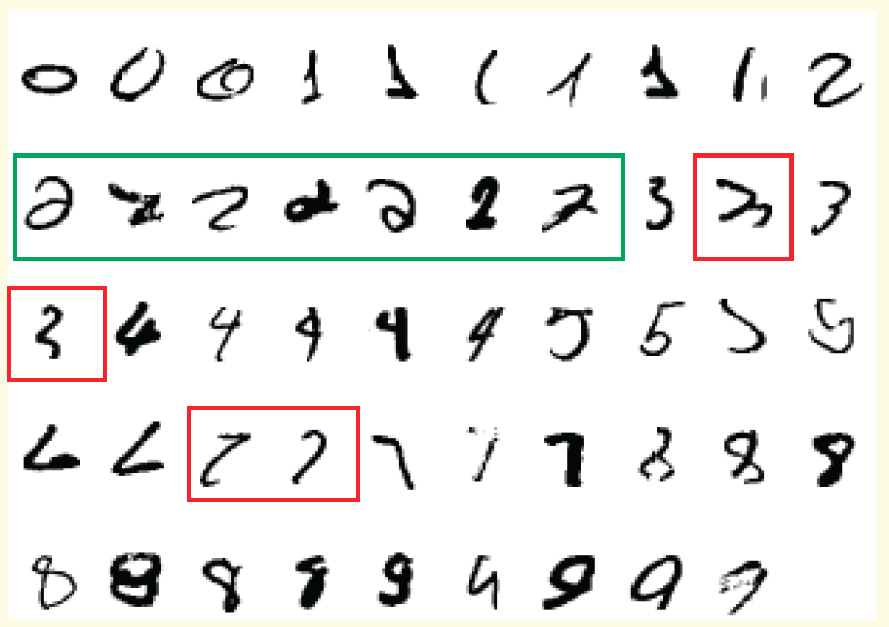
\includegraphics[scale=0.19]{figs/digit2}}
\blfootnote{Figure from Geoff Hinton's 2012 Coursera course, lecture 1: \url{https://www.coursera.org/course/neuralnets}}
\end{frame}

%%%%%%%%%%%%%%%%%%%%%%%%%%%%%%%%%%%%%%
\begin{frame}
\frametitle{Stacked Auto-Encoders (SAE): Summary}
\be
\item Auto-Encoders are cheaper alternatives to RBMs.
	\bi
	\item Not probabilistic, but fast to train using Backpropagation
	\item Achieves similar accuracies as RBM \cite{bengio06greedy}
	\ei
\pause
\item Auto-Encoders learn to "compress" and "re-construct" input data. Again, the focus is on modeling $p(x)$ first.  \pause
\item Many variants, some provide ways to incorporate domain knowledge.
\ee
\end{frame}


%%%%%%%%%
\subsection[Recurrent Units]{Recurrent Units}

\begin{frame}
\frametitle{Modeling sequence data}
\centerline{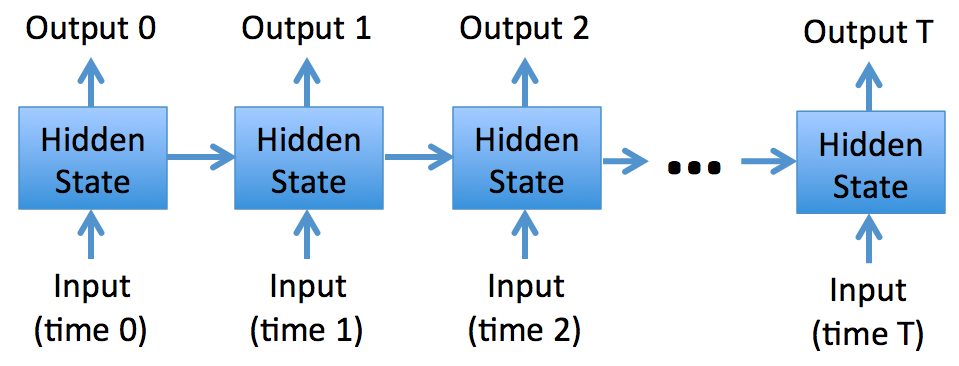
\includegraphics[scale=0.3]{figs/sequencemodel}}
\bi
\pause
\item Example applications:
  
	\bi 
        \item Time-series prediction
        \item Sequence-to-sequence transduction
	\item Language modeling $P(current\_word \mid previous\_words)$
	\ei
\ei
\end{frame}


\begin{frame}
\frametitle{Recurrent Neural Net Language Models}
Model $p(current\_word|previous\_words)$ with a recurrent hidden layer \cite{mikolov10rnnlm}

\begin{columns}
\column{0.6\textwidth}
\scalebox{0.6}{\begin{tikzpicture}[->,>=stealth',shorten >=1pt,auto,node distance=3cm,
  thick,main node/.style={circle,fill=blue!20,draw,font=\sffamily\Large\bfseries}]

  \node[main node] (x1) at (0,0) {$x_1$};
  \node[main node] (x2) at (2,0) {$x_2$};
  \node[main node] (x3) at (4,0) {$x_3$};
  \node[main node] (x4) at (6,0) {$x_4$};
  \node[main node] (x5) at (8,0) {$x_5$};
  \node[main node] (h1) at (4,2) {$h_1$};
  \node[main node] (h2) at (6,2) {$h_2$};
  \node[main node] (h'1) at (0,4) {$y_1$};
  \node[main node] (h'2) at (2,4) {$y_2$};
  \node[main node] (h'3) at (4,4) {$y_3$};

  \draw[blue,ultra thick,-latex,<->] (0,-1) -- node[]{Previous Word} (4,-1);
  \draw[blue,ultra thick,-latex,<->] (6,-1) -- node[]{Previous $h$} (8,-1);
  \draw[blue,ultra thick,-latex,<->] (0,5) -- node[]{Current Word (assume 3-word vocabulary)} (4,5);

   \node(wij) at (1,1) {$w_{ij}$};
   \node(wjk) at (1,3) {$w_{jk}$};

  \path[every node/.style={font=\sffamily\small}]
    (x1) edge node {} (h1)
    (x2) edge node {} (h1)
    (x3) edge node {} (h1)
    (x4) edge node {} (h1)
    (x5) edge node {} (h1)
    (x1) edge node {} (h2)
    (x2) edge node {} (h2)
    (x3) edge node {} (h2)
    (x4) edge node {} (h2)
    (x5) edge node {} (h2)
    (h1) edge node {} (h'1)
    (h2) edge node {} (h'1)
    (h1) edge node {} (h'2)
    (h2) edge node {} (h'2)
    (h1) edge node {} (h'3)
    (h2) edge node {} (h'3)
    ;
\end{tikzpicture}}
    \column{.4\textwidth}
\bi
\item Probability of word: $y_k=\frac{\exp(W_{jk}^T h)}{\sum_{k'}\exp(W_{jk'}^T h)}$
\item $[x_4,x_5]$ is a copy of $[h_1,h_2]$ from the previous time-step
\item $h_j=\sigma(W_{ij}^T x_i)$ is hidden state of partial sentence
\item Arbitrarily-long history is (theoretically) kept through recurrence
\ei
\end{columns}
\end{frame}

\begin{frame}
\frametitle{Training: Backpropagation through Time}
Unroll the hidden states for a few time-steps, then backprop.\\
{\color{red} Very deep network: vanishing/exploding gradients!}

\scalebox{0.8}{\begin{tikzpicture}[->,>=stealth',shorten >=1pt,auto,node distance=3cm,
  thick,main node/.style={circle,fill=blue!20,draw,font=\sffamily\Large\bfseries}]

  \node[main node] (x1) at (0,0) {$x_1$};
  \node[main node] (x2) at (2,0) {$x_2$};
  \node[main node] (x3) at (4,0) {$x_3$};
  \node[main node] (x4) at (6,0) {$h'_1$};
  \node[main node] (x5) at (8,0) {$h'_2$};
  \node[main node] (h1) at (4,2) {$h_1$};
  \node[main node] (h2) at (6,2) {$h_2$};
  \node[main node] (h'1) at (0,4) {$y_1$};
  \node[main node] (h'2) at (2,4) {$y_2$};
  \node[main node] (h'3) at (4,4) {$y_3$};

  \node[main node] (px1) at (2,-3) {$x_1$};
  \node[main node] (px2) at (4,-3) {$x_2$};
  \node[main node] (px3) at (6,-3) {$x_3$};
  \node[main node] (px4) at (8,-3) {$h''_1$};
  \node[main node] (px5) at (10,-3) {$h''_2$};

  \draw[blue,ultra thick,-latex,<->] (2,-4) -- node[]{"Input0" $[x_1,x_2,x_3]=[0,1,0]$} (6,-4);
  \draw[blue,ultra thick,-latex,<->] (0,-1) -- node[]{"Input1" $[x_1,x_2,x_3]=[1,0,0]$} (4,-1);
 \draw[blue,ultra thick,-latex,<->] (6,-1) -- node[]{Previous $h$} (8,-1);
\draw[blue,ultra thick,-latex,<->] (8,-4) -- node[]{Initial $h$} (10,-4);
   \node(wij) at (1,1) {$w_{ij}$};
   \node(wjk) at (1,3) {$w_{jk}$};
      \node(wij) at (3,-2) {$w_{ij}$};

  \path[every node/.style={font=\sffamily\small}]
    (px1) edge node {} (x4)
    (px2) edge node {} (x4)
    (px3) edge node {} (x4)
    (px4) edge node {} (x4)
    (px5) edge node {} (x4)
    (px1) edge node {} (x5)
    (px2) edge node {} (x5)
    (px3) edge node {} (x5)
    (px4) edge node {} (x5)
    (px5) edge node {} (x5)
    (x1) edge node {} (h1)
    (x2) edge node {} (h1)
    (x3) edge node {} (h1)
    (x4) edge node {} (h1)
    (x5) edge node {} (h1)
    (x1) edge node {} (h2)
    (x2) edge node {} (h2)
    (x3) edge node {} (h2)
    (x4) edge node {} (h2)
    (x5) edge node {} (h2)
    (h1) edge node {} (h'1)
    (h2) edge node {} (h'1)
    (h1) edge node {} (h'2)
    (h2) edge node {} (h'2)
    (h1) edge node {} (h'3)
    (h2) edge node {} (h'3)
    ;
\end{tikzpicture}}
\end{frame}

%%%%%%%
\begin{frame}
\frametitle{A popular recurrent unit: LSTM}
Long Short-term Memory (LSTM): 
\bi
\item Idea: Shouldn't need to back-prop to beginning of history. Just keep a memory of important bits. \pause
\item Introduces memory cell ($c_t$), with input/output/forget gates to keep track of what to remember and when
\ei
\centerline{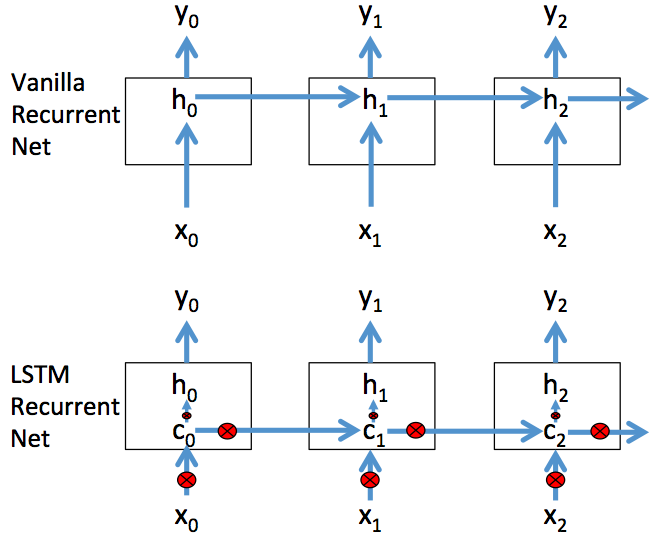
\includegraphics[scale=0.28]{figs/lstm_simpleschematic}}
\blfootnote{*Nice explanation of LSTM and variants here: \url{http://colah.github.io/posts/2015-08-Understanding-LSTMs/}}
\end{frame}

%%% 
\begin{frame}
\frametitle{LSTM in detail \cite{gers02peephole}}

\centerline{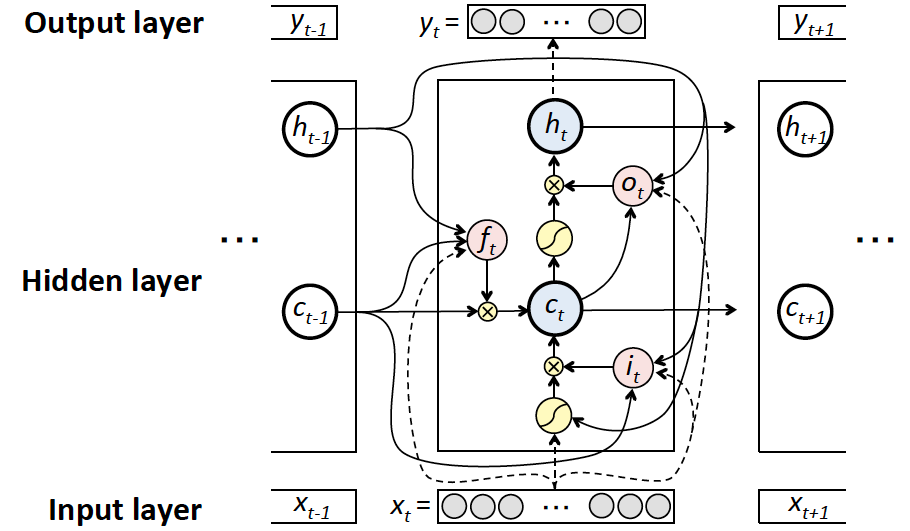
\includegraphics[scale=0.28]{figs/lstm_detailschematic}}
\vspace{-0.4cm}
\begin{eqnarray*}
  i_{t} &=&  \sigma (W_{xi} x_{t} + W_{ci} c_{t-1} + W_{hi} h_{t-1}) \\[-.25em]
  f_{t} &=&  \sigma (W_{xf} x_{t} + W_{cf} c_{t-1} + W_{hf} h_{t-1}) \\[-.25em]
  c_{t} &=&  f_{t} c_{t-1} + \!i_{t} \ tanh (W_{xc} x_{t} + W_{hc} h_{t-1}) \\[-.25em]
  o_{t} &=&  \sigma (W_{xo} x_{t} + W_{co} c_{t} + W_{ho} h_{t-1}) \\[-.25em]
  h_{t} &=&  o_{t} \tanh(c_{t}), \hspace{0.3cm}  y_{t} =  softmax(W_{hy} h_{t})
\end{eqnarray*}
\vspace{-0.2cm}
\blfootnote{Figure courtesy of Adhi Kuncoro \& Yuichiro Sawai}

\end{frame}




%%%%%%%%%
\subsection[Convolution]{Convolution} 

\begin{frame}
\frametitle{Convolution} % frame1
\begin{tikzpicture}[->,>=stealth',shorten >=1pt,auto,node distance=3cm,
  thick,main node/.style={circle,fill=blue!20,draw,font=\sffamily\Large\bfseries}]

  \node[main node] (x1) at (0,0) {$x_1$};
  \node[main node] (x2) at (2,0) {$x_2$};
  \node[main node] (x3) at (4,0) {$x_3$};
  \node[main node] (x4) at (6,0) {$x_4$};
  \node[main node] (x5) at (8,0) {$x_5$};
  \node[main node] (h1) at (2,2) {$h_1$};
  \node[main node] (h2) at (4,2) {$h_2$};
  \node[main node] (h3) at (6,2) {$h_3$};
  	
     \path[red,every node/.style={font=\sffamily\small}]
    (x1) edge node {} (h1)     ;
     \path[blue,every node/.style={font=\sffamily\small}]
    (x2) edge node {} (h1)     ;
   \path[yellow,every node/.style={font=\sffamily\small}]
    (x3) edge node {} (h1)     ;

\end{tikzpicture}
Sliding window of shared weights: $h_j = \sum_{\tau=0}^{2}w_{\tau}x_{j+\tau}$\\[0.2cm]
\end{frame}

%%%%%%%%%
\begin{frame}
\frametitle{Convolution} %frame2
\begin{tikzpicture}[->,>=stealth',shorten >=1pt,auto,node distance=3cm,
  thick,main node/.style={circle,fill=blue!20,draw,font=\sffamily\Large\bfseries}]

  \node[main node] (x1) at (0,0) {$x_1$};
  \node[main node] (x2) at (2,0) {$x_2$};
  \node[main node] (x3) at (4,0) {$x_3$};
  \node[main node] (x4) at (6,0) {$x_4$};
  \node[main node] (x5) at (8,0) {$x_5$};
  \node[main node] (h1) at (2,2) {$h_1$};
  \node[main node] (h2) at (4,2) {$h_2$};
  \node[main node] (h3) at (6,2) {$h_3$};
  
	
     \path[red,every node/.style={font=\sffamily\small}]
    (x2) edge node {} (h2)     ;
     \path[blue,every node/.style={font=\sffamily\small}]
    (x3) edge node {} (h2)     ;
   \path[yellow,every node/.style={font=\sffamily\small}]
    (x4) edge node {} (h2)     ;

\end{tikzpicture}
Sliding window of shared weights: $h_j = \sum_{\tau=0}^{2}w_{\tau}x_{j+\tau}$\\[0.2cm]
\end{frame}

%%%%%%%%%
\begin{frame}
\frametitle{Convolution} %frame3
\begin{tikzpicture}[->,>=stealth',shorten >=1pt,auto,node distance=3cm,
  thick,main node/.style={circle,fill=blue!20,draw,font=\sffamily\Large\bfseries}]

  \node[main node] (x1) at (0,0) {$x_1$};
  \node[main node] (x2) at (2,0) {$x_2$};
  \node[main node] (x3) at (4,0) {$x_3$};
  \node[main node] (x4) at (6,0) {$x_4$};
  \node[main node] (x5) at (8,0) {$x_5$};
  \node[main node] (h1) at (2,2) {$h_1$};
  \node[main node] (h2) at (4,2) {$h_2$};
  \node[main node] (h3) at (6,2) {$h_3$};
 	
     \path[red,every node/.style={font=\sffamily\small}]
    (x3) edge node {} (h3)     ;
     \path[blue,every node/.style={font=\sffamily\small}]
    (x4) edge node {} (h3)     ;
   \path[yellow,every node/.style={font=\sffamily\small}]
    (x5) edge node {} (h3)     ;

\end{tikzpicture}
Sliding window of shared weights: $h_j = \sum_{\tau=0}^{2}w_{\tau}x_{j+\tau}$\\[0.2cm]
\end{frame}

\begin{frame}
\frametitle{Convolution} % frame4
\begin{tikzpicture}[->,>=stealth',shorten >=1pt,auto,node distance=3cm,
  thick,main node/.style={circle,fill=blue!20,draw,font=\sffamily\Large\bfseries}]

  \node[main node] (x1) at (0,0) {$x_1$};
  \node[main node] (x2) at (2,0) {$x_2$};
  \node[main node] (x3) at (4,0) {$x_3$};
  \node[main node] (x4) at (6,0) {$x_4$};
  \node[main node] (x5) at (8,0) {$x_5$};
  \node[main node] (h1) at (2,2) {$h_1$};
  \node[main node] (h2) at (4,2) {$h_2$};
  \node[main node] (h3) at (6,2) {$h_3$};
  	
     \path[red,every node/.style={font=\sffamily\small}]
       (x1) edge node {} (h1)     
        (x2) edge node {} (h2)     
        (x3) edge node {} (h3)     ;

     \path[blue,every node/.style={font=\sffamily\small}]
       (x2) edge node {} (h1)     
        (x3) edge node {} (h2)     
        (x4) edge node {} (h3)     ;

   \path[yellow,every node/.style={font=\sffamily\small}]
      (x3) edge node {} (h1)     
       (x4) edge node {} (h2)     
       (x5) edge node {} (h3)     ;
\end{tikzpicture}
Sliding window of shared weights: $h_j = \sum_{\tau=0}^{2}w_{\tau}x_{j+\tau}$\\[0.2cm]
\end{frame}

\begin{frame}
\frametitle{Pooling} 
\begin{tikzpicture}[->,>=stealth',shorten >=1pt,auto,node distance=3cm,
  thick,main node/.style={circle,fill=blue!20,draw,font=\sffamily\Large\bfseries}]

  \node[main node] (x1) at (0,0) {$x_1$};
  \node[main node] (x2) at (2,0) {$x_2$};
  \node[main node] (x3) at (4,0) {$x_3$};
  \node[main node] (x4) at (6,0) {$x_4$};
  \node[main node] (x5) at (8,0) {$x_5$};
  \node[main node] (h1) at (2,2) {$h_1$};
  \node[main node] (h2) at (4,2) {$h_2$};
  \node[main node] (h3) at (6,2) {$h_3$};
  \node[main node] (p1) at (3,4) {$p_1$};
  \node[main node] (p2) at (5,4) {$p_2$};
  	
     \path[red,every node/.style={font=\sffamily\small}]
       (x1) edge node {} (h1)     
        (x2) edge node {} (h2)     
        (x3) edge node {} (h3)     ;

     \path[blue,every node/.style={font=\sffamily\small}]
       (x2) edge node {} (h1)     
        (x3) edge node {} (h2)     
        (x4) edge node {} (h3)     ;

   \path[yellow,every node/.style={font=\sffamily\small}]
      (x3) edge node {} (h1)     
       (x4) edge node {} (h2)     
       (x5) edge node {} (h3)     ;
     
     \path[every node/.style={font=\sffamily\small}]
       (h1) edge node {} (p1)     
        (h2) edge node {} (p1)     
        (h2) edge node {} (p2)  
        (h3) edge node {} (p2)    ;  
       
\end{tikzpicture}
Max-Pooling nodes: $p_1=max(h_1,h_2)$, $p_2=max(h_2,h_3)$\\[0.2cm]
Advantages of Convolution + Pooling:
\be
\item Fewer weights
\item Shift invariance
\ee
\end{frame}

\begin{frame}
\frametitle{Convolutional Nets in vision \cite{lecun98conv}}
\vspace{0.1cm}
\begin{columns}[c]
    \column{.5\textwidth}
\scalebox{0.55}{\begin{tikzpicture}[->,>=stealth',shorten >=1pt,auto,node distance=3cm,
  thick,main node/.style={circle,fill=blue!20,draw,font=\sffamily\Large\bfseries}]

  \node[main node] (x1) at (0,0) {$x_1$};
  \node[main node] (x2) at (2,0) {$x_2$};
  \node[main node] (x3) at (4,0) {$x_3$};
  \node[main node] (x4) at (6,0) {$x_4$};
  \node[main node] (x5) at (8,0) {$x_5$};
  \node[main node] (h1) at (2,2) {$h_1$};
  \node[main node] (h2) at (4,2) {$h_2$};
  \node[main node] (h3) at (6,2) {$h_3$};
  \node[main node] (h'1) at (3,4) {$p_1$};
  \node[main node] (h'2) at (5,4) {$p_2$};

  \path[every node/.style={font=\sffamily\small}]
    (x1) edge node {} (h1)
    (x2) edge node {} (h1)
    (x3) edge node {} (h1)
    (x2) edge node {} (h2)
    (x3) edge node {} (h2)
    (x4) edge node {} (h2)
    (x3) edge node {} (h3)
    (x4) edge node {} (h3)
    (x5) edge node {} (h3)
    (h1) edge node {} (h'1)
    (h2) edge node {} (h'1)
    (h2) edge node {} (h'2)
    (h3) edge node {} (h'2)
    ;
\end{tikzpicture}}
    \column{.5\textwidth}
{\bf Receptive Field (RF)}: each $h_j$ only connects to small input region via convolution.\\
{\bf Pooling}: e.g. $p_1=max(h_1,h_2)$ or $p_1=\sqrt{h_1^2+h_2^2}$\\[0.2cm]
\end{columns}
\pause
\begin{center}
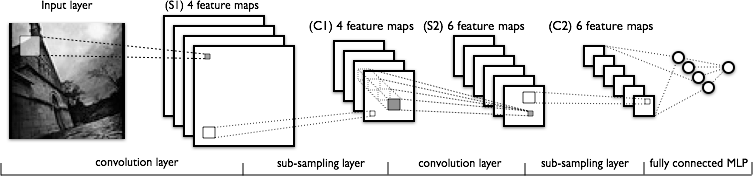
\includegraphics[scale=0.53]{figs/lenet}\\
\tiny{(Figure from \url{http://deeplearning.net/tutorial/lenet.html})}
\end{center}
\end{frame}


%%%%%
\begin{frame}
\frametitle{Section Summary}
\bi
\item RBM
\item Auto-Encoders
\item Recurrent Units
\item Convolution
\ei
\end{frame}


%%% 3. TRICKS
%SECTION%%%%%%%%%%%%%%%%%%%
\section[Tricks]{3. Tricks of the Trade}
\begin{frame}
\small{\frametitle{Outline}
\tableofcontents
}
\end{frame}
%%%%%%%%%%%%%%%%%%%%


%% SUBSECTION%%%%%
\subsection[Optimization]{Optimization: Making SGD work, Adaptive Learning Rate, 2nd-order methods}

%%%%%%
\begin{frame}
\frametitle{Neural Net Training Recipe}
\centerline{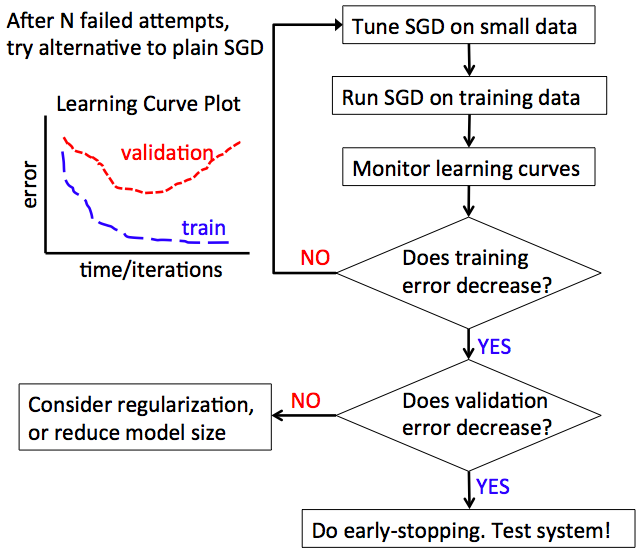
\includegraphics[scale=0.42]{figs/training_recipe}}
\end{frame}

%%%%%%
\begin{frame}
\frametitle{Making plain SGD Work}
\bi
\item With some tuning, SGD often works just as well as more advanced optimization methods! \pause
\item Important hyper-parameters: 
	\bi
	\item Learning rate: tune on small data first
	\item Mini-batch size: fit to computer's memory
	\ei 
	\pause
\item General tips:
	\bi
	\item Shuffle training data
	\item Scale training data within suitable range 
	\item Randomly initialize weights, e.g. uniform$[-1/\sqrt{(FanIn)}, 1/\sqrt{(FanIn)}]$
	\ei
\ei	
\end{frame}


%%%%%%%%%%%%%
\begin{frame}
\frametitle{Effect of Learning Rate $\gamma$ on SGD Convergence}
\bi
\item Update: $w \leftarrow w - \gamma( \sum_m {\color{red} Error^{(m)}} * {\color{blue} \sigma'(in^{(m)})} * x^{(m)
})$
\bi
        \item $\gamma$: try to be as large as possible without divergence.
        \item Common heuristic: $\gamma_t = \frac{\gamma_0}{1 + \gamma_0 * \lambda * t} = O(1/t)$ 
\ei
\item Analysis by \cite{schaul13learningrate} (in plot, $\eta \equiv \gamma$):
\ei
\centerline{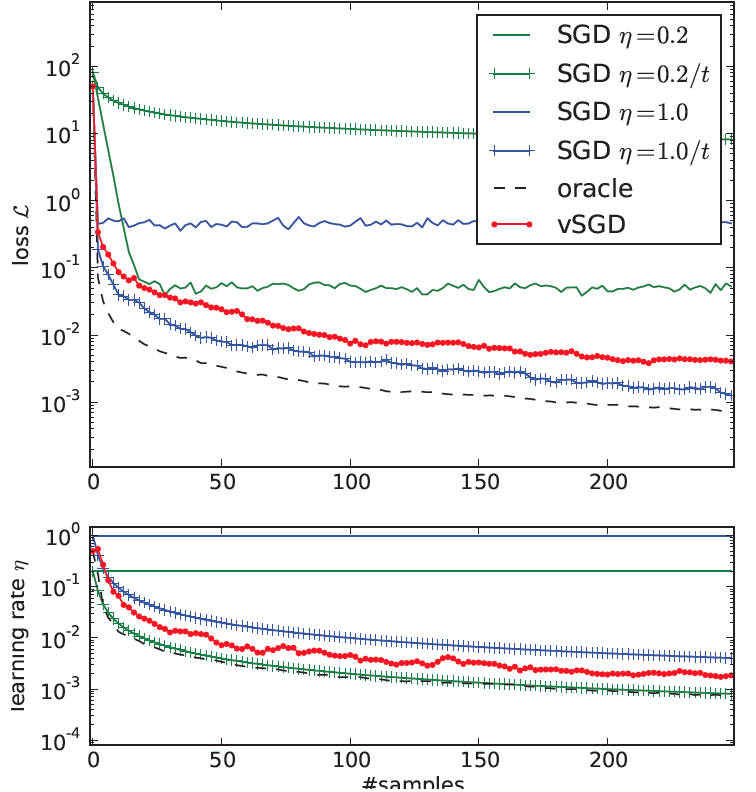
\includegraphics[scale=0.23]{figs/schaul13learningrate}}
\end{frame}


%%%%
\begin{frame}
\frametitle{Difficulty of optimizing highly non-convex loss functions}
\bi
\item "Pathological curvature" is tough to navigate for SGD 
\item Many methods for avoiding this zig-zag problem.
\ei
\centerline{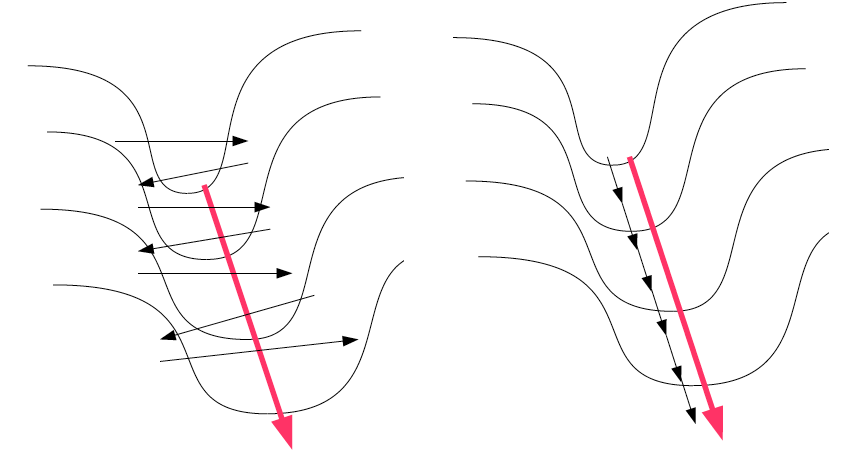
\includegraphics[scale=0.36]{figs/gradient_vs_newton}}
\blfootnote{Figure from \cite{martens10hessianfree}}
\end{frame}

%%%%%%
\begin{frame}
\frametitle{SGD + Momentum}
\bi
\item Idea: Accelerate in the direction that is consistently pointed to by successive gradients
\pause
\item Let update equation be: $w_{t+1} = w_t + \Delta w_t$
	\bi
	\item SGD: $\Delta w_t = -\gamma g_t$, where $g_t$ is gradient
	\pause
	\item SGD+Momemtum: $\Delta w_t = \rho \Delta w_{t-1} - \gamma g_t$ \pause
	\ei
\item $\rho$: a constant that determines how much momentum from previous updates \pause
\item Zig-zag directions will be cancelled out, while others will be accelerated.
\ei
\blfootnote{Note slight change of notation in this section: $w$ is a vector of weights, subscript $t$ in $w_t$ refers to weight at time $t$, not index as in previous sections}
\end{frame}

%%%%%%
\begin{frame}
\frametitle{Adaptive Learning Rate: ADAGRAD \cite{duchi11adagrad}}
\bi
\item Idea: 
	\bi 
	\item Each individual weight has it's own dynamic learning rate. 
	\item Weights with large derivative have smaller learning rate, weights with small derivative have large learning rate $\rightarrow$ different scales are balanced
	\ei
\item Let update equation be: $w_{t+1} = w_t + \Delta w_t$
	\bi
	\item SGD: $\Delta w_t = -\gamma g_t$, where $g_t$ is gradient
	\item ADAGRAD: $\Delta w_t = - \frac{\gamma}{diag(\sqrt{\sum_{\tau=1}^t g_\tau g_\tau^T})} g_t$
	\ei 
\item Denominator accumulates the $\ell_2$ norm of past gradients per dimension. 
\ei
\end{frame}

%%%%%%
\begin{frame}
\frametitle{Adaptive Learning Rate: ADADELTA \cite{zeiler12adadelta}}
\bi
\item Idea: Similar to ADAGRAD, but no learning rate.
	\bi
	\item ADAGRAD: $\Delta w_t = - \frac{\gamma}{diag(\sqrt{\sum_{\tau=1}^t g_\tau g_\tau^T})} g_t$
	\ei
\item ADADELTA: 
	\be
	\item Accumulate gradient over sliding window: $E[g^2]_t = \rho E[g^2]_{t-1} + (1-\rho) g_t g_t^T$\\[0.2cm]
	\item $\Delta w_t = - \frac{RMS(E[\Delta w]_{t-1})}{RMS(E[g^2]_t)} g_t$\\[0.2cm]
	 where $RMS(E[g^2]_t) = \sqrt{E[g^2]_t + \epsilon}$\\[0.2cm]
	\item Accumulate update over sliding window: $E[\Delta w^2]_t = \rho E[\Delta w^2]_{t-1} + (1-\rho) \Delta w_t \Delta w_t^T$
	\ee
\ei
\end{frame}

\begin{frame}
\frametitle{2nd-order (Newton) methods}
\bi
\item Idea: approximate the loss function locally with a quadratic\\[0.2cm]
$L(w+z) \approx q_w(z) \equiv L(w) + \nabla L(w)^T z + \frac{1}{2} z^T H z $\\[0.2cm]
\hspace{1cm} where $H$ is the Hessian (curvature matrix) at $w$\\[0.2cm]
\pause
\item Minimizing this gives the search direction: $z^{*}=-H^{-1}\nabla L(w) $
        \bi
        \item Intuitively, $H^{-1}$ fixes any pathological curvature for $\nabla L(w)$
        \item In practice, don't want to store nor invert $H$
        \ei
\pause
\item Quasi-Newton methods
        \bi
        \item L-BFGS: uses low-rank approximation of $H^{-1}$
        \pause
        \item Hessian-free (i.e. truncated Newton): (1) minimize $q_w(z)$ with conjugate gradient method; (2) computes $Hz$ directly using finite-difference: $Hz = \lim_{\epsilon\rightarrow 0} \frac{\nabla L(w+\epsilon z) - \nabla L(w)}{\epsilon}$
        \ei
\ei
\end{frame}

\begin{frame}
\frametitle{Hessian-free optimization results}
\bi
\item Experiments in \cite{martens10hessianfree} \\[0.2cm]
\begin{center}
(Random initialization + 2nd-order Hessian-free optimizer) \\[0.2cm]
 gives lower training error than \\[0.2cm]
 (Pre-training initialization + 1-order optimizer).\\[0.5cm]
 \end{center}
 \item Nice results in Recurrent Nets too \cite{martens11recurrent}
\ei
\end{frame}

%% SUBSECTION%%%%%
\subsection[Regularization]{Regularization: Dropout, Multi-task learning}


%%%%%%%%%%%%%%%%
\begin{frame}
\frametitle{Dropout \cite{hinton12dropout}}
\begin{columns}
\begin{column}{0.5\textwidth}
\bi
\item Each time we present $x^{(m)}$, randomly delete each hidden node with 0.5 probability
\item This is like sampling from $2^{|h|}$ different architectures
\item At test time, use all nodes but halve the weights
\item Effect: Reduce overfitting by preventing "co-adaptation"; ensemble model averaging
\ei
\end{column}
\begin{column}{0.5\textwidth}
\begin{center}
\begin{tikzpicture}[->,>=stealth',shorten >=1pt,auto,node distance=3cm,
  thick,main node/.style={circle,fill=blue!20,draw,font=\sffamily\Large\bfseries},cross/.style={path picture={
  \draw[red]
(path picture bounding box.south east) -- (path picture bounding box.north west) (path picture bounding box.south west) -- (path picture bounding box.north east);
}}]

 \node[main node] (x1) at (0,0) {$x_1$};
  \node[main node] (x2) at (2,0) {$x_2$};
  \node[main node] (x3) at (4,0) {$x_3$};
  \node[main node] (h1) at (0,2) {$h_1$};
  \node[main node] (h2) at (2,2) {$h_2$};
  \node[main node] (h3) at (4,2) {$h_3$};
  \node[main node] (h'1) at (0,4) {$h'_1$};
  \node[main node] (h'2) at (2,4) {$h'_2$};
  \node[main node] (h'3) at (4,4) {$h'_3$};
  \node[main node] (y) at (2,6) {$y$};
   \node [draw,circle,cross,minimum width=1 cm] at (0,2){};
   \node [draw,circle,cross,minimum width=1 cm] at (2,4){};
   \node [draw,circle,cross,minimum width=1 cm] at (4,4){};


  \path[every node/.style={font=\sffamily\small}]
    (x1) edge node {} (h1)
    (x1) edge node {} (h2)
    (x1) edge node {} (h3)
    (x2) edge node {} (h1)
    (x2) edge node {} (h2)
    (x2) edge node {} (h3)
    (x3) edge node {} (h1)
    (x3) edge node {} (h2)
    (x3) edge node {} (h3)
    (h1) edge node {} (h'1)
    (h1) edge node {} (h'2)
    (h1) edge node {} (h'3)
    (h2) edge node {} (h'1)
    (h2) edge node {} (h'2)
    (h2) edge node {} (h'3)
    (h3) edge node {} (h'1)
    (h3) edge node {} (h'2)
    (h3) edge node {} (h'3)
    
      (h'1) edge node {} (y)
    (h'2) edge node {} (y)
    (h'3) edge node {} (y) ;

\end{tikzpicture}
\end{center}
\end{column}
\end{columns}
\end{frame}

%%%%%%%%%%%%%%%%
\begin{frame}
\frametitle{Dropout \cite{hinton12dropout}}
\begin{columns}
\begin{column}{0.5\textwidth}
\bi
\item Each time we present $x^{(m)}$, randomly delete each hidden node with 0.5 probability
\item This is like sampling from $2^{|h|}$ different architectures
\item At test time, use all nodes but halve the weights
\item Effect: Reduce overfitting by preventing "co-adaptation"; ensemble model averaging
\ei
\end{column}
\begin{column}{0.5\textwidth}
\begin{center}
\begin{tikzpicture}[->,>=stealth',shorten >=1pt,auto,node distance=3cm,
  thick,main node/.style={circle,fill=blue!20,draw,font=\sffamily\Large\bfseries},cross/.style={path picture={
  \draw[red]
(path picture bounding box.south east) -- (path picture bounding box.north west) (path picture bounding box.south west) -- (path picture bounding box.north east);
}}]

 \node[main node] (x1) at (0,0) {$x_1$};
  \node[main node] (x2) at (2,0) {$x_2$};
  \node[main node] (x3) at (4,0) {$x_3$};
  \node[main node] (h1) at (0,2) {$h_1$};
  \node[main node] (h2) at (2,2) {$h_2$};
  \node[main node] (h3) at (4,2) {$h_3$};
  \node[main node] (h'1) at (0,4) {$h'_1$};
  \node[main node] (h'2) at (2,4) {$h'_2$};
  \node[main node] (h'3) at (4,4) {$h'_3$};
  \node[main node] (y) at (2,6) {$y$};
   \node [draw,circle,cross,minimum width=1 cm] at (0,2){};
   \node [draw,circle,cross,minimum width=1 cm] at (2,4){};
   \node [draw,circle,cross,minimum width=1 cm] at (4,4){};


  \path[every node/.style={font=\sffamily\small}]
    (x1) edge node {} (h2)
    (x1) edge node {} (h3)
    (x2) edge node {} (h2)
    (x2) edge node {} (h3)
    (x3) edge node {} (h2)
    (x3) edge node {} (h3)
    (h2) edge node {} (h'1)
    (h3) edge node {} (h'1)
      (h'1) edge node {} (y)
  ;

\end{tikzpicture}
\end{center}
\end{column}
\end{columns}
\end{frame}


\begin{frame}
\frametitle{Some Results: TIMIT phone recognition}
\centerline{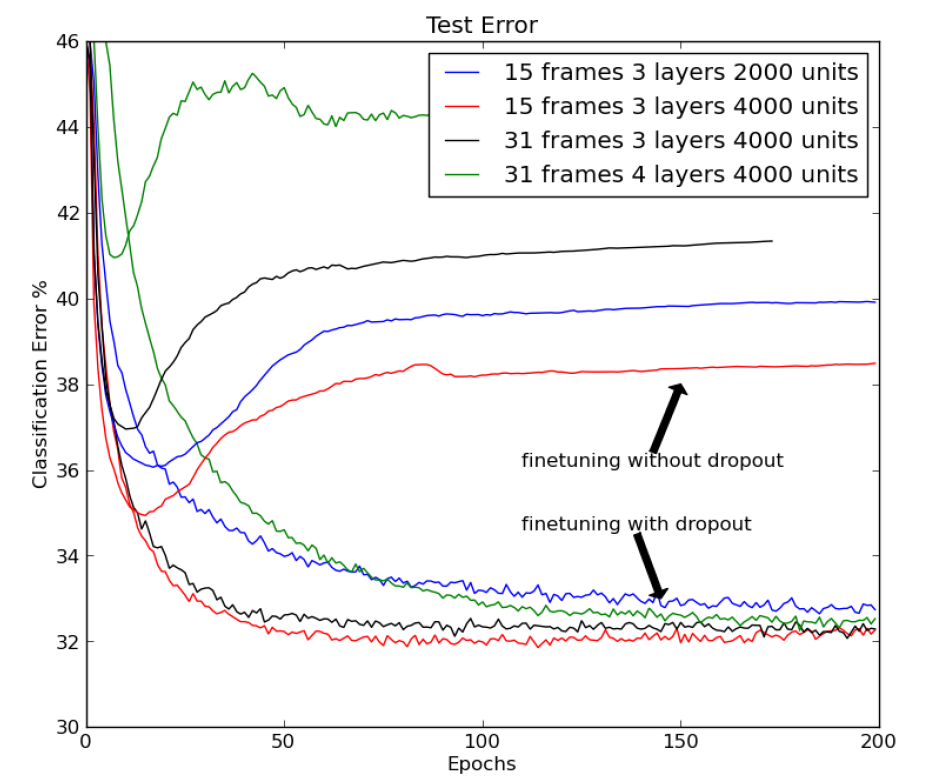
\includegraphics[scale=0.3]{figs/dropout_timit}}
\end{frame}

%%%%
\begin{frame}
\frametitle{Multi-task Learning: sharing hidden layers }
\bi
\item If too data is insufficient for desired task: 
\be
	\item train jointly with related tasks with shared hidden layer
	\item use related tasks' hidden layer as feature representation
\ee
\item e.g. \cite{liu15multitask}
\ei
\centerline{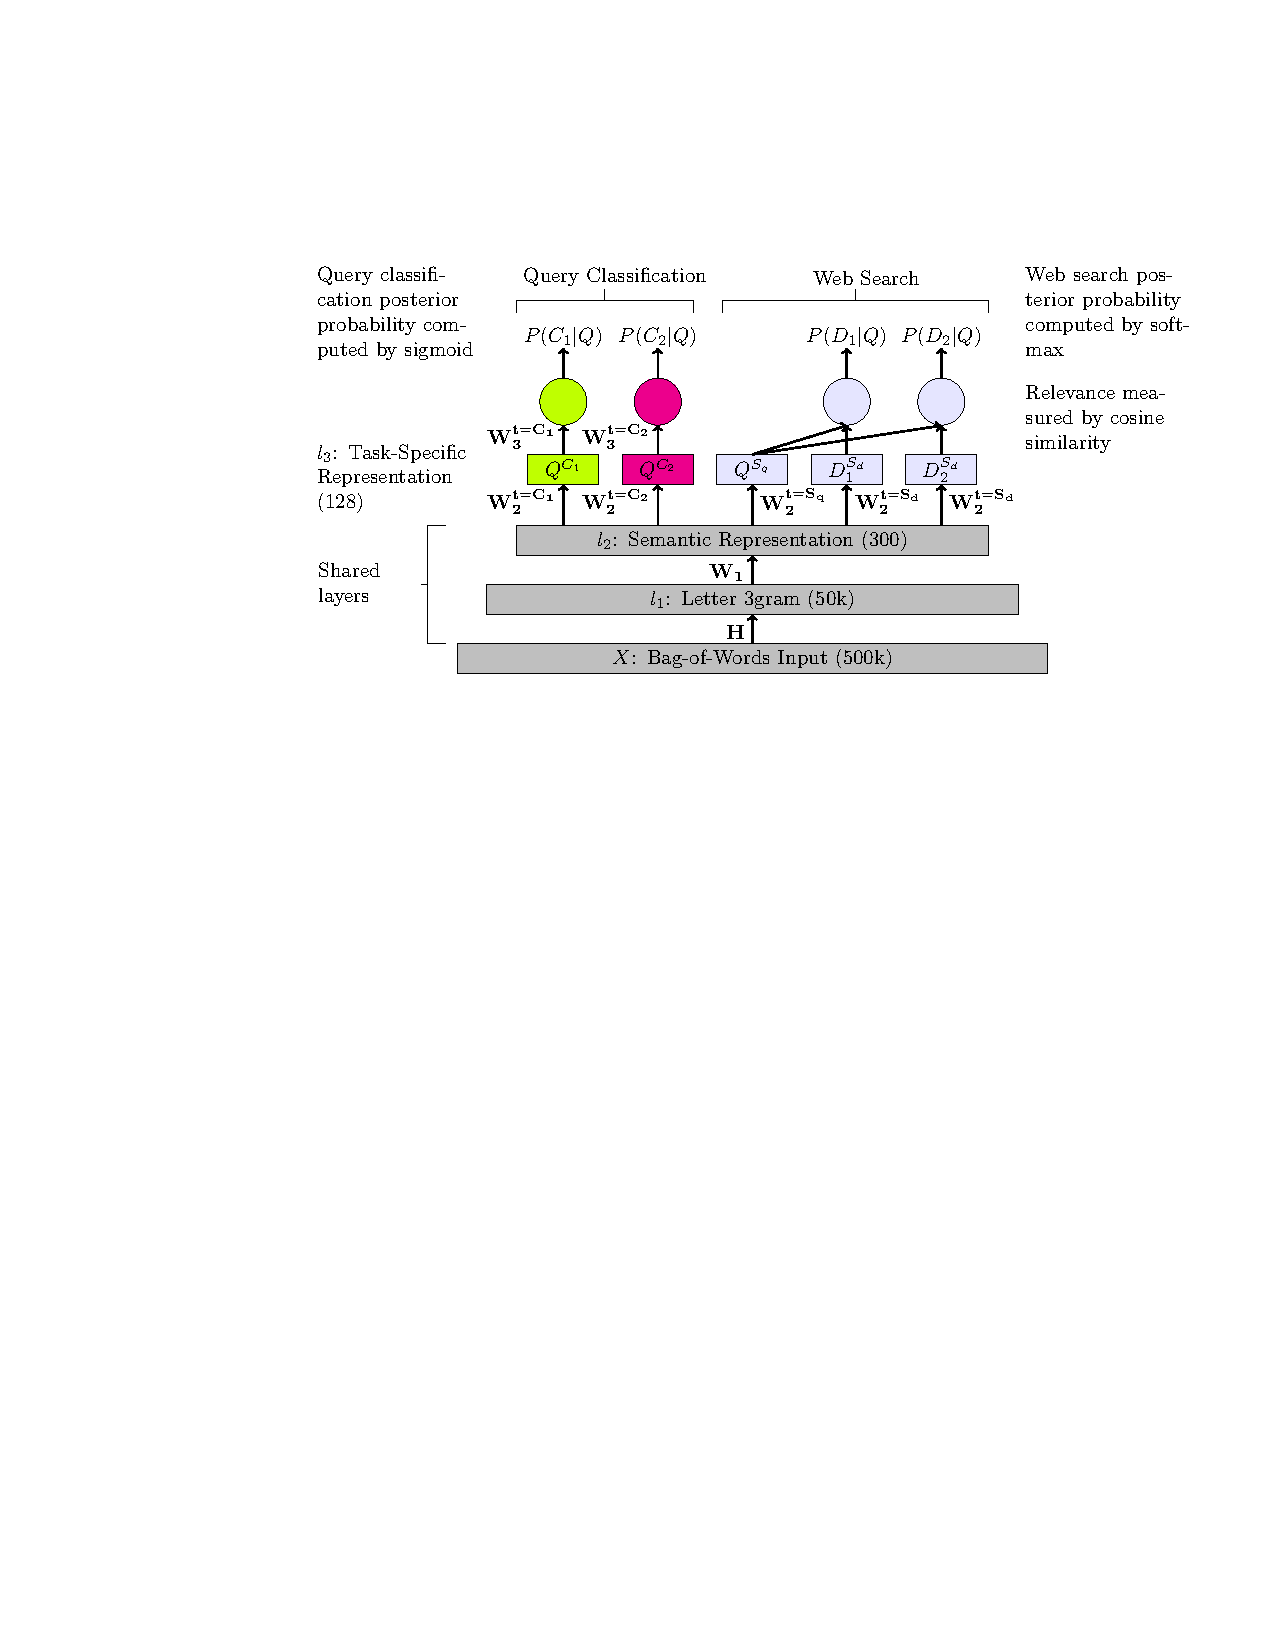
\includegraphics[scale=0.7]{figs/liu15multitask_mtdnn_arch}}
\blfootnote{See also \cite{caruana97,collobert11scratch,bordes12joint}}
\end{frame}

%%%%
\begin{frame}[plain]
\frametitle{Multi-task learning results in \cite{liu15multitask}}

\begin{table}
\centering
\tabcolsep=0.08cm
\begin{tabular}{|c | c | c | c | c || c | }
\hline
\multirow{2}{*}{Task}		&\multicolumn{4}{|c||}{Query Classification} & Web \\ \cline{2-5}
\multicolumn{1}{ |c| }{} 	&Restaurant	& Hotel  	&Flight		&Nightlife	  &Search\\ \hline \hline
Train							&1,585K		&2,131K	&1,880K	&1,214K	  &4M queries, click-through docs \\ \hline
Test									&3,074			&6,307		&6,199		&298		  &12K queries / 897K docs \\ \hline
\end{tabular}
\end{table}

1. Train jointly with all 5 tasks with shared hidden layer
\begin{table}[ht!]
\centering
\tabcolsep=0.09cm
\begin{tabular}{ l | c | c | c | c }
\hline
\multirow{2}{*}{Model}	&\multicolumn{4}{|c}{Query Classification (Accuracy $\uparrow$)} \\ \cline{2-5}
\multicolumn{1}{ c | }{} 	&Restaurant	& Hotel  	&Flight		&Nightlife	 \\ \hline \hline
Single-task DNN									&97.38			&76.81		&95.58		&93.24		 \\ \hline
Multi-task DNN							&\textbf{97.57}			&\textbf{78.56}		&\textbf{96.21}		&\textbf{94.20}		 \\ \hline
\end{tabular}
\end{table}

\begin{table}[ht!]
\centering
\tabcolsep=0.08cm
\begin{tabular}{l || c | c | c }
\hline
\multirow{2}{*}{Model}					&\multicolumn{3}{|c}{Web Search (NDCG $\uparrow$)} \\ \cline{2-4} 
																				&@1 				&@3 				&@10\\ \hline \hline
Single-task DNN	&0.327				&0.359				&0.432			\\ \hline
Multi-task DNN &\textbf{0.334}				&\textbf{0.363}				&\textbf{0.434} 		\\ \hline
\end{tabular}
\end{table}
\end{frame}
%
%%%%%
%\begin{frame}[plain]
%\frametitle{Multi-task learning results in \cite{liu15multitask}}
%\vspace{0.1cm}
%2. Hold out 1 query classification task as desired task
%\bi 
%\item Train Multi-task DNN on other tasks, and extract hidden layer as feature representation. 
%\item Then, train SVM on hold-out task with varying data size
%\ei
%        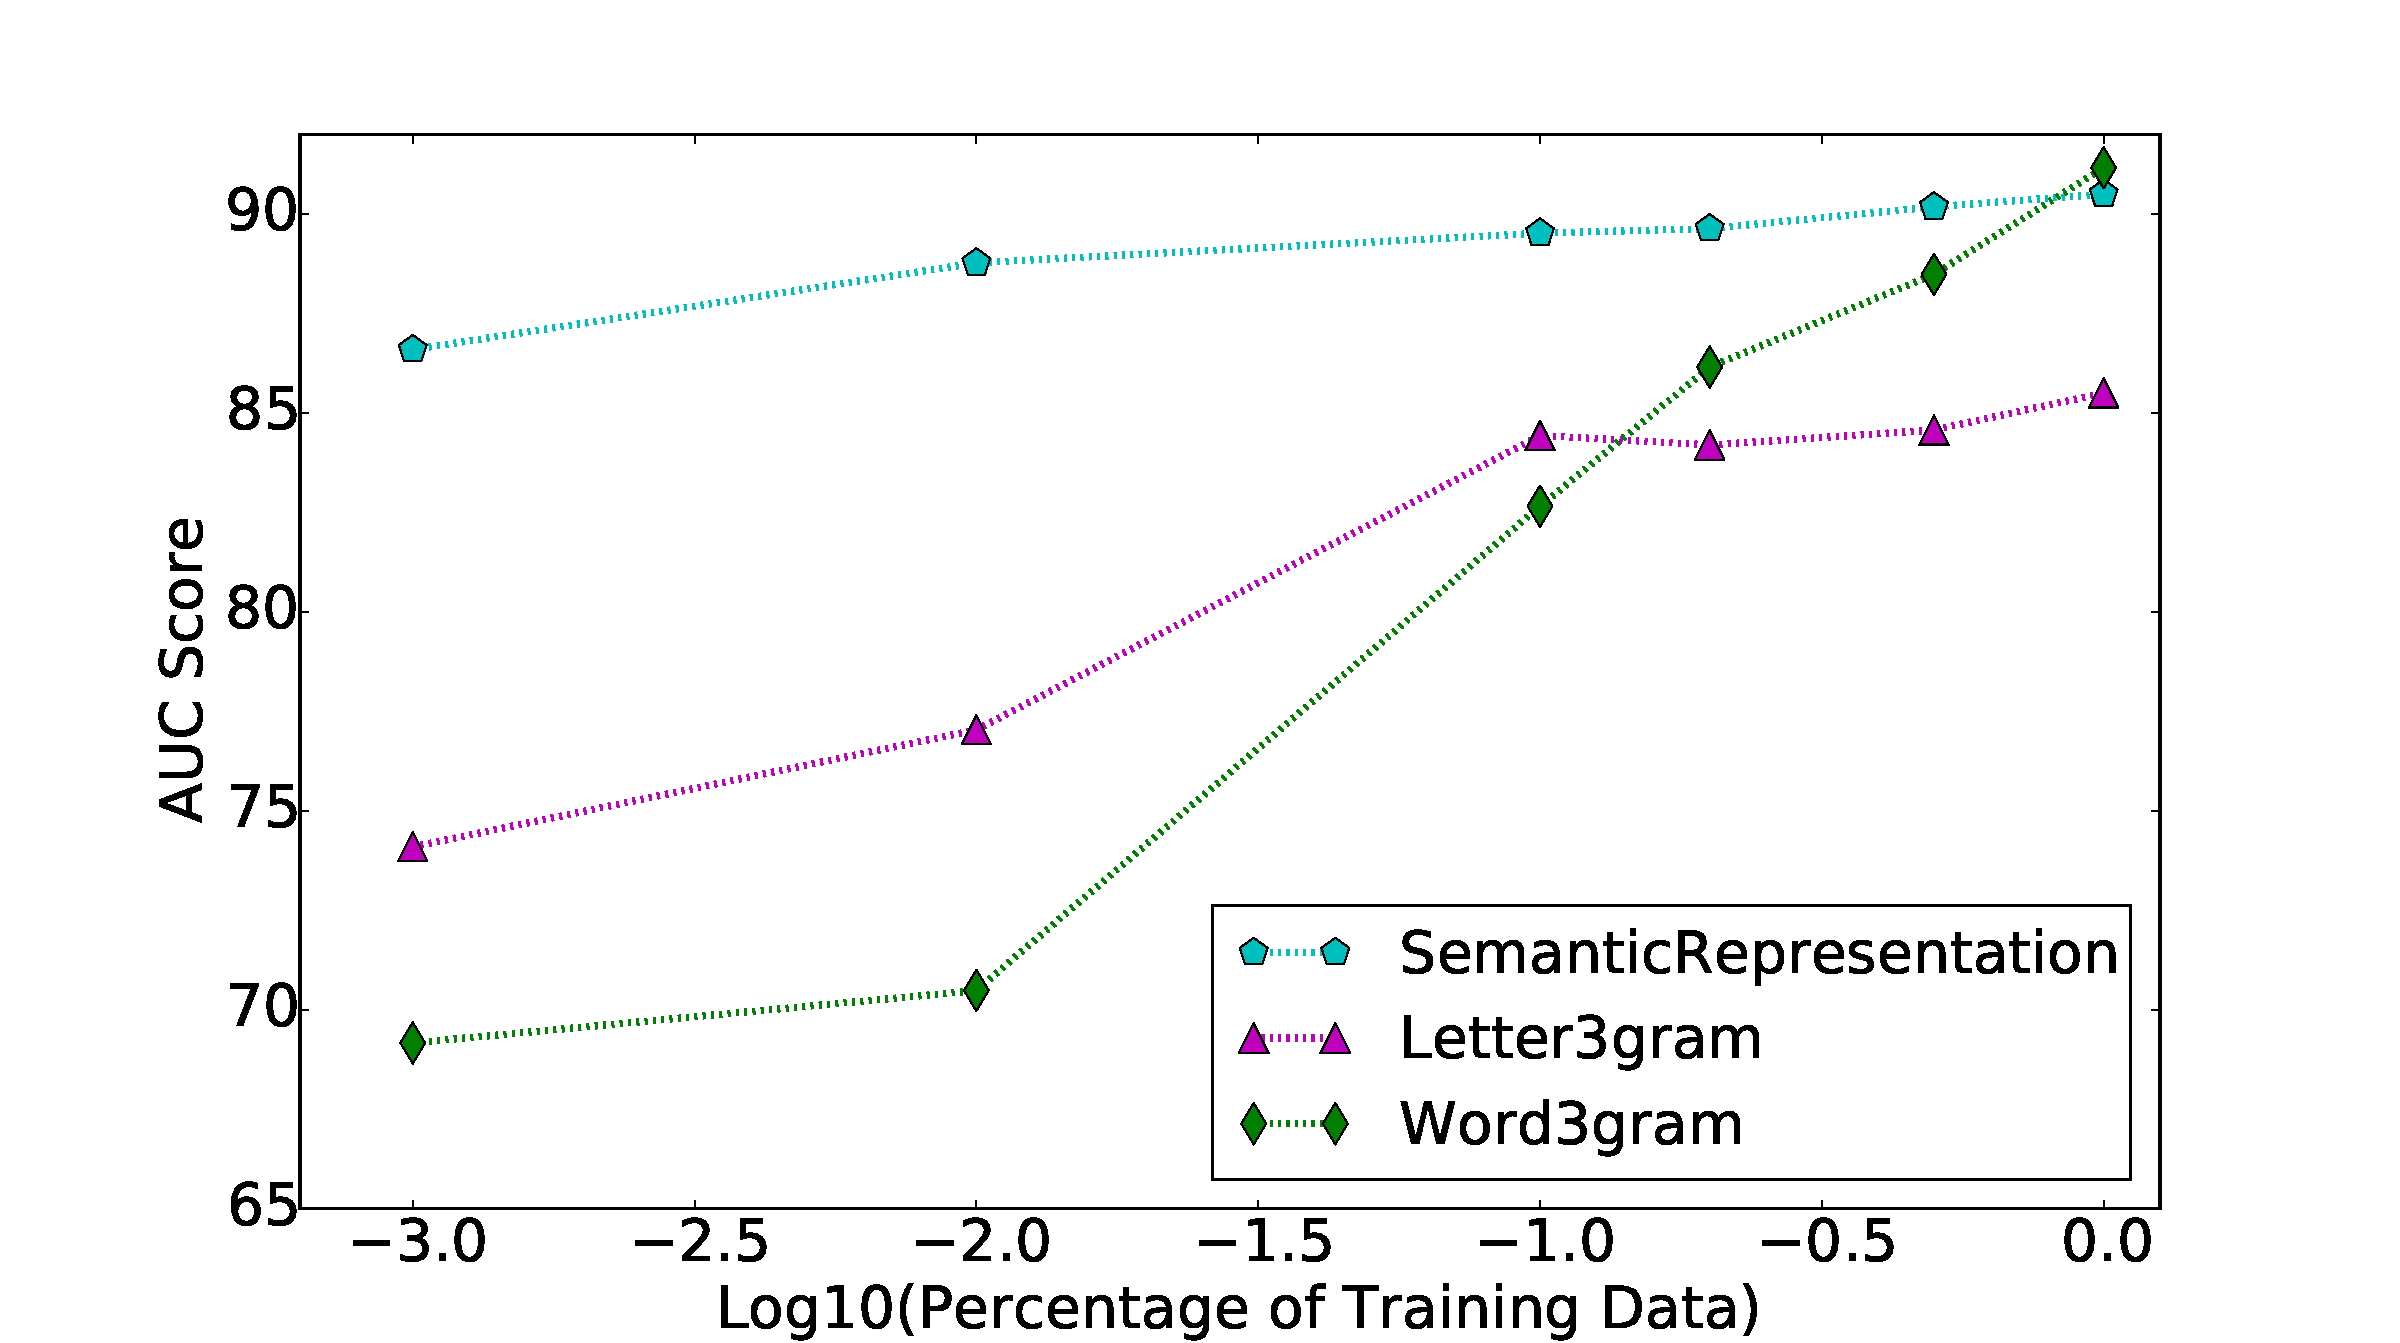
\includegraphics[scale=0.15]{figs/liu15multitask_hotel_svm}
%        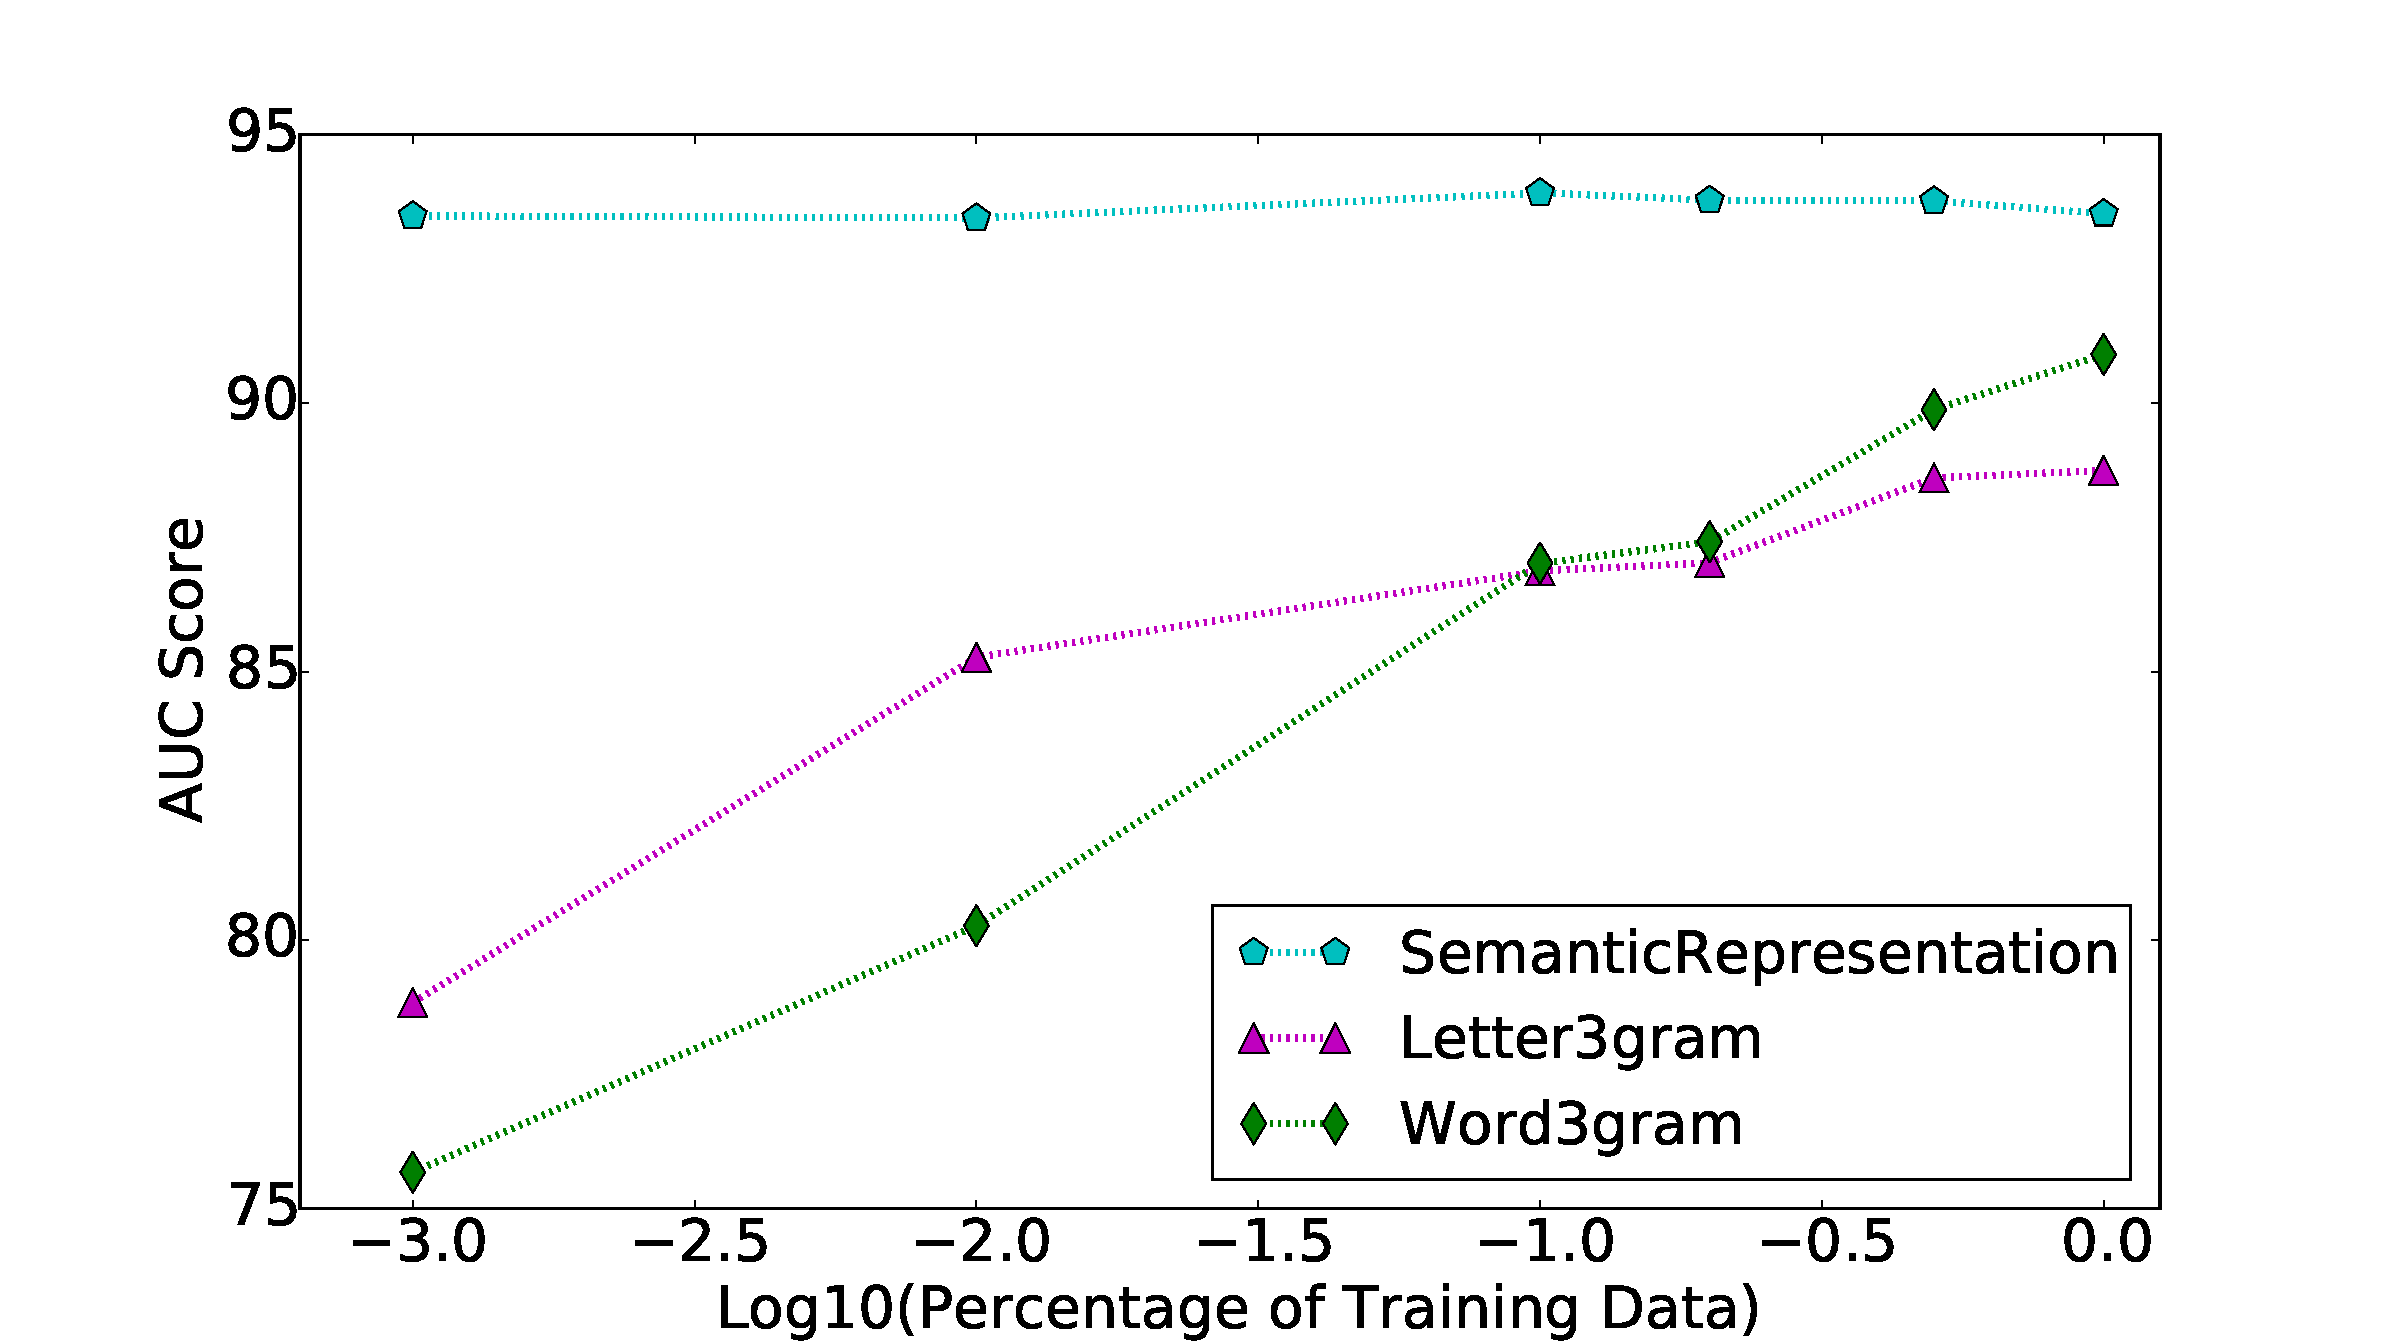
\includegraphics[scale=0.15]{figs/liu15multitask_flight_svm}\\
%        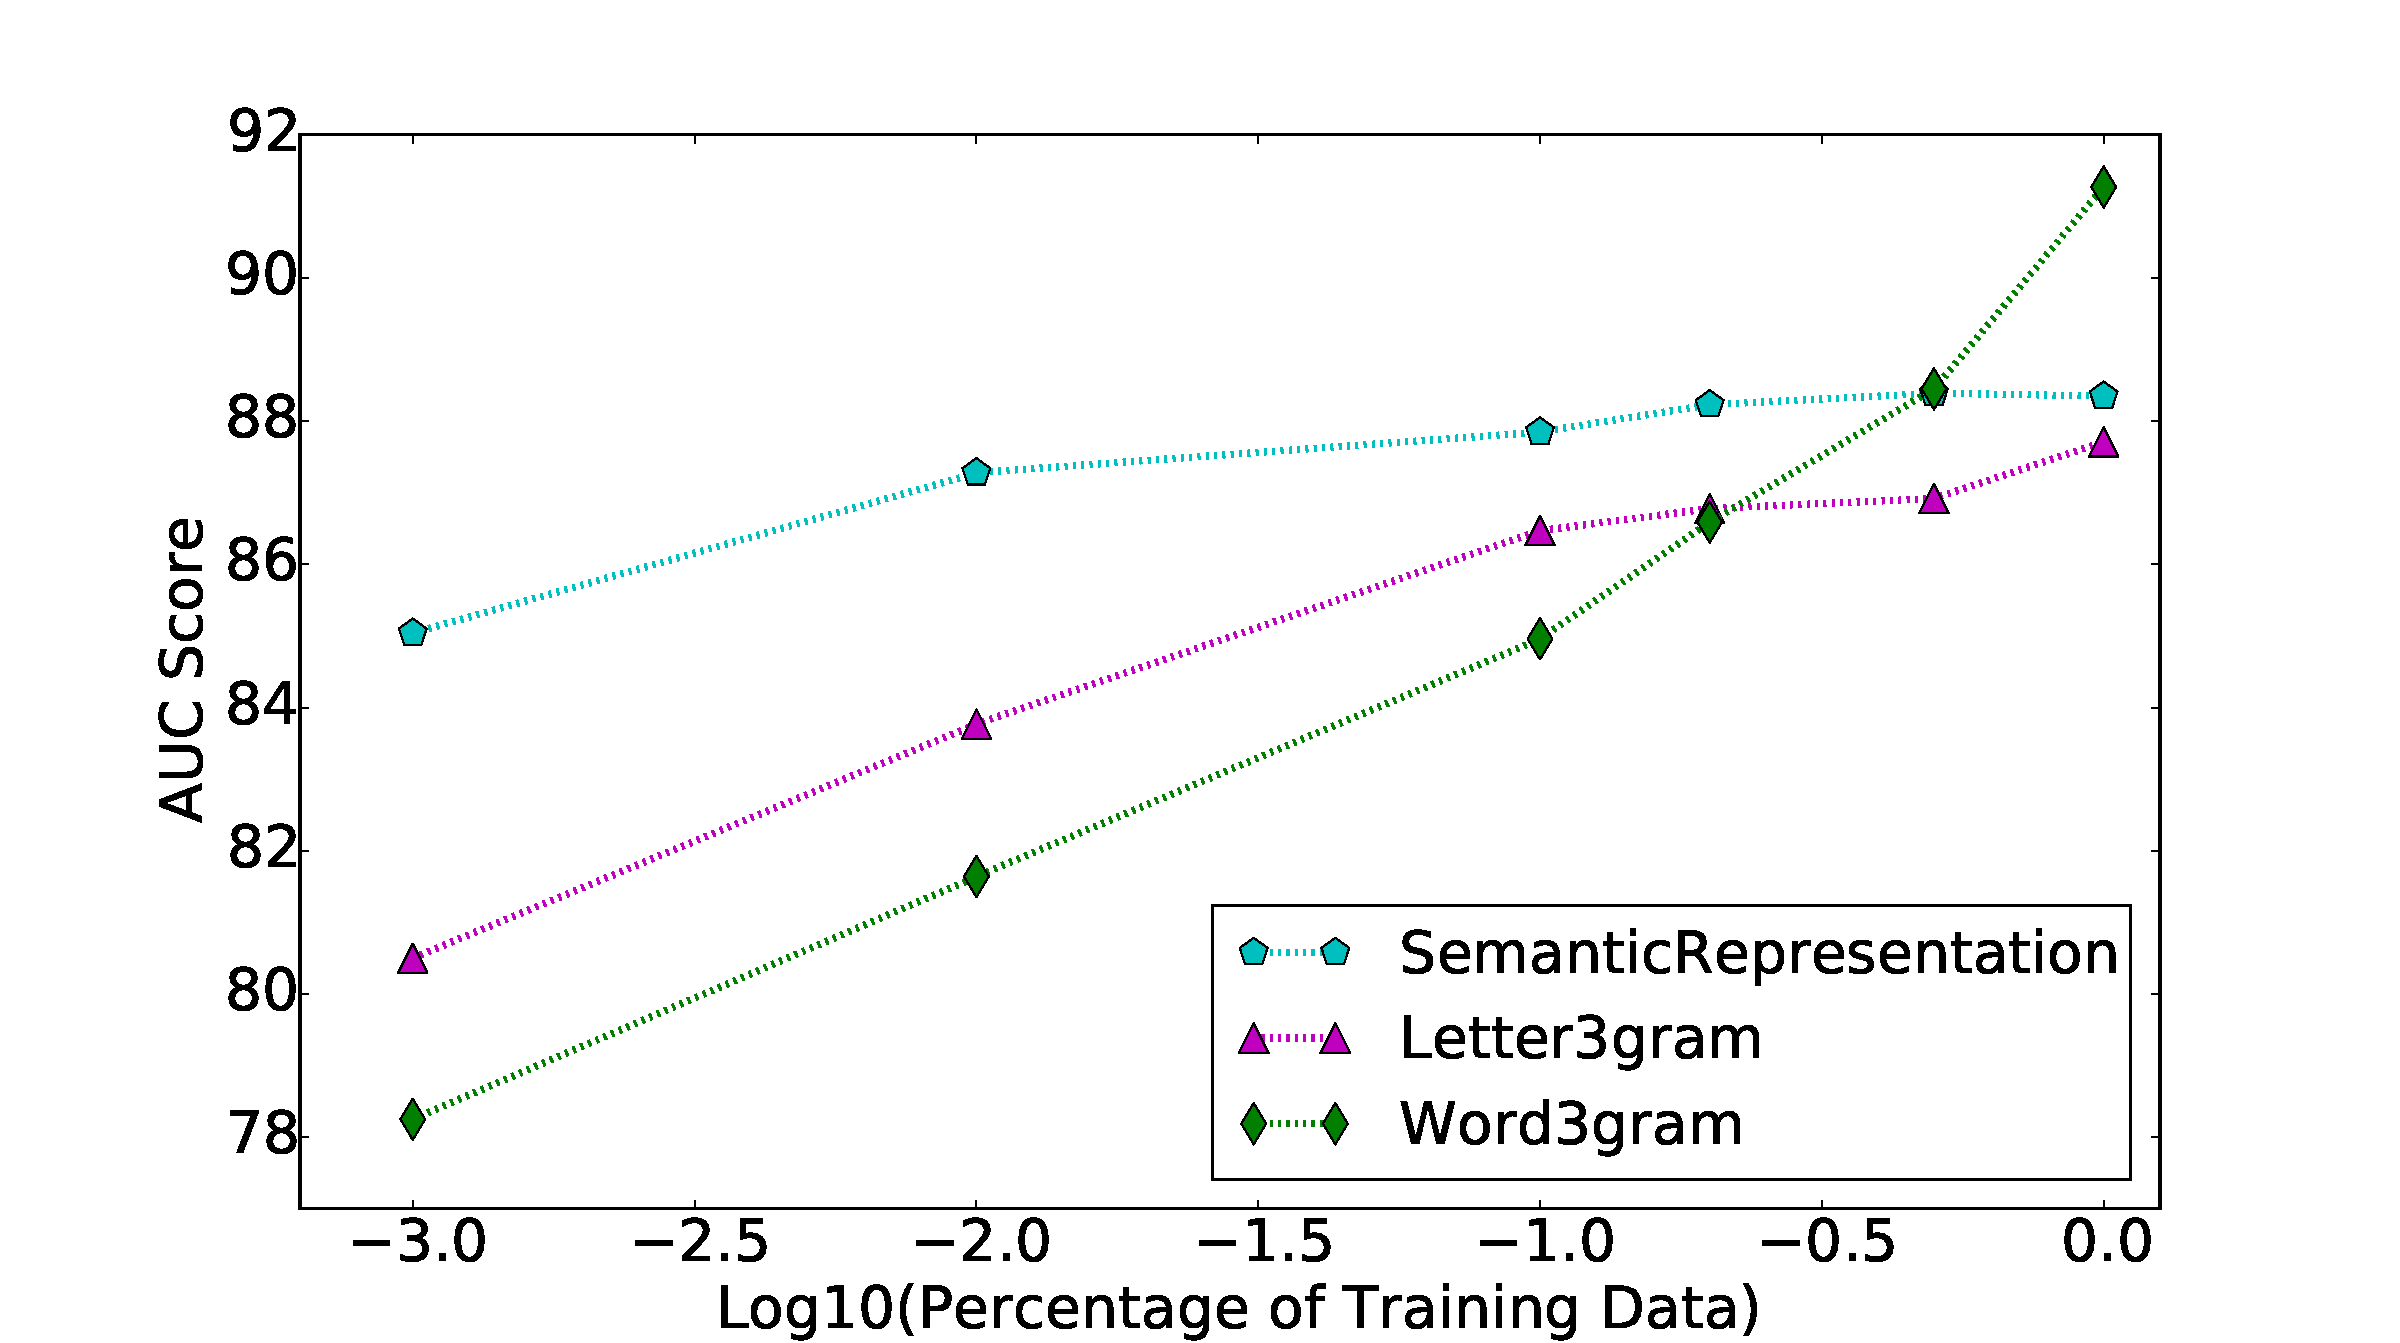
\includegraphics[scale=0.15]{figs/liu15multitask_restaurant_svm}
%        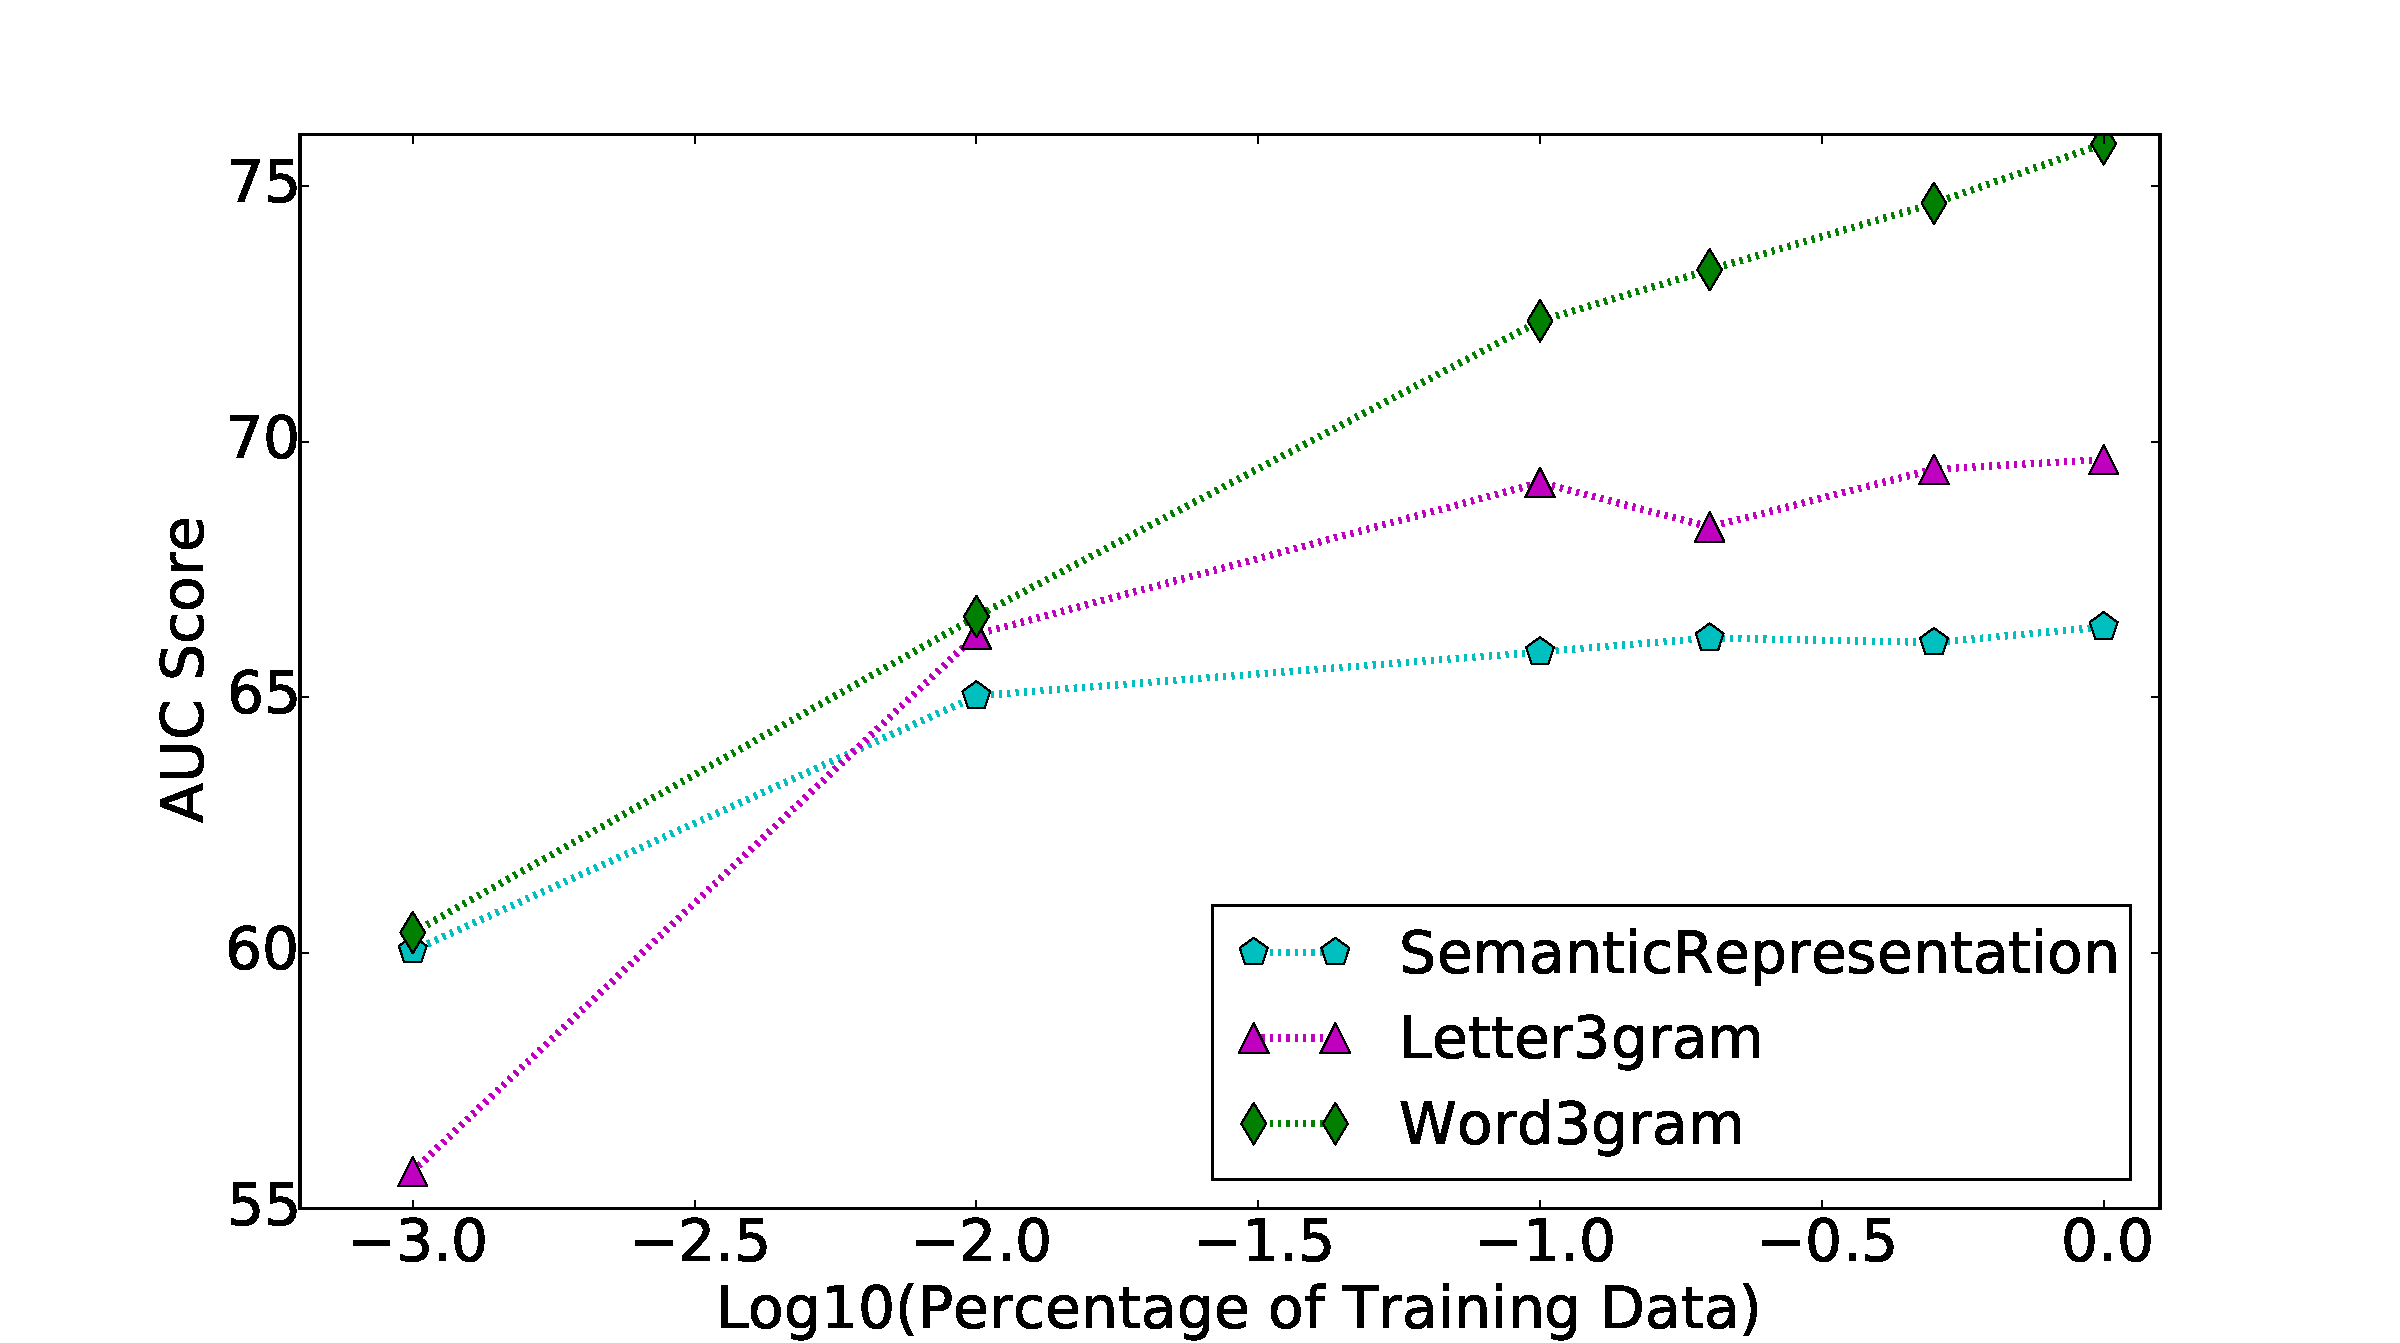
\includegraphics[scale=0.15]{figs/liu15multitask_nightlife_svm}
%
%\end{frame}


%% SUBSECTION%%%%%
\subsection[Infrastructure]{Computational Infrastructure}

%%%%%%
\begin{frame}
\frametitle{A note on Computational Infrastructure}
\bi
\pause
\item We always do our best: use biggest computer and largest dataset
\pause 
\item Don't pre-maturely performance-optimize your code/hardware
	\bi
	\item But be aware of ongoing efforts: \cite{coates13cots,dean12distributed} %TODO newer cites
	\ei
\pause
\item Invest in hyper-parameter tuning
	\bi
	\item Personal preference: I'd choose 10 low-end GeForce GPUs in favor of 1 high-end Tesla GPU to run more tuning experiments in parallel
	\ei
\ei
\end{frame}

\begin{frame}
\frametitle{Lots of hyper-parameters!}
\be
\item Number of layers
\item Number of nodes per layer
\item SGD learning rate
\item Detailed configurations of optimization method
\item Regularization constant
\item Mini-batch size
\item Type of non-linearity
\item Type of distribution for random initialization
\ee
\vspace{1cm}
Important to invest in finding good settings for {\color{red} your data}
\bi
        \item difference between a winning system vs. useless system
\ei
\end{frame}

\begin{frame}
\frametitle{Approaches to hyper-parameter tuning}
\be
\item Exhaustive grid search
\pause
\item Intelligent manual search, a.k.a Graduate Student Descent (GSD)
\pause
\item Treat as a meta machine learning problem \cite{bergstra11hyperparam}
	\bi
        \item Input $x$ = space of hyper-parameters
        \item Output $y$ = validation error after training with given hyper-parameters
        \pause
        \item Computing $y$ is expensive, so we learn a function f(x) that can predict it based on past $(x,y)$ pairs
        		\bi
	        \item e.g. Gaussian Process \cite{bergstra11hyperparam}, Evolutionary Algorithms \cite{moriya15automation}
	        \ei
	\ei
\ee
\pause

Future research: {\color{green} Green Learning}
\bi 
\item energy-efficient \& environmentally-friendly training procedures 
\item someone, please work on this!
\ei
\end{frame}

%%%%%%
\begin{frame}
\frametitle{Section Summary}
\centerline{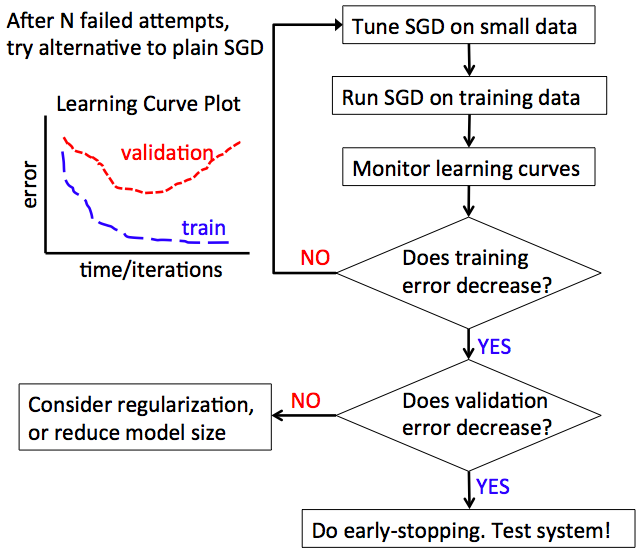
\includegraphics[scale=0.42]{figs/training_recipe}}
\end{frame}




%%% 4. NEW STUFF
%SECTION%%%%%%%%%%%%%%%%%%%
\section[New Stuff]{4. New and Exciting Stuff}
\begin{frame}
\small{\frametitle{Outline}
\tableofcontents
}
\end{frame}
%%%%%%%%%%%%%%%%%%%%


%% SUBSECTION%%%%%
\subsection[Encoder-Decoder]{Encoder-Decoder Architectures}

%%%
\begin{frame}
\frametitle{So far, we've focused on classification}
\bi
\item Many interesting real-world problems are more complex
\item e.g. Structured prediction, Generation
\item Encoder-Decoders*: a general term for architectures that solve the above 
	\bi
	\item Encodes input $\bf{x}$ (e.g. image) into some representation
	\item Decodes representation to generate structured output $\bf{y}$ (e.g. sentence caption)
	\ei
\ei
\blfootnote{*Not to be confused with auto-encoders}
\end{frame}

%%%
\begin{frame}
\frametitle{Encoder-Decoder explanation (1)}
Recall the recurrent neural net (RNN)\\[0.2cm]
Final hidden state $\bf{c}$ can be used as "encoding" of sequence
\centerline{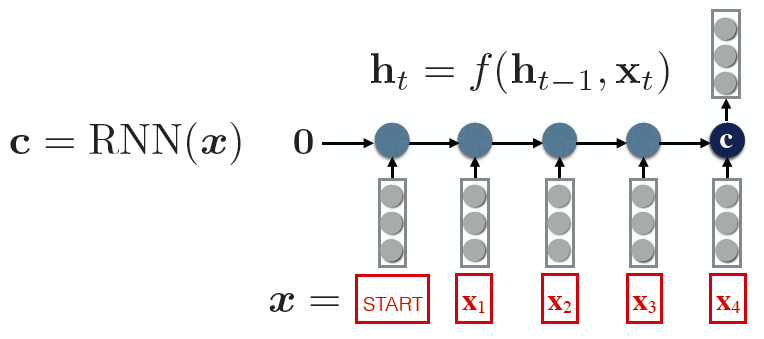
\includegraphics[scale=0.4]{figs/explain_encdec1}}
\end{frame}

%%%
\begin{frame}
\frametitle{Encoder-Decoder explanation (2)}
Recall the recurrent neural net (RNN)\\[0.2cm]
Training objective: predict next word (classification)
\centerline{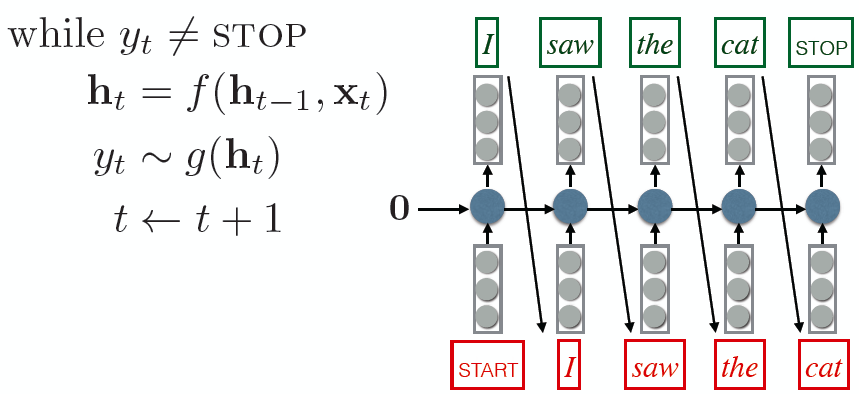
\includegraphics[scale=0.35]{figs/explain_encdec2}}
\end{frame}

%%%
\begin{frame}
\frametitle{Encoder-Decoder explanation (3)}
Simplest Encoder-Decoder: \\[0.2cm]
One RNN for encoding, another RNN for decoding
\bi
\item Decoding can be done by beam search until stop symbol
\item Active research: what is the best encoder or decoder for a specific problem?
\ei
\centerline{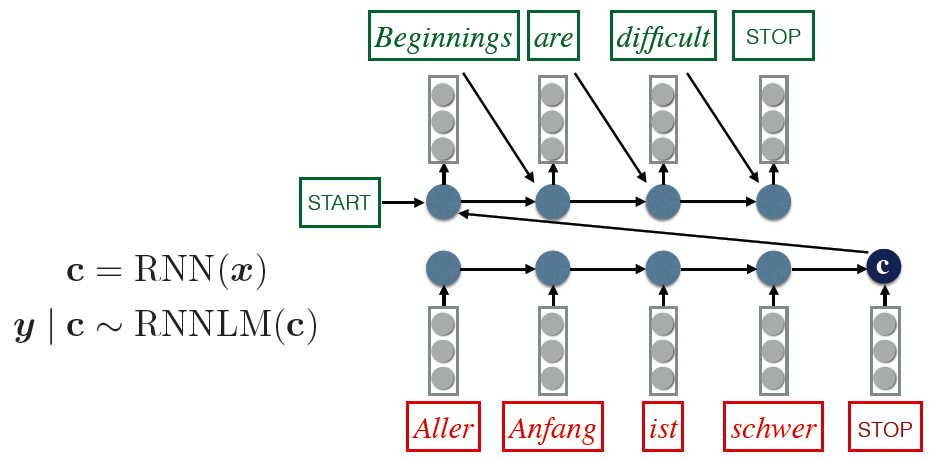
\includegraphics[scale=0.32]{figs/explain_encdec3}}
\end{frame}

%%%
\begin{frame}
\frametitle{Encoder-Decoders for Machine Translation \cite{sutskevar14sequence}}
\begin{scriptsize}("A B C" is source sentence; "W X Y Z" is target sentence)\\Each block is a (deep) LSTM\end{scriptsize}
\centerline{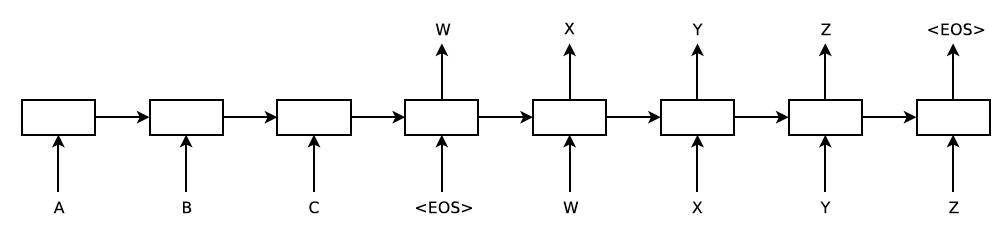
\includegraphics[scale=0.3]{figs/sutskevar14model}}
\bi
\item Training procedure
	\be
	\item Encode source sentence as vector $\bf{c}$
	\item Condition on $\bf{c}$, generate target sentence
	\item Back-prop to optimize target likelihood 
	\ee
\item See \cite{cho14phrase,kalchbrenner13} for other encoder-decoder architecture
\ei
\end{frame}

%%%
\begin{frame}
\frametitle{Encoder-Decoders for Handwriting Generation} 
% TODO: citation, change handwriting example
\centerline{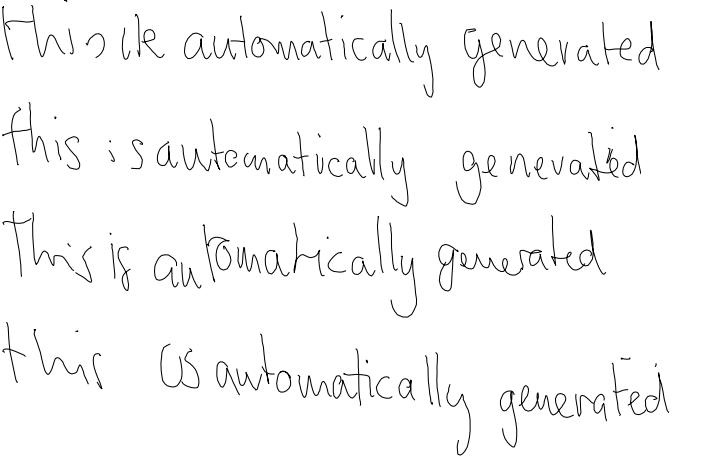
\includegraphics[scale=0.33]{figs/alexgraves_handwriting}}
\url{http://www.cs.toronto.edu/~graves/handwriting.html}
\end{frame}


%% SUBSECTION%%%%%
\subsection[Attention/Memory]{Attention and Memory Mechanism}

%%%
\begin{frame}
\frametitle{Attention: one motivation \cite{bahdanau14translate}}
\bi
\item It seems too much to expect one vector encoding of input $\bf{c}$ can do everything\pause
\item Idea: During decoding, dynamically {\color{red} pay attention} to different parts of the input.
\ei
\pause
\centerline{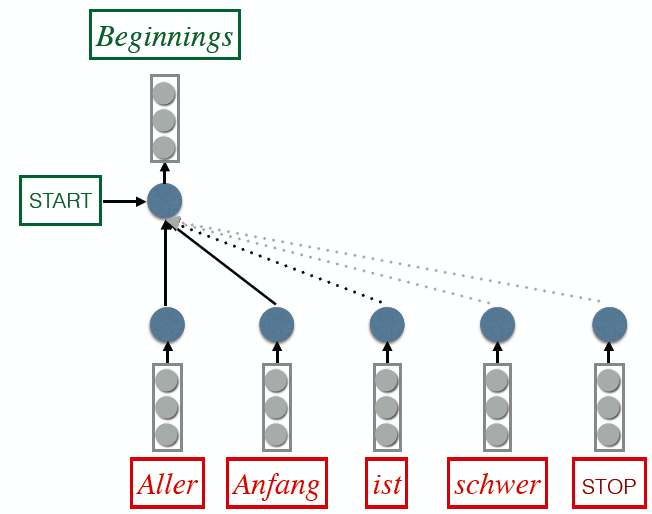
\includegraphics[scale=0.33]{figs/explain_attention1}}
\end{frame}

%%%
\begin{frame}
\frametitle{Attention: one motivation \cite{bahdanau14translate}}
\bi
\item It seems too much to expect one vector encoding of input $\bf{c}$ can do everything
\item Idea: During decoding, dynamically {\color{red} pay attention} to different parts of the input.
\ei
\centerline{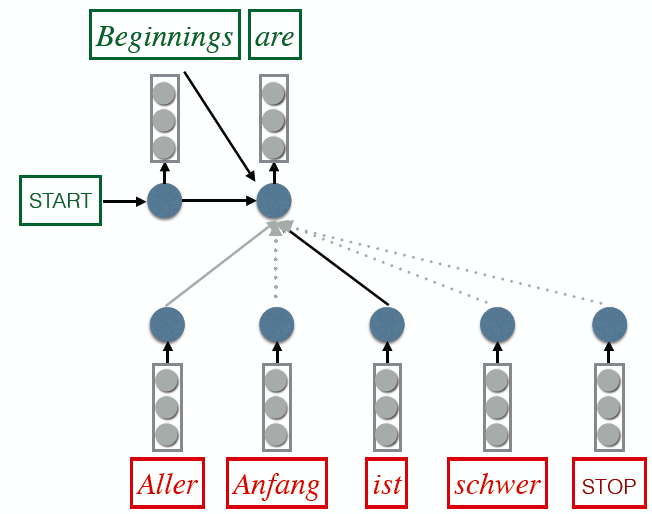
\includegraphics[scale=0.33]{figs/explain_attention2}}
\end{frame}

%%%
\begin{frame}
\frametitle{Attention: one motivation \cite{bahdanau14translate}}
\bi
\item It seems too much to expect one vector encoding of input $\bf{c}$ can do everything
\item Idea: During decoding, dynamically {\color{red} pay attention} to different parts of the input.
\ei
\centerline{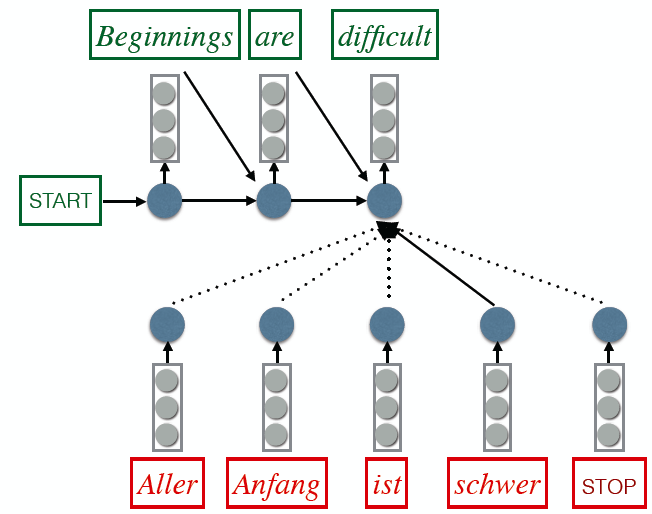
\includegraphics[scale=0.33]{figs/explain_attention3}}
\end{frame}

%%%
\begin{frame}
\frametitle{Attention: one motivation \cite{bahdanau14translate}}
\bi
\item It seems too much to expect one vector encoding of input $\bf{c}$ can do everything
\item Idea: During decoding, dynamically {\color{red} pay attention} to different parts of the input.
\ei
\centerline{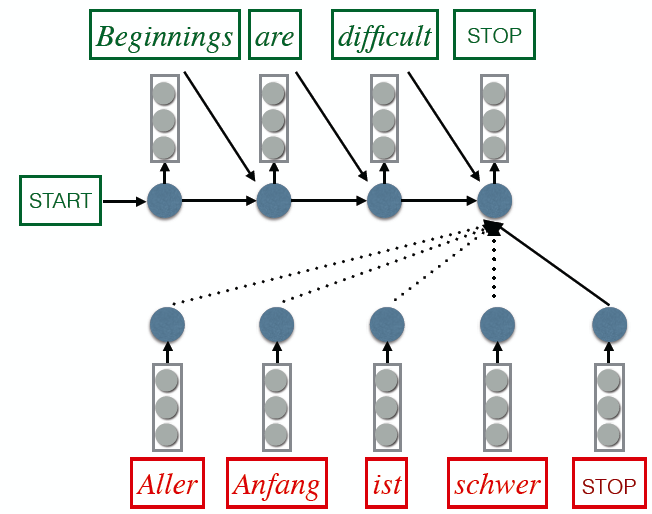
\includegraphics[scale=0.33]{figs/explain_attention4}}
\end{frame}

%%%
\begin{frame}
\frametitle{Encoder-Decoders with Attention}
Caption Generation \cite{xu15caption}: 
\bi
\item Input = image, Output = sentence caption
\item Attention = image patch
\ei
\centerline{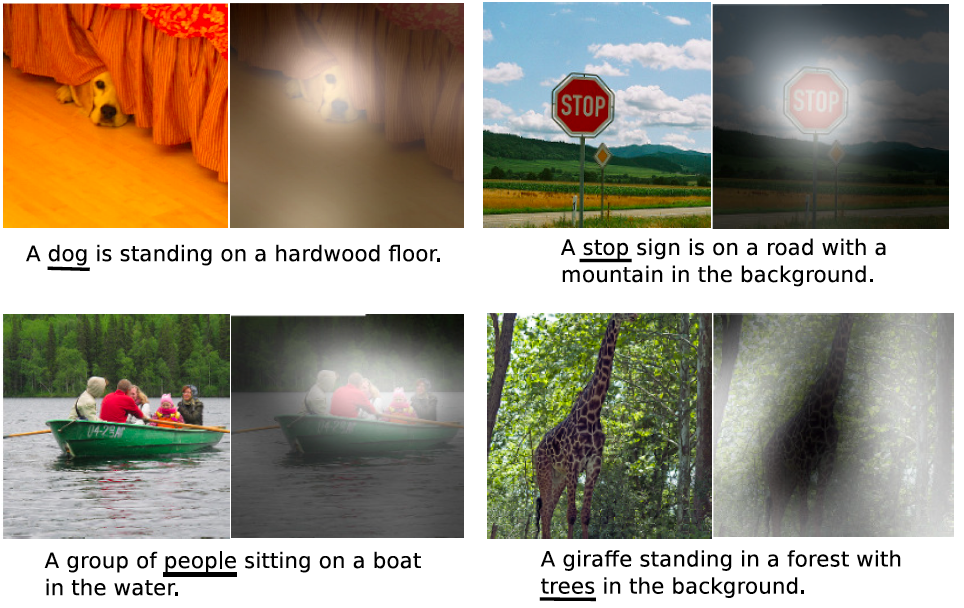
\includegraphics[scale=0.3]{figs/xu15_example}}
\end{frame}

%%%
\begin{frame}
\frametitle{Encoder-Decoders with Attention}
Caption Generation \cite{xu15caption}:
\bi
\item Input = image, Output = sentence caption
\item Attention = image patch
\ei
\centerline{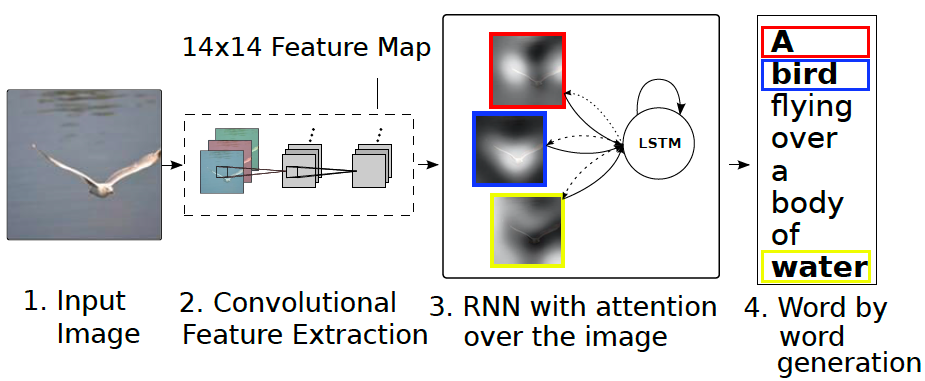
\includegraphics[scale=0.3]{figs/xu15_model}}
\end{frame}

%%%
\begin{frame}
\frametitle{Encoder-Decoders with Attention}
Abstractive Sentence Summarization \cite{rush15abstractive}:
\bi
\item Input = Long sentence, Output = Short sentence
\item Attention = words
\ei
\centerline{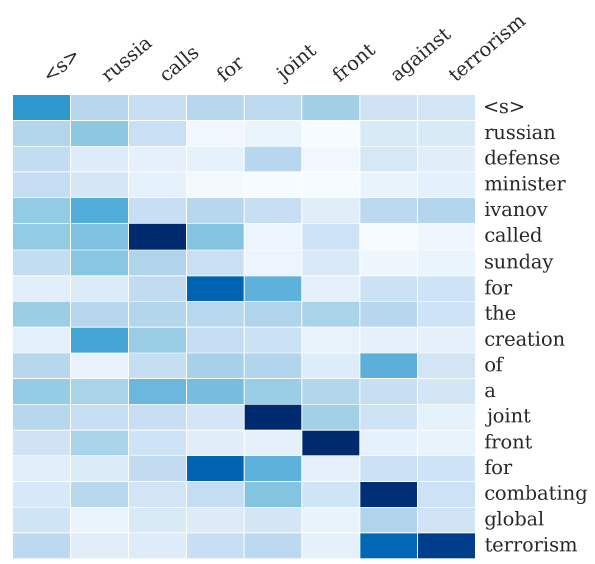
\includegraphics[scale=0.33]{figs/rush15_example}}
\end{frame}

%%%
\begin{frame}
\frametitle{Attention, Memory, and Neural Turing Machines}
\bi
\pause
\item Let's ponder about human learning: \pause
\bi
	\item You can't learn if you don't pay attention \pause
	\item Need to keep relevant concepts in working memory to build up new concepts \pause
\ei
\item Active research: Finding new architectures (preferably differentiable) that allows this kind of learning \cite{graves14turing,weston14memory}
\ei 
\centerline{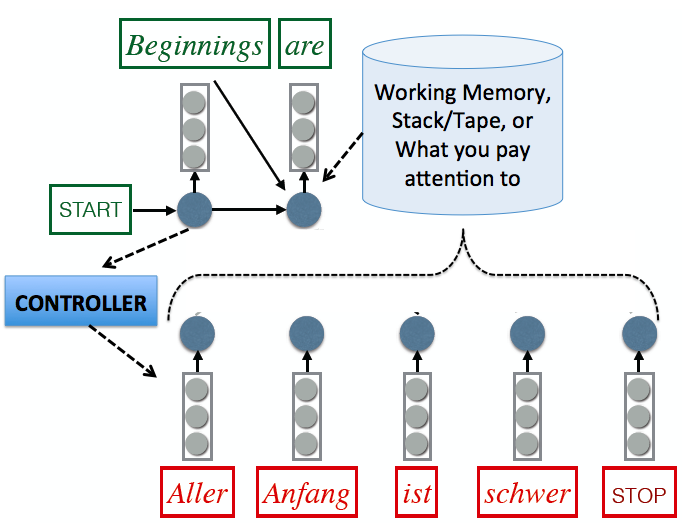
\includegraphics[scale=0.27]{figs/attention_memory_stack}}
\end{frame}


%% SUBSECTION%%%%%
\subsection[Deep Reinforcement]{Deep Reinforcement Learning}

%%%
\begin{frame}
\frametitle{Reinforcement Learning}
\bi
\item Reinforcement Learning can be viewed as general-purpose tool for AI
\bi
	\item We have an {\color{red} agent} with ability to {\color{red} act}
	\item Each {\color{red} action} affects future {\color{red} state}
	\item Plan a set of actions to maximize final {\color{red} reward}
\ei
\pause
\item Policy $\pi$: selects actions given states $a=\pi(s)$
\item Value function $Q^\pi(s,a) = E_\pi[r_{t+1}+\eta r_{t+2} + \eta^2 r_{t+3} \cdots | s,a]$: expected future reward from ($s,a$) under $\pi$ 
\item Optimal Value function $Q^\pi(s,a) = E_\pi[r_{t+1}+\eta r_{t+2} + \eta^2 r_{t+3} \cdots | s,a]$: expected future reward from ($s,a$) under any policy.
\ei
\end{frame}

%%%
\begin{frame}
\frametitle{Deep Reinforcement Learning (Q-learning approach)}
\bi 
\item Estimate value function by neural net: $Q(s,a;w) \approx Q^\pi(s,a)$
\item Training objective: mean square error of Q-values: 
\begin{math}
L(w)=E[\left(y - Q(s,a;w)\right)^2]
\end{math}\\[0.2cm]
where $y= E[r+\eta \max_{a'} Q(s',a'; w_{previous}) | s,a] $ is optimal value under previous weights
\item Train by playing out the actions. See \cite{mnih13atari} for important tricks to get it working
\ei
\end{frame}

%%%
\begin{frame}
\frametitle{Deep Reinforcement Learning for Playing Atari \cite{mnih13atari}}
\centerline{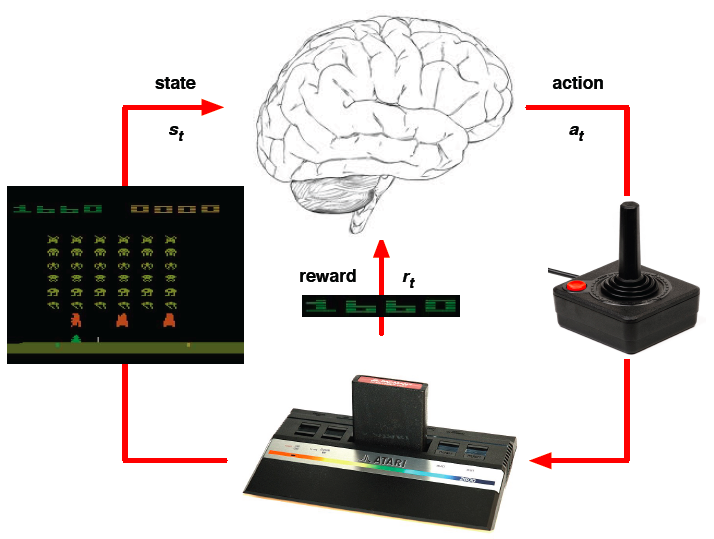
\includegraphics[scale=0.4]{figs/dqn_atari}}
\small{Figure from D. Silver's ICLR2015 keynote slides}
\end{frame}


%% SUBSECTION%%%%%
\subsection[Variational Auto-Encoder]{Auto-Encoding Variational Bayes}

%%%%%%
\begin{frame}
\frametitle{Motivation: Directed Probabilistic Models}
\bi
\item How to perform learning and inference on directed probabilistic models, in the presence of continuous latent variables with intractable posteriors? \pause
\item Generative process:
	\be
	\item Draw continuous latent variable $\bf{z}$ $\sim$ prior $p_{\theta^*}(\bf{z})$ 
	\item Draw data $\bf{x}$ $\sim$ $p_{\theta^*}(\bf{x}|\bf{z})$ 
	\ee 
	\bi
	\item True $\bf{z}$ for each data and parameter $\theta^*$ are unknown
	\ei
	\centerline{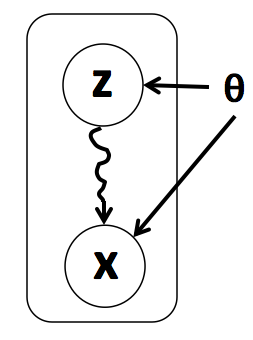
\includegraphics[scale=0.2]{figs/autoencoding_variationalbayes1}}
	\pause
\item Assume marginal likelihood $p_{\theta}(\bf{x})$ and posterior $p_{\theta}(\bf{z}|\bf{x})$ are intractable. Can't differentiate likelihood. Can't do EM.
\ei

\end{frame}

%%%
\begin{frame}
\frametitle{Autoencoding Variational Bayes \cite{kingma14variational}}
\bi
\item Idea: Introduce {\color{red} recognition model} $p_{\phi}(\bf{z}|\bf{x})$ as approximation to posterior $p_{\theta}(\bf{z}|\bf{x})$. 
\item Unlike mean-field variational inference, it's not factorial \& parameters need not be computed in closed-form.\pause
\item Reparameterize ${\bf{\hat{z}}} \sim p_{\phi}(\bf{z}|\bf{x})$ as ${\bf{\hat{z}}} = g_{\phi}(\bf{x}, \epsilon)$
	\bi
	\item $g_\phi()$ is non-linear transform, e.g. MLP
	\item $\epsilon$ is drawn from noise distribution
	\item Using this, one can take derivative of VB bound!\pause
	\ei
\item Implications:
\bi
	\item Training deep generative models on large data
	\item Semi-supervised learning \cite{kingma14ssl}
\ei
\ei
\end{frame}


%%%%%%
\begin{frame}
\frametitle{Section Summary}
\bi
\item Encoder-Decoder Architectures
\item Attention and Memory Mechanism
\item Deep Reinforcement Learning
\item Auto-Encoding Variational Bayes
\ei 
\end{frame}





\begin{frame}
\small{
\frametitle{Review: what we covered}
\tableofcontents
}
\end{frame}

\begin{frame}
\frametitle{Roadmap next}
\be
\item We've covered general background in deep learning
\item {\color{red} Dr. Tsuyoshi Okita}: Deep learning / Neural Nets in NLP
\item {\color{red} Prof. Hermann Ney}: Neural Nets for MT
\item {\color{red} Prof. Kyunghyun Cho}: Neural Nets as MT
\ee
\end{frame}
%%%%%%%%%%%%%%%%%%%%
\begin{frame}[allowframebreaks]
%\frametitle{References}
\begin{tiny}
References:
\bibliographystyle{apalike}
\bibliography{mybib}
\end{tiny}
\end{frame}

\end{document}
